\documentclass{article}

% packages
  % basic stuff for rendering math
  \usepackage[letterpaper, top=1in, bottom=1in, left=1in, right=1in]{geometry}
  \usepackage[utf8]{inputenc}
  \usepackage[english]{babel}
  \usepackage{amsmath} 
  \usepackage{amssymb}
  % \usepackage{amsthm}

  % extra math symbols and utilities
  \usepackage{mathtools}        % for extra stuff like \coloneqq
  \usepackage{mathrsfs}         % for extra stuff like \mathsrc{}
  \usepackage{centernot}        % for the centernot arrow 
  \usepackage{bm}               % for better boldsymbol/mathbf 
  \usepackage{enumitem}         % better control over enumerate, itemize
  \usepackage{hyperref}         % for hypertext linking
  \usepackage{fancyvrb}          % for better verbatim environments
  \usepackage{newverbs}         % for texttt{}
  \usepackage{xcolor}           % for colored text 
  \usepackage{listings}         % to include code
  \usepackage{lstautogobble}    % helper package for code
  \usepackage{parcolumns}       % for side by side columns for two column code
  

  % page layout
  \usepackage{fancyhdr}         % for headers and footers 
  \usepackage{lastpage}         % to include last page number in footer 
  \usepackage{parskip}          % for no indentation and space between paragraphs    
  \usepackage[T1]{fontenc}      % to include \textbackslash
  \usepackage{footnote}
  \usepackage{etoolbox}

  % for custom environments
  \usepackage{tcolorbox}        % for better colored boxes in custom environments
  \tcbuselibrary{breakable}     % to allow tcolorboxes to break across pages

  % figures
  \usepackage{pgfplots}
  \pgfplotsset{compat=1.18}
  \usepackage{float}            % for [H] figure placement
  \usepackage{tikz}
  \usepackage{tikz-cd}
  \usepackage{circuitikz}
  \usetikzlibrary{arrows}
  \usetikzlibrary{positioning}
  \usetikzlibrary{calc}
  \usepackage{graphicx}
  \usepackage{caption} 
  \usepackage{subcaption}
  \captionsetup{font=small}

  % for tabular stuff 
  \usepackage{dcolumn}

  \usepackage[nottoc]{tocbibind}
  \pdfsuppresswarningpagegroup=1
  \hfuzz=5.002pt                % ignore overfull hbox badness warnings below this limit

% New and replaced operators
  \DeclareMathOperator{\Tr}{Tr}
  \DeclareMathOperator{\Sym}{Sym}
  \DeclareMathOperator{\Span}{span}
  \DeclareMathOperator{\im}{Im}
  \DeclareMathOperator{\Div}{div}
  \DeclareMathOperator{\curl}{curl}
  \DeclareMathOperator{\GL}{GL}
  \DeclareMathOperator{\SU}{SU}
  \DeclareMathOperator{\SL}{SL}
  \DeclareMathOperator{\GA}{GA}
  \DeclareMathOperator{\std}{std}
  \DeclareMathOperator{\Cov}{Cov}
  \DeclareMathOperator{\Var}{Var}
  \DeclareMathOperator{\Corr}{Corr}
  \DeclareMathOperator{\Int}{Int}
  \DeclareMathOperator{\Id}{Id}
  \DeclareMathOperator{\Lie}{Lie}
  \DeclareMathOperator{\Hom}{Hom}
  \DeclareMathOperator{\Alt}{Alt}
  \DeclareMathOperator{\rank}{rank}
  \DeclareMathOperator{\conv}{conv}
  \DeclareMathOperator{\aff}{aff}
  \DeclareMathOperator{\arccot}{arccot}
  \DeclareMathOperator*{\argmin}{\arg\!\min}
  \DeclareMathOperator*{\argmax}{\arg\!\max}
  \newcommand{\ket}[1]{\ensuremath{\left|#1\right\rangle}}
  \newcommand{\bra}[1]{\ensuremath{\left\langle#1\right|}}
  \newcommand{\braket}[2]{\langle #1 | #2 \rangle}
  \newcommand{\qed}{\hfill$\blacksquare$}     % I like QED squares to be black

% Custom Environments
  \newtcolorbox[auto counter, number within=section]{question}[1][]
  {
    colframe = orange!25,
    colback  = orange!10,
    coltitle = orange!20!black,  
    breakable, 
    title = \textbf{Question \thetcbcounter ~(#1)}
  }

  \newtcolorbox[auto counter, number within=section]{exercise}[1][]
  {
    colframe = teal!25,
    colback  = teal!10,
    coltitle = teal!20!black,  
    breakable, 
    title = \textbf{Exercise \thetcbcounter ~(#1)}
  }
  \newtcolorbox[auto counter, number within=section]{solution}[1][]
  {
    colframe = violet!25,
    colback  = violet!10,
    coltitle = violet!20!black,  
    breakable, 
    title = \textbf{Solution \thetcbcounter}
  }
  \newtcolorbox[auto counter, number within=section]{lemma}[1][]
  {
    colframe = red!25,
    colback  = red!10,
    coltitle = red!20!black,  
    breakable, 
    title = \textbf{Lemma \thetcbcounter ~(#1)}
  }
  \newtcolorbox[auto counter, number within=section]{theorem}[1][]
  {
    colframe = red!25,
    colback  = red!10,
    coltitle = red!20!black,  
    breakable, 
    title = \textbf{Theorem \thetcbcounter ~(#1)}
  } 
  \newtcolorbox[auto counter, number within=section]{proposition}[1][]
  {
    colframe = red!25,
    colback  = red!10,
    coltitle = red!20!black,  
    breakable, 
    title = \textbf{Proposition \thetcbcounter ~(#1)}
  } 
  \newtcolorbox[auto counter, number within=section]{corollary}[1][]
  {
    colframe = red!25,
    colback  = red!10,
    coltitle = red!20!black,  
    breakable, 
    title = \textbf{Corollary \thetcbcounter ~(#1)}
  } 
  \newtcolorbox[auto counter, number within=section]{proof}[1][]
  {
    colframe = orange!25,
    colback  = orange!10,
    coltitle = orange!20!black,  
    breakable, 
    title = \textbf{Proof. }
  } 
  \newtcolorbox[auto counter, number within=section]{definition}[1][]
  {
    colframe = yellow!25,
    colback  = yellow!10,
    coltitle = yellow!20!black,  
    breakable, 
    title = \textbf{Definition \thetcbcounter ~(#1)}
  } 
  \newtcolorbox[auto counter, number within=section]{example}[1][]
  {
    colframe = blue!25,
    colback  = blue!10,
    coltitle = blue!20!black,  
    breakable, 
    title = \textbf{Example \thetcbcounter ~(#1)}
  } 
  \newtcolorbox[auto counter, number within=section]{code}[1][]
  {
    colframe = green!25,
    colback  = green!10,
    coltitle = green!20!black,  
    breakable, 
    title = \textbf{Code \thetcbcounter ~(#1)}
  } 

  \BeforeBeginEnvironment{example}{\savenotes}
  \AfterEndEnvironment{example}{\spewnotes}
  \BeforeBeginEnvironment{lemma}{\savenotes}
  \AfterEndEnvironment{lemma}{\spewnotes}
  \BeforeBeginEnvironment{theorem}{\savenotes}
  \AfterEndEnvironment{theorem}{\spewnotes}
  \BeforeBeginEnvironment{corollary}{\savenotes}
  \AfterEndEnvironment{corollary}{\spewnotes}
  \BeforeBeginEnvironment{proposition}{\savenotes}
  \AfterEndEnvironment{proposition}{\spewnotes}
  \BeforeBeginEnvironment{definition}{\savenotes}
  \AfterEndEnvironment{definition}{\spewnotes}
  \BeforeBeginEnvironment{exercise}{\savenotes}
  \AfterEndEnvironment{exercise}{\spewnotes}
  \BeforeBeginEnvironment{proof}{\savenotes}
  \AfterEndEnvironment{proof}{\spewnotes}
  \BeforeBeginEnvironment{solution}{\savenotes}
  \AfterEndEnvironment{solution}{\spewnotes}
  \BeforeBeginEnvironment{question}{\savenotes}
  \AfterEndEnvironment{question}{\spewnotes}
  \BeforeBeginEnvironment{code}{\savenotes}
  \AfterEndEnvironment{code}{\spewnotes}

  \definecolor{dkgreen}{rgb}{0,0.6,0}
  \definecolor{gray}{rgb}{0.5,0.5,0.5}
  \definecolor{mauve}{rgb}{0.58,0,0.82}
  \definecolor{lightgray}{gray}{0.93}

  % default options for listings (for code)
  \lstset{
    autogobble,
    frame=ltbr,
    language=C,                           % the language of the code
    aboveskip=3mm,
    belowskip=3mm,
    showstringspaces=false,
    columns=fullflexible,
    keepspaces=true,
    basicstyle={\small\ttfamily},
    numbers=left,
    firstnumber=1,                        % start line number at 1
    numberstyle=\tiny\color{gray},
    keywordstyle=\color{blue},
    commentstyle=\color{dkgreen},
    stringstyle=\color{mauve},
    backgroundcolor=\color{lightgray}, 
    breaklines=true,                      % break lines
    breakatwhitespace=true,
    tabsize=3, 
    xleftmargin=2em, 
    framexleftmargin=1.5em, 
    stepnumber=1
  }

% Page style
  \pagestyle{fancy}
  \fancyhead[L]{Abstract Algebra}
  \fancyhead[C]{Muchang Bahng}
  \fancyhead[R]{August 2021} 
  \fancyfoot[C]{\thepage / \pageref{LastPage}}
  \renewcommand{\footrulewidth}{0.4pt}          % the footer line should be 0.4pt wide
  \renewcommand{\thispagestyle}[1]{}  % needed to include headers in title page

\begin{document}

\title{Abstract Algebra}
\author{Muchang Bahng}
\date{Spring 2024}

\maketitle
\tableofcontents
\pagebreak

\section{Algebraic Structures}

    \begin{definition}
      An \textit{operation} $*$ on a set $M$ is a map 
      \begin{equation}
         \ast : M \times M \longrightarrow M
      \end{equation}
    \end{definition}

    \begin{example}
      Regular addition $+$ and multiplication $\times$ are operations in $\mathbb{R}$, $\mathbb{Q}$, and $\mathbb{N}$, but multiplication is not defined in $\mathbb{R_{-}}$, since the product of 2 negative numbers is a positive number. 
      \end{example}

    \begin{example}
      The product of functions $f: N \longrightarrow M$ and $g: P \longrightarrow N$ is defined as the composition of them
      \begin{equation}
        (f \circ g)(x) \equiv f(g(x)) \; \forall x\in P
      \end{equation}
    \end{example}

    \begin{example}
      $\mathbb{R}^{3}$ can have operations of vector addition and the cross product. The inner product is \textit{not} an operation on $\mathbb{R}^3$.
    \end{example}

    \begin{definition}
      Let $(M, \circ)$ and $(N, *)$ be two sets with their respective operations. The mapping $f: (M, \circ) \longrightarrow (N, *)$ is a \textit{homomorphism} if
      \begin{equation}
        f(a \circ b) = f(a) * f(b) \; \forall a, b \in M
      \end{equation}
      A homomorphism is an \textit{isomorphism} if and only if it is bijective. If an isomorphism $f$ exists between two algebraic structures $M$ and $N$, then $M$ and $N$ are said to be \textit{isomorphic}, denoted $M \simeq N$. An homomorphism from structure $G$ to itself is called an \textit{endomorphism}, and an endomorphism that is also an isomorphism is called an automorphism. 
    \end{definition}

    \begin{example}
      The map $a \mapsto 2^{a}$ is an isomorphism between $(\mathbb{R}, +)$ and $(\mathbb{R}^{+}, \times)$ since 
      \begin{equation}
        2^{a+b} = 2^a \times 2^b
      \end{equation}
    \end{example}

    We now define a crucial type of measure on a set, called a relation.  

    \begin{definition}
      given a set $M$, any subset $R \subset M \times M$ is called a \textit{relation} on the set $M$. If $(a, b) \in R$, then $a$ and $b$ are \textit{related}, denoted $a R b$. 
    \end{definition}

    \begin{definition}
      An \textit{equivalence relation} $R$, also written $\sim$, is a relation which is:
      \begin{enumerate}
        \item Reflexive. $a R a$ 
        \item Symmetric. $a R b \iff b R a$ 
        \item Transitive. $a R b, b R c \implies a R c$ 
      \end{enumerate}
      An equivalence relation $R$ defines an \textit{equivalence class} $R(a)$, defined 
      \begin{equation}
        R(a) \equiv \{ b \in M | a\sim b \} 
      \end{equation}
      which directly implies that the set of equivalence classes $\{R(a)\}$ form a partition of $M$. 
    \end{definition}

    \begin{definition}
      The set of equivalence classes under relation $R$ is called the \textit{quotient set} of $M$ by $R$, denoted $\frac{M}{R}$. The map 
      \begin{equation}
        q: M \longrightarrow \frac{M}{R}, \; a \mapsto R(a)
      \end{equation}
      is called the \textit{quotient map}. We can also define an operation $*$ on the quotient set $\frac{M}{R}$ to get $\big( \frac{M}{R}, * \big)$, defined as
      \begin{equation}
        \{a \} * \{ b \} \equiv \{ a * b \}
      \end{equation}
      to turn this quotient set into an algebraic structure. In words, $*$ applied on two classes takes arbitrary representatives of each class, does the operation on each of them, and finally outputs the class of the resulting product. 
    \end{definition}

    \begin{example}
      $M$ is the set of circles in $\mathbb{R}^{2}$. Given $a, b \in M$, $a \sim b$ iff the radii are equal in length. We can denote each equivalence class by $\{ r \}$, where $r$ is the length of the radius. We can define addition as 
      \begin{equation}
        \{ a \} + \{ b \} \equiv \{ a + b\}
      \end{equation}
    \end{example}

  \subsection{Group-like Structures}

    \begin{definition}
      A \textit{groupoid}, also called a \textit{magma}, is a set with operation $(M, *)$ where the operation $*$ is closed. No other properties are imposed. 
    \end{definition}

    \begin{definition}
      A \textit{semigroup} $(M, *)$ is a groupoid where the binary operation $*$ must be associative.  
    \end{definition}

    \begin{definition}
      A \textit{monoid} $(M, *)$ is a semigroup with an identity element $I \in M$ such that given a $m \in M$
      \begin{equation}
        I * m = m * I = m
      \end{equation}
    \end{definition}

    \begin{definition}
      A \textit{group} is a monoid where every element has an inverse element. That is, $(G, *)$ is a set with binary operation having the properties of closure, associativity, existence of an identity and existence of inverses, in the following order: 
      \begin{enumerate}
        \item $x, y \in S \implies x*y, \;y*x \in G$ but not necessarily $x*y  = y*x$
        \item $a*(b*c) = (a*b)*c \; \forall a, b, c \in G$
        \item $\exists I \in G : x*I = I*x = x \; \forall x \in G $
        \item $\forall x \in G \; \exists x^{-1} \in G : x * x^{-1} = x^{-1} * x = I$
      \end{enumerate}
    \end{definition}

    \begin{proposition}
      The identity and the inverse is unique, and for any $a, b$, the equation $x*a = b$ has the unique solution $x = b* a^{-1}$.
    \end{proposition}
    \begin{proof}
       Assume that there are two identities of group $(G,*)$, denoted $I_{1}, I_{2}$, where $I_{1} \neq I_{2}$. According to the properties of identities, $I_{1} = I_{1} * I_{2} = I_{2} \implies I_{1} = I_{2}$. \\
      As for uniqueness of a inverses, let $a$ be an element of $G$, with its inverses $a_{1}^{-1}, a_{2}^{-1}$. Then, 
      \begin{align*}
        a * a_{1}^{-1} = I & \implies a_{2}^{-1} * \Big(a * a_{1}^{-1} \Big)= a_{2}^{-1} * I \\
         & \implies \Big(a_{2}^{-1} * a \Big) * a_{1}^{-1} = a_{2}^{-1} \\
         & \implies I * a_{1}^{-1} = a_{2}^{-1}
      \end{align*}
      Since the inverse is unique, we can operate on each side of the equation $x*a = b$ to get $x*a*a^{-1} = b*a^{1} \implies x * I = x = b*a^{-1}$. Clearly, the derivation of this solution is unique since the elements that we have operated on are unique.
    \end{proof}

    \begin{definition}
      An \textit{abelian group} $(A, +)$ is a group where $+$ is commutative. That is, 
      \begin{equation}
        x+y = y+x \; \forall x, y \in A
      \end{equation}
      The abstract operation for an abelian group is usually called addition. 
    \end{definition}

    \begin{example}
      $\mathbb{Z}, \mathbb{Q}, \mathbb{R}$ are all abelian groups with respect to addition. $\mathbb{Q}^{*} \equiv \mathbb{Q} \setminus \{0\}$ and $\mathbb{R}^{*} \equiv \mathbb{R} \setminus \{0\}$ are abelian groups with respect to multiplication.
    \end{example}

    \begin{example}
      The set of all functions on a given interval $F[a,b]$ is abelian with respect to addition, defined as $(f+g)(x) \equiv f(x) + g(x)$. 
    \end{example}

  \subsection{Ring-like Structures}

    \begin{definition}
      A \textit{ring} is a set $(R, +, \times)$ equipped with two operations, called addition and multiplication. It has properties: 
      \begin{enumerate}
        \item $R$ is an abelian group with respect to $+$.
        \item Multiplication $\times$ is distributive with respect to addition $+$
          \begin{equation}
            a \times (b + c) = a\times b + a\times c, (a+b)\times c = a\times c + b\times c \; \forall a, b, c \in R
          \end{equation}
        \item There is an absorbing element, denoted $0$ such that 
          \begin{equation}
            0\times a = a\times 0 = 0 \; \forall a \in R
          \end{equation}
        \item Equivalence of Additive Inverses
          \begin{equation}
            a \times (-b) = (-a) \times b = - (a\times b)
          \end{equation}
      \end{enumerate}
    \end{definition}

    \begin{definition}
      A ring $R$ is a \textit{commutative ring} if and only if multiplication is commutative, i.e. $a\times b = b \times a \; \forall a, b \in R$. It is an \textit{associative ring} if and only if multiplication is associative, i.e. $a \times (b \times c) = (a \times b) \times c \; \forall a, b, c \in R$.
    \end{definition}

    \begin{definition}
      The \textit{unity} of a ring $R$ is the multiplicative identity, denoted as $1$. 
      \begin{equation}
        a \times 1 = 1 \times a = a \; \forall a \in R
      \end{equation}
      Note that a ring cannot have more than 1 unity, but it may not exist at all. But usually, a ring has a unity.
    \end{definition}

    This is not to be confused with the unit of a ring. 

    \begin{definition}
      A \textit{unit} of a ring $R$ is an element $u \in R$ that has a multiplicative inverse in $R$. 
    \end{definition}

    \begin{example}
      $\mathbb{Z}, \mathbb{Q}, \mathbb{R}$ are commutative, associative rings with respect to ordinary addition and multiplication.
    \end{example}

    \begin{example}
      The set of even integers $2\mathbb{Z}$ is a commutative, associative ring without unity.
    \end{example}

    \begin{proposition}
      Given a set $X$, let $2^X$ be its power set, that is the set of all subsets of $X$. Then, $2^X$ is a commutative associative ring with respect to the operations of symmetric difference (i.e. the set of elements which is in exactly one of the sets) 
      \begin{equation}
        M \bigtriangleup N \equiv (M \setminus N) \cup (N \setminus M)
      \end{equation}
      and intersection $\cap$, taken for addition an multiplication, respectively. 
    \end{proposition}
    \begin{proof}
      We will not prove all of the axioms of the ring, but we can state some important facts about this structure. The additive identity is $\emptyset$ and the multiplicative identity is $X$. Finally, it is clear that 
      \begin{align*}
        & M \bigtriangleup N \equiv (M \setminus N) \cup (N \setminus M) \equiv N \bigtriangleup M \\
        & M \cap N = N \cap M \\
        & M \cap N \cap P = (M \cap N) \cap P = M \cap (N \cap P)
      \end{align*}
    \end{proof}

    \begin{example}
      A \textit{division ring}, also called a \textit{skew field}, is an associative ring with unity where every nonzero element is invertible with respect to $\times$. Division rings differ from fields in that multiplication is not required to be commutative. 
    \end{example}

    At first, a division ring may not seem different from a field. However, a classic example is the ring of invertible matrices, which is not necessarily commutative, but is a ring in which "division" can be done by right and left multiplication of a matrix inverse. 
    \begin{equation}
      a a^{-1} = a^{-1} a = I
    \end{equation}
    This implies that every element in the division ring commutes with the identity, but again commutativity does not necessarily hold for arbitrary elements $a, b$. 

    \begin{definition}
      A \textit{field} $(F, +, \times)$ is a commutative, associative ring with unity where every nonzero element is invertible (with respect to $\times$). It is usually denoted as $\mathbb{F}$. Note that $F$ is now an abelian group with respect to $\times$. 
    \end{definition}

    \begin{definition}
      An element a of a ring $R$ is called a \textit{left zero divisor} if there exists a nonzero $x$ such that $a x = 0$ and a \textit{right zero divisor} if there exists a nonzero $x$ such that $x a = 0$. 
    \end{definition}

    \begin{definition}
      A ring $R$ with no zero divisors for every element is called a \textit{domain}. 
    \end{definition}

    \begin{proposition}
      Every field is a domain. 
    \end{proposition}
    \begin{proof}
      Given $x, y \in \mathbb{F}$, assume $x y = 0$ with $x \neq 0$. Since $x$ is invertible,
      \begin{equation}
        0 = x^{-1} 0 = x^{-1} (x y) = y
      \end{equation}
      Now assuming that $y \neq 0$, since $y$ is invertible, 
      \begin{equation}
        0 = 0 y^{-1} = (x y) y^{-1} = x
      \end{equation}
    \end{proof}

    While the converse is not true, we can state the following result. 

    \begin{theorem}[Wedderburn's little theorem]
      Every finite domain is a field. 
    \end{theorem}

  \subsection{Vector Space Structures}

    \begin{definition}[Vector Space]
       A \textit{vector space over a field $F$} consists of an abelian group $(V, +)$ and an operation called \textit{scalar multiplication} 
       \begin{equation}
         \cdot: F \times V \rightarrow V
       \end{equation}
      such that for all $x, y\in V$ and $\lambda, \mu \in F$, we have 
      \begin{enumerate}
        \item $\lambda \cdot (x + y) = \lambda \cdot x + \lambda \cdot y$
        \item $(\lambda + \mu) \cdot x = \lambda \cdot x + \mu \cdot x$ 
        \item $(\lambda \mu) \cdot x = \lambda \cdot (\mu \cdot x )$, which equals $(\mu \lambda) \cdot x = \mu \cdot (\lambda \cdot x)$ since $F$ is commutative 
        \item $1 \cdot x = x$ , where $1$ is the unity of $F$
      \end{enumerate}
    \end{definition}

    \begin{definition}
      A \textit{left R-module} $M$ consists of an abelian group $(M, +)$ and an operation called \textit{scalar multiplication}
      \begin{equation}
        \cdot: R \times M \longrightarrow M
      \end{equation}
      such that for all $\lambda, \mu \in R$ and $x, y \in M$, we have 
      \begin{enumerate}
        \item $\lambda \cdot (x + y) = \lambda \cdot x + \lambda \cdot y$
        \item $(\lambda + \mu) \cdot x = \lambda \cdot x + \mu \cdot x$ 
        \item $(\lambda \mu) \cdot x = \lambda \cdot (\mu \cdot x )$, not necessarily equaling $(\mu \lambda) \cdot x = \mu \cdot (\lambda \cdot x)$
        \item $1 \cdot x = x$ , where $1$ is the unity of $R$
      \end{enumerate}
      Note that a left $R$-module is a vector space if and only if $R$ is a field.
    \end{definition}

    \begin{definition}
      A \textit{right $R$-module} $M$ is defined analogously to a left $R$-module, except that the scalar multiplication operation is defined
      \begin{equation}
        \cdot: M \times R \longrightarrow M
      \end{equation}
    \end{definition}

    \begin{definition}
      Let $A$ be a vector space over a field $F$ equipped with an additional binary operation 
      \begin{equation}
        \times: A \times A \longrightarrow A
      \end{equation}
      $A$ is an \textit{algebra over $F$} if the following identities hold for all $x, y, z \in A$ and all $\lambda, \mu \in F$. 
      \begin{enumerate}
        \item Right distributivity. $(x + y) \times z = x \times z + y \times z$ 
        \item Left distributivity. $z \times (x + y) = z \times x + z \times y$
        \item Compatibility with scalars. $(\lambda \cdot x ) \times (\mu \cdot y) = (\lambda \mu) \cdot (x \times y)$ 
      \end{enumerate}
    \end{definition}

    Note that vector multiplication of an algebra does not need to be commutative. 

    \begin{example}
      The set of all $n \times n$ matrices with matrix multiplication is a noncommutative, associative algebra. Similarly, the set of all linear endomorphisms of a vector space $V$ with composition is a noncommutative, associative algebra. 
    \end{example}

    \begin{example}
      $\mathbb{R}^3$ equipped with the cross product is an algebra, where the cross product is \textit{anticommutative}, that is $x \times y = - y \times x$. $\times$ is also nonassociative, but rather satisfies an alternative identity called the \textit{Jacobi Identity}. 
    \end{example}

    \begin{example}
      The set of all polynomials defined on an interval $[a,b]$ is an infinite-dimensional subalgebra of the set of all functions $f: \mathbb{R} \longrightarrow \mathbb{R}$ defined on $[a,b]$.
    \end{example}

    \begin{definition}
      Similar to division rings, a \textit{division algebra} is an algebra where the operation of "division" defined as such: Given any $a \in A$, nonzero $b \in A$, there exists solutions to the equation
      \begin{equation}
        A = bx
      \end{equation}
      that are unique. If we wish, we can distinguish left and right division to be the solutions of $A = b x$ and $A = x b$. 
    \end{definition}

    \begin{definition}
      Here are examples of division algebras.
      \begin{enumerate}
        \item $\mathbb{R}$ is a $1$-dimensional algebra over itself. 
        \item $\mathbb{C}$ is a $2$-dimensional algebra over $\mathbb{R}$. 
        \item There exists no $3$-dimensional algebra. 
        \item Quaternions forms a $4$-dimensional algebra over $\mathbb{R}$. 
      \end{enumerate}
    \end{definition}

  \subsection{Subgroups, Subrings, Subfields}

    \begin{definition}
      Given a set $M$ and a subset $N \subseteq M$, the subset $N$ is closed with respect to $*$ if $a, b \in N \implies a * b \in N$
    \end{definition}

    \begin{definition}
      A \textit{subgroup of group $G$} is a group that is a subset $G$. The \textit{trivial subgroups} of a group $G$ are $0$ and $G$. 
    \end{definition}

    \begin{example}
      $\mathbb{Z} \subset \mathbb{Q} \subset \mathbb{R}$ are all groups. 
    \end{example}

    \begin{theorem}
      The subgroup $(N, *)$ of every abelian group $(M, *)$ is also an abelian group. 
    \end{theorem}

    \begin{corollary}
      Any subspace within a vector space is a subgroup. 
    \end{corollary}

    \begin{definition}
      A subset $L$ of a ring $R$ is a \textit{subring} if and only if it is a ring. 
    \end{definition}

    \begin{example}
      For any $n \in \mathbb{Z}_{+}$, the set $n\mathbb{Z}$ is a subring of $\mathbb{Z}$. 
    \end{example}

    \begin{definition}
      A \textit{subfield of field $F$} is a field that is a subset of $F$.
    \end{definition}

    \begin{example}
      $\mathbb{Q} \subset \mathbb{R} \subset \mathbb{C}$. 
    \end{example}

\section{Group Theory}

  \subsection{Classes of Groups}

    \subsubsection{Symmetric Group}

      \begin{definition}
        The \textit{symmetric group}, also called the \textit{permutation group}, is the set of all bijective transformations from any set $X$ to the same set, denoted either Sym$(X)$ or $S_n$. If $X = \{1, 2, 3 ,... , n\}$, known as the set of all permutations of $X$, with cardinality $n!$. 
      \end{definition}

      \begin{proposition}
        Every element in finite $S_{n}$ can be decomposed into a partition of cyclic rotations.
      \end{proposition}

      \begin{example}
        Listed.
        \begin{enumerate}
          \item $(1 2)$ is a mapping $1 \rightarrow 2,\; 2 \rightarrow 1$. 
          \item $(1 2 3)$ is a mapping $1\rightarrow 2,\; 2 \rightarrow 3,\; 3 \rightarrow 1$. 
          \item $(1 2 3) (4 5)$ is a mapping $1\rightarrow 2,\; 2 \rightarrow 3,\; 3 \rightarrow 1, \;4 \rightarrow 5, \;5 \rightarrow 4$. 
        \end{enumerate}
      \end{example}

      \begin{definition}
        The \textit{conjugacy class} of $S_{n}$ correspond to the cycle structures of $S_{n}$. Two elements of $S_{n}$ are conjugate in $S_{n}$ if and only if they consist of the same number of disjoint cycles of the same lengths. 
      \end{definition}

      \begin{example}
        \begin{enumerate}
          \item $(1 2 3) (4 5)$ is conjugate to $(1 4 3) (2 5)$.
          \item $(1 2) (4 5)$ is not conjugate to $(1 4 3) (2 5)$. 
        \end{enumerate}
      \end{example}

      \begin{definition}
        The \textit{signature} of a permutation is a homomorphism
        \begin{equation}
          \text{sgn}: S_{n} \longrightarrow \{1, -1\}
        \end{equation}
      \end{definition}

      \begin{proposition}
        The signature of a permutation changes for every transposition that is applied to it. 
      \end{proposition}

      \begin{definition}
        The \textit{alternating group} of order $n$ is the set of all \textit{even permutations} (permutations that have signature $1$) of $\{1, 2, ..., n\}$. It is denoted $A_{n}$ or Alt$(n)$ and its cardinality is $\frac{1}{2} n!$. Note that the set of odd permutations do not form a group, since the composition of two odd permutations (each having signature $-1$ is an even permutation. 
      \end{definition}

      \begin{example}[Low Order Symmetric Groups]
      \begin{enumerate}
        \item $S_{0}$ is the set of all permutations on the \textit{null set}. $S_{1}$ is the set of all permutations on the \textit{singleton set}. Both sets have cardinality 1 and the element is \textit{trivial}. Note that $S_{1} = A_{1}$. 
        \item $S_{2}$ is a cyclic, abelian group of order 2 consisting of the identity permutation and the transposition of two elements. 
        \item $S_{3}$ is the first cyclic, nonabelian group, with order 6.$S \simeq \text{Dih}(3)$, which can be seen as the group of rotations and reflections on the equilateral triangle, and the elements of $S_{3}$ equate to permuting the vertices on the triangle. 
      \end{enumerate}
      \end{example}

      \begin{definition}
        A \textit{permutation group} is some subgroup of Sym$(X)$. 
      \end{definition}

    \subsubsection{General Linear and Affine Groups}

      \begin{definition}
        The \textit{general linear group}, denoted GL$(V)$, is the set of all bijective linear mappings from $V$ to itself. Similarly, GL$_{n}(\mathbb{F})$, or GL $(n, \mathbb{F})$ is the set of all nonsingular $n \times n$ matrices over the field $\mathbb{F}$. Due to the same dimensionality of the following spaces, it is clear that GL$(V) \simeq$ GL$(\mathbb{F}^{n}) \simeq$ GL$_{n}(\mathbb{F})$. The \textit{special linear group}, denoted SL$_{n} (\mathbb{F})$ or SL$(n, \mathbb{F})$, is the set of $n\times n$ matrices a with determinant $1$. SL$_{n}(\mathbb{F})$ is a subgroup of GL$_{n}(\mathbb{F})$, which is a subset of the ring of all $n \times n$ matrices over field $\mathbb{F}$, denoted $\mathbb{L}_{n}(\mathbb{F})$. 
      \end{definition}

      \begin{definition}
        The \textit{general affine group} is the pair of all transformations
        \begin{equation}
          \text{GA} (V) \equiv \text{Tran}(V) \times \text{GL}(V)
        \end{equation}
      \end{definition}

    \subsubsection{Isometries}

      \begin{definition}
        The group of all translations in the space $V$ is denoted Tran$\,V$. Its elements are usually denoted as $t_{u}$, where $u$ is the vector that is being translated by. It can also be interpreted as shifting the origin by $-u$. It is clear that Tran$\,V \simeq V$. 
      \end{definition}

      \begin{definition}
        The \textit{Euclidean group} of \textit{isometries} in the Euclidean space $\mathbb{E}^{n}$ (with the Euclidean norm), denoted Isom$\, \mathbb{E}^{n}$ or $\mathbb{E}(n)$, consists of all distance-preserving bijections from $\mathbb{E}^{n}$ to itself, called \textit{motions} or \textit{rigid transformations}. It consists of all combinations of rotations, reflections, and translations. The \textit{special Euclidean group} of all isometries that preserve the \textit{handedness} of figures is denoted $\mathbb{SE}(n)$, which is comprised of all combinations rotations and translations called \textit{rigid motions} or \textit{proper rigid transformations}.
      \end{definition}

      \begin{definition}
        The \textit{orthogonal group}, denoted O$(n)$ or O$_{n}$, consists of all isometries that preserve the origin, i.e. consists of rotations and reflections. The \textit{special orthogonal group}, denoted SO$(n)$, is a subgroup of O$(n)$ consisting of only rotations. We can see that 
        \begin{equation}
          \text{O}(n)=\frac{\text{Isom}\, \mathbb{E}^{n}}{\text{Tran}\,V}
        \end{equation}
      \end{definition}

    \subsubsection{Geometrical Groups}

      \begin{definition}
        A \textit{polytope} in $n$-dimensions is a geometrical object with "flat sides, " called an n-polytope. It is a generalization of a polygon or a polyhedron to an arbitrary number of dimensions. 
      \end{definition}

      \begin{definition}
        A \textit{n-simplex} is a n-polytope which is the n-dimensional convex hull of its $n+1$ vertices. Moreover, the $n+1$ vertices must be \textit{affinely independent}, meaning that
        \begin{equation}
          \{u_1 - u_0, u_2 - u_0, ..., u_n - u_0 | \{u_i\}_{i=0}^{n} \text{ vertices} \}
        \end{equation}
        are linearly independent vectors that span the n-dimensional space. 
      \end{definition}

      \begin{definition}
        The \textit{symmmetry group} of a geometrical object is the group of all transformations in which the object is invariant. Preserving all the relevant structure of the object. A common example of such groups is the \textit{dihedral group}, denoted D$_{n}$ or Dih$(n)$, which is the group of symmetries of a n-simplex, which includes rotations and reflections. 
      \end{definition}

      \begin{example}
        We introduce some low order Dihedral groups. 
        \begin{enumerate}
          \item Dih$(3)$ is the group of all rotations and reflections that preserve the structure of the equilateral triangle in $\mathbb{R}^2$, a regular 2-simplex. 
          \begin{center}
          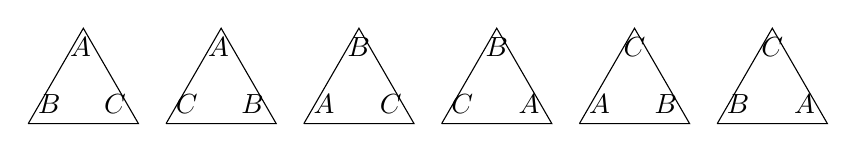
\begin{tikzpicture}[scale=0.7]
              \draw (-1,0)--(1,0)--(0,1.732)--(-1,0);
              \draw (-3.5,0)--(-1.5,0)--(-2.5,1.732)--(-3.5,0);
              \draw (-6,0)--(-4,0)--(-5,1.732)--(-6,0);
              \draw (4,0)--(6,0)--(5,1.732)--(4,0);
              \draw (1.5,0)--(3.5,0)--(2.5,1.732)--(1.5,0);
              \draw (6.5,0)--(8.5,0)--(7.5,1.732)--(6.5,0);
              \node[below] at (-5.05, 1.732) {$A$};
              \node[below] at (-2.55, 1.732) {$A$};
              \node[below] at (-0, 1.732) {$B$};
              \node[below] at (2.5, 1.732) {$B$};
              \node[below] at (5, 1.732) {$C$};
              \node[below] at (7.5, 1.732) {$C$};
              \node[above right] at (-6,0) {$B$};
              \node[above right] at (-3.5,0) {$C$};
              \node[above right] at (-1,0) {$A$};
              \node[above right] at (1.5,0) {$C$};
              \node[above right] at (4,0) {$A$};
              \node[above right] at (6.5,0) {$B$};
              \node[above left] at (-4.05,0) {$C$};
              \node[above left] at (-1.55,0) {$B$};
              \node[above left] at (0.95,0) {$C$};
              \node[above left] at (3.45,0) {$A$};
              \node[above left] at (5.95,0) {$B$};
              \node[above left] at (8.45,0) {$A$};
          \end{tikzpicture}
          \end{center}
          \item Dih$(4)$ is the group of all rotations and reflections that preserve the structure of the regular tetrahedron in $\mathbb{R}^{3}$. An incorrect, yet somewhat useful, way of visualizing this group is to imagine a square in $\mathbb{R}^{2}$. However, the points are not pairwise equidistant and therefore does not preserve symmetry between all points.
          \item Dih$(n)$ is similarly the group of all rotations and reflections that preserve the structure of a regular $(n-1)$-simplex in $\mathbb{R}^{n}$. 
        \end{enumerate}
      \end{example}

  \subsection{Direct Product of Groups}

    \begin{definition}
      The \textit{direct product} of two groups $G$ and $H$ is denoted
      \begin{equation}
        G \times H \equiv \{ (g, h)\;|\; g \in G, h \in H \}
      \end{equation}
      Note that the product need not be binary (nor must it be of finite arity). 
    \end{definition}

    \begin{definition}
      The \textit{general affine group} is defined 
      \begin{equation}
        \text{GA}(V) \equiv \text{Tran}\,V \times \text{GL}(V)
      \end{equation}
    \end{definition}

    \begin{definition}
      The \textit{Galileo Group} is the transformation group of spacetime symmetries that are used to transform between two reference frames which differ only by constant relative motion within the constructs of Newtonian physics. It is denoted 
      \begin{equation}
        \text{Tran}\;\mathbb{R}^{4} \times H \times \text{O} (3)
      \end{equation}
      where $H$ is the group of transformations of the form 
      \begin{equation}
        (x, y, z, t) \longmapsto (x+at, y+bt, z+ct, t)
      \end{equation}
    \end{definition}

    \begin{definition}
      The \textit{Poincaré Group} is the symmetry group of spacetime within the principles of relativistic mechanics, denoted
      \begin{equation}
        G = \text{Tran}\; \mathbb{R}^{4} \times \text{O}_{3,1}
      \end{equation}
      where O$_{3,1}$ is the group of linear transformations preserving the polynomial 
      \begin{equation}
        x^{2} + y^{2} + z^{2} - t^{2}
      \end{equation}
    \end{definition}

  \subsection{Generating Sets and Group Presentations}

    \subsubsection{Cyclic Groups}

      \begin{definition}
        A \textit{word} is any written product of group elements and inverses. They are generally in the form
        \begin{equation}
          s_{1}^{\epsilon_{1}} s_{2}^{\epsilon_{2}} s_{3}^{\epsilon_{3}}... s_{k}^{\epsilon_{k}}
        \end{equation}
      \end{definition}

      \begin{example}
        Given a set $\{x,y,z\}$, $x y, x z^{-1} y y x^{-2},...$ are words. 
      \end{example}

      \begin{definition}
        The \textit{generating set} $\langle S \rangle$ of a group $G$ is a subset of $G$ such that every element of the group can be expressed as a word of finitely many elements under the group operations. The elements of the generating set are called \textit{generators}.
      \end{definition}

      \begin{definition}
        A \textit{cyclic group}, denoted $C_{n}$, is a group generated by a single element. In a \textit{finite cyclic group}, there exists a $k \in \mathbb{N}$ such that $g^{k} = g^{0} = 1$ (or in additive notation, $kg = 0g = 0$), where $g$ is the generator. A \textit{finitely generated group} is a group generated by a finite number of elements. In \textit{infinite cyclic groups}, all elements are distinct for distinct $k$. 
      \end{definition}

      \begin{example}
        A representation of a cyclic group of $n$th order is the $n$th roots of unity in $\mathbb{C}$.
      \end{example}

      \begin{example}
        Another representation of a cyclic group of $n$th order is the set of discrete angular rotations in $SO(2)$, in the form of 
        \begin{equation}
          R =  \bigg\{ \begin{pmatrix}
          \sin{\theta} & \cos{\theta} \\
          \cos{\theta} & -\sin{\theta}
          \end{pmatrix}\; \bigg| \; \theta \in \Big\{\frac{2 \pi}{n} k\Big\}_{k = 0}^{n-1} \bigg\}
        \end{equation}
      \end{example}

      \begin{example}
        $\mathbb{Z}$ is an infinite cyclic group with generator $1$. Furthermore, $\mathbb{Z}/m\mathbb{Z}$ is a finite cyclic group with generator $1$. In fact, the generator of $\mathbb{Z}/m\mathbb{Z}$ can be any integer relatively prime to $m$ (and less than $m$). \end{example}

      \begin{example}
        The set of all \textit{transpositions} forms a generating set of $S_{n}$. 
      \end{example}

      It is actually a fact that every finite cyclic group of order $m$ is isomorphic to $\mathbb{Z}/m\mathbb{Z}$. Every infinite cyclic group is isomorphic to $\mathbb{Z}$. This implies that any two cyclic group of the same order are isomorphic, since we can define a mapping $f:a\longrightarrow b$, where $a$ and $b$ are generating elements of their respective groups. 

      \begin{example}
        Dih$(3) \simeq S_{3}$, since permutations of the vertices of a triangle are isomorphic to a permutations of a 3-element set. 
      \end{example}

      \begin{definition}
        The \textit{free group} $F_{S}$ over a given set $S$ consists of all words that can be built from elements of $S$. Clearly, $S$ is the generating set of $F_{S}$. 
      \end{definition}

    \subsubsection{Group Presentations}

      One method of specifying a group is to put it in the form
      \begin{equation}
        \big\langle \; S \; | \; R \;\big\rangle
      \end{equation}
      where $S$ is the generating set and $R$ is a set of relations. 

      \begin{example}
        The cyclic group of order $n$ could be presented as
        \begin{equation}
          \big\langle \; a \; | \; a^{n} = 1 \;\big\rangle
        \end{equation}
      \end{example}

      \begin{example}
        Dih $(8)$, with $r$ representing a rotation by $45$ degrees in the direction of the orientation and $f$ representing a flip over any axis, is presented by
        \begin{equation}
          \big\langle \; \{ r, f\} \; | \; r^{8} = 1, f^{2} = 1, (r f)^{2} = 1 \;\big\rangle
        \end{equation}
      \end{example}

  \subsection{Cayley's Theorem}

    \begin{lemma}
      Let $G$ be a group with $a \in G$. We define the map
      \begin{equation}
        \phi: G \longrightarrow G, \; \phi (x) = a x a^{-1}
      \end{equation}
      Then, $\phi$ is an automorphism of $G$. 
    \end{lemma}
    \begin{proof}
      The map $\psi: G \longrightarrow G, \; \psi(x) = a^{-1} x a$ is clearly the inverse of $\phi$, with $\phi \psi = \psi \phi = I$ for all $x \in G \implies \phi$ is bijective. Secondly, $\phi(x) \phi(y) = a x a^{-1} a y a^{-1} = a (x y) a ^{-1} = \phi (x y) \implies \phi$ preserves the group structure. 
    \end{proof}

    \begin{theorem}[Cayley's Theorem]
      Every group $G$ is isomorphic to a subgroup of its symmetric group. If $G$ is finite, then so is Sym$(G)$, so every finite group is a subgroup of $S_{n}$, for some $n$.
    \end{theorem}
    \begin{proof}
      Let $H =$ Sym$(G)$. We define the map
      \begin{equation}
        \phi: G \longrightarrow H
      \end{equation}
      by the following rule. For $a \in G$, map it to permutation $\sigma = \phi (a) \in H$ defined as $\sigma(g) = a g$ for all $g \in G$. Note that given an $a \in G$, $a g$ must also be in $G$, meaning that a corresponding $\sigma \in H$ exists. It is sufficient to prove that $\phi$ is an isomorphism onto its image. We first prove injectivity. Given $a \neq b \in G$, $\phi(a)=\sigma, \phi(b) = \tau$. Assume $\sigma = \tau \implies a = a e =  \sigma(e) = \tau (e) = b e = b \implies a = b$, a contradiction. We now check that $\phi(a b) = \phi(a) \phi(b)$. Given $g \in G, \phi(a) \phi(b) (g) = \phi(a) (bg) = a(bg)= (ab) g = \phi(ab) (g).$
    \end{proof}

  \subsection{Group Actions}

    \begin{definition}
      Let $G$ be a group, $X$ a set. Then, a (left) group action of $G$ on $X$ is a function: 
      \begin{equation}
        \varphi: G \times X \longrightarrow X, \; (g,x) \longmapsto \varphi(g,x)
      \end{equation}
      satisfying two axioms:
      \begin{enumerate}
        \item Identity. $\forall x \in X, \varphi(e, x) = x$. 
        \item Compatibility. $\forall g, h \in G \text{ and } \forall x \in X, \varphi(gh, x) = \varphi(g, \varphi(h, x))$.
      \end{enumerate}
      The group $G$ is said to \textit{act on} $X$. $X$ is called a \textit{G-set}. The two axioms, furthermore, imply that for every $g \in G$, the function that maps $x \in X$ to $ \varphi(g, x) \in X$ is a bijective map, since the inverse is the function mapping $x \mapsto \varphi(g^{-1}, x)$. \\
      $(g, x)$ can be interpreted as the element $g$ in the transformation group $G$ acting on an element $x$ in $X$.
    \end{definition}

    \begin{example}
      Isom$\,\mathbb{R}^{3}$ acts on $\mathbb{R}^{3}$ since every element $g \in$ Isom$\,\mathbb{R}^{3}$ acts on the entire space $\mathbb{R}^{3}$. 
    \end{example}

    \begin{example}
      $S_n$ acts on $\{1, 2, ..., n\}$by permuting its elements.
    \end{example}

    \begin{example}
      The GA$(V)$ acts transitively on the points of an affine space.
    \end{example}

    \textbf{Equivalent Interpretation of Group Actions}
    Note that this group action $G$ on space $X$ identifies a group homomorphism into the group of automorphisms of that space. Given an abstract group element $g \in G$, $\varphi(g, \cdot): X \longrightarrow X$ is defined accordingly, where $\varphi(g, \cdot) \in $ Aut$(X)$. So alternatively, we can interpret a group action as a homomorphism from $G$ to Aut$(X)$. 
    \begin{equation}
      \phi: G \longrightarrow \text{Aut}(X), \; g \mapsto \phi(g) = \varphi(g,\cdot)
    \end{equation}

    \begin{definition}
      A group action on a finite-dimensional vector space $X$ is called a \textit{representation} of that group. 
    \end{definition}

  \subsection{Equivalence and Congruence}

    \begin{definition}
      A transformation group $G$ is called \textit{transitive} if for any $x, y \in X$, there exists a $\phi \in G$ such that $y = \phi(x)$. 
    \end{definition}

    \begin{example}
      Tran$(V)$ and GA$(V)$ are transitive groups. 
    \end{example}

    \begin{definition}
      Let $X$ be a set and $G$ its transformation group on $X$. The way we define $G$ determines the \textit{geometry} of $X$. More specifically, a figure $F_{1} \subset X$ is \textit{equivalent} or \textit{congruent} to $F_{2} \subset X$ iff there exists $\phi \in G$ such that $F_{2} = \phi (F_{1})$ (or equivalently, $F_{1} = \phi (F_{2})$). This is an equivalence relation since
      \begin{enumerate}
        \item $F \sim F$. 
        \item $F \sim H \implies H \sim F$. 
        \item $F \sim H, H \sim K \implies F \sim K$
      \end{enumerate}
      Two figures that are in the same equivalence class are known to be \textit{congruent} with respect to the geometry of $X$ induced by $G$. 
    \end{definition}

    Clearly, if two figures are congruent in Euclidean geometry, then they are congruent in Affine geometry, since E$(n) \subset$ GA$(n)$. 

  \subsection{Cosets and Lagrange's Theorem}

    \begin{definition}
      Given a group $G$ and a subgroup $H$, $g_1$ and $g_2$ are congruent modulo $H$, denoted $g_1 \equiv g_2 \pmod{H}$. The equivalence classes are known as \textit{cosets}. A coset of somprised of all the products obtained by multiplying each element of $H$ by a particular element in $G$. Since group multiplication is not necessarily commutative, we must distinguish between right and left cosets. 
      \begin{enumerate}
        \item A \textit{left coset} is 
          \begin{equation}
            g H \equiv \{g h \;| \;h \in H \} 
          \end{equation}
        \item A \textit{right coset} is 
          \begin{equation}
            H g \equiv \{h g \;|\; h \in H \}
          \end{equation}
      \end{enumerate}
      It is easy to see that the cosets form a partition of the set $X$, with each coset of the same cardinality. 
    \end{definition}

    \begin{definition}
      A subgroup $N \subset G$ is a \textit{normal subgroup} iff the left cosets equal the right cosets. Every subgroup of an abelian group is normal. 
    \end{definition}

    \begin{theorem}[Lagrange's Theorem]
      Let $G$ be a finite group and $H$ its subgroup. Then 
      \begin{equation}
        |G| = |G:H| |H|
      \end{equation}
      where $|G:H|$ is the number of cosets in $G$. 
    \end{theorem}

    \begin{corollary}
      The order of a subgroup of a finite group divides the order of the group. 
    \end{corollary}

    \begin{definition}
      The order of an element is the order of the cyclic subgroup that it generates. 
    \end{definition}

    \begin{corollary}
      The order of any element of a finite group divides the order of the group. 
    \end{corollary}

    \begin{corollary}
      Every finite group of a prime order is cyclic. 
    \end{corollary}

    \begin{theorem}[Fermant's Little Theorem]
      Let $p$ be a prime number. The multiplicative group $\mathbb{Z}_{p} \setminus \{0\}$ of the field $\mathbb{Z}_{p}$ is an abelian group of order $p-1 \implies g^{p-1} = 1$ for all $g \in \mathbb{Z}_{p} \setminus \{0\}$. So,
      \begin{equation}
        a^{p-1} \equiv 1 \iff a^{p} \equiv a \pmod{p}
      \end{equation}
    \end{theorem}

    \begin{corollary}
      If $|G| = n$, then $g^{n} = e$ for all $g \in G$. 
    \end{corollary}

    \begin{definition}
      \textit{Euler's Totient Function}, denoted $\varphi(n)$, consists of all the numbers less than or equal to $n$ that are coprime to $n$. 
    \end{definition}

    \begin{theorem}[Euler's Theorem (Generalization of Fermant's Little Theorem)]
      For any $n$, the order of the group $\mathbb{Z}_{n} \setminus \{0\}$ of invertible elements of the ring $\mathbb{Z}_{n}$ equals $\varphi(n)$, where $\varphi$ is Euler's totient function. In other words with $G = \mathbb{Z}_{n} \setminus \{0\}$, 
      \begin{equation}
        a^{\varphi(n)} \equiv 1 \pmod{n}, \; \text{ where $a$ is coprime to $n$}
      \end{equation}
    \end{theorem}

    \begin{example}
      In $\mathbb{Z}_{125} \setminus \{0\}$, $\varphi(125) = 125 - 25 = 100 \implies 2^{100} \equiv 1 \pmod{125}$
    \end{example}

    \begin{definition}
      Let $G$ be a transformation group on set $X$. Points $x, y \in X$ are equivalent with respect to $G$ if there exists an element $g \in G$ such that $y = g x$. This has already been defined through the equivalence of figures before. This relation splits $X$ into equivalence classes, called \textit{orbits}. Note that cosets are the equivalence classes of the transformation group $G$; oribits are those of $X$. We denote it as
      \begin{equation}
        Gx \equiv \{ g x \;|\;g \in G \}
      \end{equation}
    \end{definition}

    By definition, transitive transformation groups have only one orbit.

    \begin{definition}
      The subgroup $G_{x} \subset G$, where $G_{x} \equiv \{ g \in G | g x = x\}$ is called the \textit{stabilizer} of $x$.
    \end{definition}

    \begin{example}
      The orbits of $O(2)$ are concentric circles around the origin, as well as the origin itself. The stabilizer of the point $p \neq 0$ is the identity and the reflection across the line $??$. The stabilizer of $0$ is the entire $O(2)$.
    \end{example}

    \begin{example}
      The group $S_n$ is transitive on the set $\{1, 2, ..., n\}$. The stabilizer of $k, (1 \leq k \leq n)$ is the subgroup $H_{k} \simeq S_{n-1}$, where $H_k$ is the permutation group that does not move $k$ at all. 
    \end{example}

    \begin{theorem}
      There exists a 1-to-1 injective correspondence between an orbit $G_x$ and the set $G / G_{x}$ of cosets, which maps a point $y = g x \in G x $ to the coset $g G_x$. 
    \end{theorem}

    \begin{definition}
      The \textit{length of an orbit} is the number of elements in it. 
    \end{definition}

    \begin{corollary}
      If $G$ is a finite group, then 
      \begin{equation}
        |G| = |G_x| |G x|
      \end{equation}
      In fact, there exists a precise relation between the stabilizers of points of the same orbit, regardless of $G$ being finite or infinite: 
      \begin{equation}
        G_{g x} = g G_{x} g^{-1}
      \end{equation}
    \end{corollary}

  \subsection{Abelian Groups}

    First, note that the successive addition of elements of an additive abelian group can be represented by integer multiplication. 
    \begin{equation}
      x + x + ... + x = n x, \; n \in \mathbb{Z}
    \end{equation}
    Similarly, we can take the integer power of an element to represent successive multiplication in a multiplicative abelian group. 

    \begin{proposition}
      It is easy to check that in an additive abelian group $A$, with $a, b \in A$ and $k, l \in \mathbb{Z}$, 
      \begin{align}
        & k (a + b) = k a + k b \\
        & (k + l) a = k a + l a \\
        & (k l) a = k (l a)
      \end{align}
      which implies
      \begin{equation}
        k(a - b) = k a - k b, \; (k - l) a = k a - l a
      \end{equation}
    \end{proposition}

    \begin{definition}
      For any subset $S \subset A$, the collection of all linear combinations 
      \begin{equation}
        k_1 a_1 + k_2 a_2 + ... + k_n a_n, \; k_i \in \mathbb{Z}, a_i \in S
      \end{equation}
      is the smallest subgroup of $A$ containing $S$, called the \textit{subgroup generated by $S$} and denoted $\langle S \rangle$. If $\langle S \rangle = A$, then we say that $A$ is \textit{generated} by $S$, or that $S$ is a \textit{generating set} of $A$. 
    \end{definition}

    \begin{definition}
      An abelian group that has a finite generating set is called \textit{finitely generated}. Finitely generated abelian groups are similar to finite dimensional vector spaces. 
    \end{definition}

    \begin{definition}
      A system $\{ a_1, a_2, ..., a_n\}$ of elements of a group $A$ is called \textit{linearly independent} if $k_1 a_1 + k_2 a_2 + ... + k_n a_n = 0 \implies k_1, k_2, ..., k_n = 0$. A system of linear independent elements that generates $A$ is called a \textit{basis}. 
    \end{definition}

    Note that every finite dimensional vector has a basis, but not every finitely generated abelian group has one. For example, $(\mathbb{Z}_n, +)$ is generated by one element, but it has no basis since every element $a \in \mathbb{Z}_n$ satisfies the nontrivial relation $n a = 0$. 

    \begin{definition}
      A finitely generated abelian group is \textit{free} if it has a basis. 
    \end{definition}

    \begin{theorem}
      All bases of a free abelian group $L$ contain the same number of elements. 
    \end{theorem}

    \begin{definition}
      The \textit{rank} of a free abelian group $L$ is the number of elements in its basis. It is denoted rk$L$. The zero group is regarded as a free abelian group of rank $0$. 
    \end{definition}

    \begin{theorem}
      Every free abelian group $L$ of rank $n$ is isomorphic to the group $\mathbb{Z}^n$ of integer rows of length $n$. 
    \end{theorem}

    \begin{theorem}
      Every subgroup $n$ of a free abelian group $l$ of rank $n$ is a free abelian group of rank $ \leq n$. 
    \end{theorem}

    Note that unlike a vector space, a free abelian group of positive rank contains subgroups of the same rank that do not conside with the whole group. For example, the subgroup $m \mathbb{Z} \subset \mathbb{Z}, m > 0$ has rank $1$, just as the whole group. 

    Moreover, a free abelian group of rank $n$ can be embedded as a subgroup into an $n$-dimensional Euclidean vector space $E^n$. To do this, let $\{e_1, e_2, ..., e_n\}$ be a basis of $E^n$. Then, the subgroup generated by these basis vectors is the set of vectors with integer components, which is a free abelian group of rank $n$. This subgroup obtained as such is called a \textit{lattice} in $E^n$. 

    \begin{definition}
      A subgroup $L \subset E^n$ is \textit{discrete} if every bounded subset of $E^n$ contains a finite number of elements in $L$. Clearly, every lattice is discrete, and a subgroup generated by a linearly independent system of vectors (i.e. a lattice in a subspace of $E^n$) is discrete. 
    \end{definition}

    \begin{proposition}
      A subgroup $L \subset E^n$ is discrete if and only if its intersection with any neighborhood of $0$ consists of $0$ itself. 
    \end{proposition}

    \begin{theorem}
      Every discrete subgroup $L \subset E^n$ is generated by a linearly independent system of vectors of $E^n$. 
    \end{theorem}

    \begin{corollary}
      A discrete subgroup $L \subset E^n$ whose linear span coincides with $E^n$ is a lattice in $E^n$. 
    \end{corollary}

    Lattices in $E^3$ play an important role in crystallography since the defining feature of a crystal structure is the periodic repetition of the configuration of atoms in all three dimensions. More explicitly, let $\Gamma$ be the symmetry group of the crystal structure and let $\mathcal{L}$ be the group of all vectors $a$ such that the parallel translation $t_a \in \Gamma$. Then, $\mathcal{L}$ is a discrete subgroup of $E^n$ and thus, is a lattice in $E^3$. More specifically, we can present 
    \begin{equation}
      \Gamma \equiv \text{Dih}\,C \times \mathcal{L}
    \end{equation}
    where Dih$\, C$ is the Dihedral group of the crystal structure that preserves its lattices. 

    \begin{definition}
      An \textit{integral elementary row transformation} of a matrix is a transformation of one of the following three types: 
      \begin{enumerate}
        \item adding a row multiplied by an integer to another row
        \item interchanging two rows
        \item multiplying a row by $-1$ 
      \end{enumerate}
      An \textit{integral elementary column transformation} is defined similarly. 
    \end{definition}

    \begin{proposition}
      Every integral rectangular matrix $C = (c_{i j})$ can be reduced by integral elementary row transformations to the diagonal matrix diag$(u_1, ..., u_p)$, where $u_1, u_2, ..., u_p \geq 0$ and $u_i | u_{i+1}$ for $i = 1, 2, ..., p -1$. 
    \end{proposition}

    \begin{example}
      The following matrix can be reduced (with a few steps now shown) to the stated form. 
      \begin{equation}
      \begin{pmatrix} 2&6&2 \\ 2&3&4 \\ 4&2&4 \end{pmatrix} \rightarrow 
      \begin{pmatrix} 2&3&4 \\ 0&-3&2 \\ 4&2&4 \end{pmatrix} \rightarrow
      \begin{pmatrix} 1&0&0 \\ 0&6&14 \\ 0&8&12 \end{pmatrix} \rightarrow
      \begin{pmatrix} 1&0&0 \\ 0&2&0 \\ 0&0&20\end{pmatrix}
      \end{equation}
      where $1|2$ and $2|20$. 
    \end{example}

    Note that for $n \times 1$ or $1 \times n$ matrices, this procedure is precisely the Euclidean algorithm that produces the GCD of $n$ integers. 

    \begin{proposition}
      Given square integral matrix $C$ with  reduced form diag$(u_1, ..., u_p)$, 
      \begin{equation}
        u_i = \frac{d_i}{d_{i-1}}
      \end{equation}
      where $d_i$ is the GCD of the minors of order $i$ of the original matrix $C$. Recall that a minor of a matrix is the determinant of the matrix with one of its rows and columns removed. $d_0$ is assumed to equal $1$. This implies that the numbers $u_1, u_2, ..., u_p$, along with the reduced form, are uniquely determined by $C$. 
    \end{proposition}

    \begin{theorem}
      For any subgroup $N$ of a free abelian group $L$ of rank $n$, there exists a basis $\{e_1, ..., e_n\}$ of $L$ and natural numbers $u_1, ..., u_m, \; (m \leq n)$, such that $\{u_1 e_1, ..., u_m e_m\}$ is a basis fo the group $N$ and $u_i | u_{i+1}$ for $i = 1, 2, ..., m-1$. 
    \end{theorem}

\section{Ring Theory}

  \subsection{Field of Complex Numbers}

    The impossibility of defining division on the ring of integers motivates its extension into the field of rational numbers. Similarly, the inability to take square roots of negative real numbers forces us to extend the field of real numbers to the bigger field of complex numbers. 

    \begin{definition}
      The \textit{field of complex numbers} is a field $\mathbb{C}$ such that 
      \begin{enumerate}
        \item It contains the field $\mathbb{R}$ as a subfield. 
        \item It contains an element $i$ such that $i^2 = -1$.
        \item It is minimal with respect to properties (i) and (ii). That is, if $F$ is a subfield of $\mathbb{C}$ containing $\mathbb{R}$ and $i$, then $F = \mathbb{C}$. 
      \end{enumerate}
    \end{definition}

    Note that the identity $x^2 + 1 \equiv (x + i) (x - i)$ implies that the equation $x^2 = -1$ has exactly two solutions in $\mathbb{C}$, $i$ and $-i$. Therefore, if a subfield of $\mathbb{C}$ contains one of these solutions, it must contain the other (since $i$ and $-i$ are additive and multiplicative inverses). 

    Furthermore, since $i$ is defined to be $\sqrt{-1}$, we could replace $i$ with $-i$ and our calculations would still be consistent throughout the rest of mathematics. In fact, $i$ and $-i$ behave \textit{exactly} identically and cannot be distinguished in an abstract sense. Visually, the complex plane "flipped" across the real number axis produces the same complex plane. 

    \begin{theorem}
      $\mathbb{C}$ exists and is unique up to an isomorphism that maps all real numbers to themselves. Every complex number can be uniquely written as $a + bi$, where $a, b \in \mathbb{R}$ and $i$ is a fixed element such that $i^2 = -1$. 
    \end{theorem}
    \begin{proof}
      We first assume that $\mathbb{C}$ exists. Consider the subset of $\mathbb{C}$
      \begin{equation}
        K \equiv \{ a + bi \; | \; a, b \in \mathbb{R}\}
      \end{equation}
      By evaluating its operations, we can check for closure, identity, and invertibility of nonzero elements to conclude that $K$ is a subfield of $\mathbb{C} \implies$ by prop. (iii), $K = \mathbb{C} \implies$ every element in $\mathbb{C}$ can be written in form $a + bi$. To prove uniqueness, we assume that $p \in \mathbb{C}$ can be written in distinct forms $p = a + bi = a^{\prime} + b^\prime i$. Then
      \begin{align*}
         a + bi = a^{\prime} + b^\prime i & \implies (a - a^\prime)^2 = (b^\prime i - b i)^2 = - (b^\prime - b)^2 \\
         & \implies a - a^\prime = b^\prime - b = 0
      \end{align*}
      To prove uniqueness of $\mathbb{C}$ up to ismorphism, we assume that $\mathbb{C}^\prime$ exists with $i^\prime$ such that $i^{\prime 2}$ containing elements $a + b i'$. Let $f: \mathbb{C} \longrightarrow \mathbb{C}^\prime$ defined 
      \begin{equation}
        f( a + bi) = a + bi^\prime
      \end{equation}
      Then, 
      \begin{align*}
        f\big((a + b i) + (c + d i) \big) & = f\big( (a + c) + (b + d)i \big) \\
        & = (a + c) + (b + d) i^\prime \\
        & = (a + b i^\prime) + (c + d i^\prime) \\
        & = f(a + b i) + f( c + d i) \\
        f\big( \kappa (a + b i)\big) & = f\big( \kappa a + \kappa b i\big) \\
        & = \kappa a + \kappa b i^\prime \\
        & = \kappa (a + b i^\prime) \\
        & = \kappa f(a + b i)
      \end{align*}
      So, $f$ is an isomorphism, and $\mathbb{C} \simeq \mathbb{C}^\prime$. From analysis, we can construct and prove the existence of $\mathbb{R}$. We then define the map
      \begin{equation}
        \rho: \mathbb{R}^2 \longrightarrow \mathbb{C}, \; \rho(a, b) \equiv a + bi
      \end{equation}
      with $\rho(1, 0)$ as the multiplicative identity and $\rho(0,1) \equiv i$. Therefore, every element of $\mathbb{C}$ can be uniquely represented as an element of $\mathbb{R}^2$. 
    \end{proof}

    \begin{definition}
      \textit{Complex conjugation} is an automorphism of $\mathbb{C}$ defined
      \begin{equation}
        c = a + b i \mapsto \bar{c} = a - b i
      \end{equation}
      This is identically defined by replacing $i$ with $-i$. Clearly, $\bar{\bar{c}} = c$. 
    \end{definition}

    \begin{definition}
      Real numbers are elements in $\mathbb{C}$ that are equal to their own conjugates. 
    \end{definition}

    \begin{proposition}
      For any $c \in \mathbb{C}$, $c + \bar{c}$ and $c \bar{c}$ are real. 
    \end{proposition}
    \begin{proof}
      Using the fact that the complex conjugate is an isomorphism, 
      \begin{align*}
        & \bar{c + \bar{c}} = \bar{c} + \bar{\bar{c}} = \bar{c} + c = c + \bar{c} \\
        & \bar{ c \bar{c}} = \bar{c} \bar{\bar{c}} = \bar{c} c = c \bar{c}
      \end{align*}
    \end{proof}
    Note that we proved this abstractly using only the properties given above, and did not decompose $c$ to its \textit{algebraic form} $a + b i$. 

    If $c = a + b i, \; a, b \in \mathbb{R}$, then 
    \begin{equation}
      c + \bar{c} = 2a, \; c \bar{c} = a^2 + b^2
    \end{equation}

    In case the reader is unaware, it is common to interpret complex numbers $c = a + b i$ as points or vectors $(a, b)$ on the complex plane. 

    \subsubsection{Polar Representations of Complex Numbers}

      \begin{definition}
        The \textit{absolute value} of a complex number $c = a + b i$, denoted $|c|$, is the length of the vector representing $c$. 
        \begin{equation}
          |c| \equiv \sqrt{a^2 + b^2}
        \end{equation}
      \end{definition}

      \begin{definition}
        The \textit{argument} of a complex number $c = a + b i$, denoted arg$c$, is the angle formed by the corresponding vector with the polar axis. It is defined within the interval $[0, 2\pi)$. 
        \begin{equation}
          \text{arg}(c) \equiv \tan^{-1}{\frac{b}{a}}
        \end{equation}
      \end{definition}

      \begin{definition}
        The \textit{polar representation}, or \textit{trigonometric representation}, of a complex number $c = a + b i$ is defined using the equations 
        \begin{equation}
          a = r \cos{\varphi}, \; b = r\sin{\varphi} \implies c = r (\cos{\varphi} + i \sin{\varphi})
        \end{equation}
        This mapping can be defined 
        \begin{equation}
          \rho: \mathbb{R} \times \frac{\mathbb{R}}{2 \pi} \longrightarrow \mathbb{C}, \; \rho(r, \varphi) = r (\cos{\varphi} + i \sin{\varphi})
        \end{equation}
      \end{definition}

      \begin{theorem}
        $\rho$ is "similar" to a homomorphism in the following way. By defining the domain and codomain as groups, 
        \begin{equation}
          \rho: \big( \mathbb{R}, \times \big) \times \Big( \frac{\mathbb{R}}{2 \pi} \Big) \longrightarrow \big( \mathbb{C}, \times \big)
        \end{equation}
        we can see that
        \begin{equation}
          \rho (r_1, \varphi_1) \times \rho(r_2, \varphi_2) = \rho(r_1 \times r_2, \varphi_1 + \varphi_2) 
        \end{equation}
        or equivalently, 
        \begin{equation}
          r_1 (\cos{\varphi_1} + i \sin{\varphi_1}) \cdot r_2 (\cos{\varphi_2} + i \sin{\varphi_2}) = r_1 r_2 (\cos{(\varphi_1 + \varphi_2)} + i \sin{(\varphi_1 + \varphi_2)})
        \end{equation}
      \end{theorem}

      \begin{corollary}
        The formula for the ratio of complex numbers is defined
        \begin{equation}
          \frac{r_1 (\cos{\varphi_1} + i \sin{\varphi_1})}{r_2 (\cos{\varphi_2} + i \sin{\varphi_2})} = \frac{r_1}{r_2} (\cos{(\varphi_1 - \varphi_2)} + i \sin{(\varphi_1 - \varphi_2)})
        \end{equation}
      \end{corollary}

      \begin{corollary}
        The positive integer power of a complex number can be written using \textit{De Moivre's formula}. 
        \begin{equation}
          \big(r(\cos{\varphi} + i \sin{\varphi})\big)^n = r^n (\cos{n \varphi} + i \sin{n \varphi})
        \end{equation}
      \end{corollary}

      We can use this formula to extract a root of $n$th degree from a complex number $c = r(\cos{\varphi} + i \sin{\varphi})$, which means to solve the equation $z^n = c$. Let $z = s (\cos{\psi} + i \sin{\psi})$. Then by De Moivre's formula, 
      \begin{align*}
        z^n & = s^n (\cos{n \psi} + i \sin{n \psi}) = r(\cos{\varphi} + i \sin{\varphi}) \\
        & \implies s = \sqrt[n]{r}, \; \psi = \frac{\varphi + 2\pi k}{n} \\
        & \implies z = \sqrt[n]{r} \bigg( \cos{\frac{\varphi + 2\pi k}{n}} + i \sin{\frac{\varphi + 2\pi k}{n}}\bigg) \text{ for } k = 0, 1, ..., n-1
      \end{align*}
      Geometrically, the $n$ solutions lie at the vertices of a regular $n$-gon centered at the origin. When $c = 1$, the solutions are the $n$th roots of unity.

  \subsection{Rings of Residue Class}

    \begin{definition}
      The quotient set $\mathbb{Z}$ by the relation of congruence modulo $n$ is denoted $\mathbb{Z}_{n}$. It is called the \textit{ring of residue class modulo n} or \textit{residue ring modulo n}. 
      \begin{equation}
        \mathbb{Z}_{n} = \{ [0]_{n}, [1]_{n}, ... , [n-1]_{n} \}
      \end{equation}
    \end{definition}

    By definition of the relation, congruence modulo $n$ has properties: 
    \begin{enumerate}
      \item $a \equiv a' \pmod{n}, b \equiv b' \pmod{n} \implies a + b \equiv a' + b' \pmod{n}$ . 
      \item With same hypothesis as (i) $a b \equiv a' b \equiv a b' \equiv a' b' \pmod{n}$. 
    \end{enumerate}
    We can furthermore define operations of addition and multiplication on the ring $\mathbb{Z}_{n}$ as such 
    \begin{align*}
      & [a]_{n} + [b]_{n} \equiv [a + b]_{n} \\
      & [a]_{n} [b]_{n} \equiv [ab]_{n}
    \end{align*}
    making $\mathbb{Z}_{n}$ is a commutative, associative ring with unity. 

    Note that the properties of the operation in $\frac{M}{R}$ inherits all the properties of the addition operation on $M$ that are expressed in the form of identities and inverses, along with the existence of the zero identity. 
    \begin{align*}
      0 \in M & \implies [0] \text{ is the additive identity in } \frac{M}{R} \\
      a + (-a) = 0 & \implies [a] + [-a] = [0] \\
      1 \in M & \implies [1] \text{ is the multiplicative identity in } \frac{M}{R}
    \end{align*}

    \begin{example}
      In $\mathbb{Z}_{5}$, the elements $[2]$ and $[3]$ are multiplicative inverses of each other since $[2] [3] = [6] = [1]$, and $[4]$ is its own inverse since $[4] [4] = [16] = [1]$. The addition and multiplication tables for $\mathbb{Z}_5$ is shown below. 
    \end{example}

    The ring $\mathbb{Z}_n$ has all the properties of a field except the property of having inverses for all of its nonzero elements. This leads to the following theorem. 

    \begin{theorem}
      The ring $\mathbb{Z}_{n}$ is a field if and only if $n$ is a prime number. 
    \end{theorem}
    \begin{proof}
      $(\rightarrow)$ Assume that $n$ is composite $\implies n = k l$ for $k, n \in \mathbb{N} \implies k, n \neq 0$, but 
      \begin{equation}
        [k]_n [l]_n = [k l]_n = [n]_n = 0
      \end{equation}
      meaning that $\mathbb{Z}_n$ contains $0$ divisors and is not a field. The contrapositive of this states $(\rightarrow)$. \\
      $(\leftarrow)$ Given that $n$ is prime, let $[a]_n \neq 0$, i.e. $[a]_n \neq [0]_n, [1]_n$. The set of $n$ elements 
      \begin{equation}
        [0]_n, [a]_n, [2a]_n, ..., [(n-1)a]_n
      \end{equation}
      are all distinct. Indeed, if $[k a]_n = [l a]_n$, then $[(k-l) a]_n = 0 \implies n = (k-l) a \iff n$ is not prime. Since the elements are distinct, exactly one of them must be $[1]_n$, say $[p a]_n \implies$ the inverse $[p]_n$ exists. 
    \end{proof}

    \begin{corollary}
      For any $n$, $[k]_n$ is invertible in the ring $\mathbb{Z}_n$ if and only if $n$ and $k$ are relatively prime. 
    \end{corollary}

    \begin{definition}
      The \textit{characteristic} of ring $R$ (or a field $F$), denoted char$(R)$, is the smallest number of times one must successively add the multiplicative identity $1$ to get the additive identity $0$. That is char$(R)$ is the smallest positive number $n$ such that 
      \begin{equation}
        1 + 1 + ... + 1 = 0 
      \end{equation}
      If no such number $n$ exists, then char$(R) = 0$. The characteristic of $\mathbb{Z}_n = n$
    \end{definition}

    Note that the characteristic of the field $\mathbb{Z}_n$ must be prime. 

    \begin{theorem}[Freshman's Dream]
      Given a field $F$ with char$(F) = p$, 
      \begin{equation}
        (a + b)^p = a^p + b^p
      \end{equation}
    \end{theorem}
    \begin{proof}
      We have 
      \begin{equation}
        (a + b)^p = \sum_{k = 0}^p \binom{p}{k} a^{p-k} b^{k}
      \end{equation}
      It is clear that 
      \begin{equation}
        \binom{p}{k} = \frac{p (p-1) ... (p - k+1)}{k!}
      \end{equation}
      is divisible by $p$ for all $k \neq 0, p$, so all the middle terms must cancel out to $0$. 
    \end{proof}

  \subsection{Polynomial Algebra}

    \subsubsection{Construction and Basic Properties}

      \begin{definition}
        A \textit{polynomial $f$} of $x$ over a ring $R$ is defined as a formal expression 
        \begin{equation}
          f(x) = a_0 + a_1 x^1 + a_2 x^2 + ...  + a_{n-1} x^{n-1} + a_n x^n
        \end{equation}
        where $n$ is a natural number, the coefficients $a_0, a_1, ..., a_n$ are elements of $R$, $x$ is a formal symbol, whose powers $x^i$ are just placeholders for the corresponding coefficients $a_i$ so that the given formal expression is a way to encode the infinite finitary sequence. 
        \begin{equation}
          (a_0, a_1, a_2, ..., a_n, 0, 0, ...)
        \end{equation}
        Two polynomials are equal if and only if the sequences of their corresponding coefficients are equal.
      \end{definition}

      Note that this is really just a fancy way to write a finitary sequence. 

      \begin{definition}
        The set of polynomials with coefficients in the ring $R$ forms itself a ring, called the \textit{ring of polynomials over $R$}, denoted $R[x]$. Addition on $R[x]$ is defined component-wise, and it suffices, by the distributive law, to define multiplication as
        \begin{equation}
          x^k x^l = x^{k + l}
        \end{equation}
        given that we have chosen $\{x^i\}$ as a basis of $R[x]$. If $R$ is a commutative associative ring (or a field), then $R[x]$ is called the \textit{polynomial algebra}. From now, we will treat $R[x]$ and $F[x]$ as an algebra with $R$ denoting a commutative associative ring and $F$ denoting a field, respectively. 
      \end{definition}

      Note that the map from $R \longrightarrow R[x]$ sending $r \mapsto r x^0$ is an injective homomorphism of rings, by which $R$ is viewed as a subring of $R[x]$. 

      The ring of polynomials over field $\mathbb{R}$ is denoted $\mathbb{R}[x]$. $R[x]$ is a subalgebra within the algebra of all function of $\mathbb{R}$. 

      However, for certain finite fields, some formally different polynomials may be indistinguishable in terms of mappings. For example, $x$ and $x^2$ are equivalent in the polynomial algebra defined on the domain $\mathbb{Z}_2$.

      \begin{definition}
        The last nonzero coefficient is called the \textit{leading coefficient}, and the degree of the polynomial $f$, denoted deg$f$, is the index of the leading coefficient. 
      \end{definition}

      \begin{theorem}
      \begin{align}
        \text{deg}(f+g) & \leq \text{max}\{\text{deg}\,f, \text{deg} \,g\} \\
        \text{deg} \,f g & = \text{deg} \,f + \text{deg} \,g
      \end{align}
      \end{theorem}
      \begin{proof}
        Simple when presenting polynomials if form $(1)$. 
      \end{proof}

      \begin{definition}
        The product of two finitary sequences $(a_0, a_1, a_2, ...)$ and $(b_0, b_1, b_2, ...)$ in the ring $F[x]$ is a sequence 
        \begin{equation}
          (c_0, c_1, c_2, ...), \; c_k = \sum_{l = 0}^{k} a_l b_{k-l}
        \end{equation}
        This formula works for infinite (non-finitary) sequences too, allowing us to define a commutative, associative algebra with unity called the \textit{algebra of formal power series over $F$}, denoted $F[[x]]$. The elements of $F[[x]]$ are written in the form 
        \begin{equation}
          a_0 + a_1 x + a_2 x^2 + a_3 x^3...
        \end{equation}
      \end{definition}

      \begin{theorem}
        If the field $F$ is infinite, then different polynomials in $F[x]$ determine different functions. 
      \end{theorem}

      \begin{theorem}
        For any collection of given values $y_1, y_2, ..., y_n \in F$ at given distinct points $x_1, x_2, ..., x_n \in F$, there exists a unique polynomial $f \in F[x]$ with deg$\, f < n$ such that
        \begin{equation}
          f(x_i) = y_i, \; i = 1, 2, ..., n
        \end{equation}
        This is commonly known as the \textit{interpolation problem}, and when $n = 2$, this is called \textit{linear interpolation}. 
      \end{theorem}

      It is usually impossible to divide one polynomial by another in the algebra $F[x]$; the construction of it does not allow us to. However, division \textit{with remainder} is possible, similarly to the procedure of division with remainder in the ring of integers. 

      \begin{theorem}
        Let $f, g \in F[x]$ and $g \neq 0$. Then, there exists polynomials $q, r$ such that 
        \begin{equation}
          f = q g + r, \; \text{deg}\, r < \text{deg}\, g \text{ (or } r = 0 \text{)}
        \end{equation}
        This procedure of finding such polynomials $q, r$ is called \textit{division with a remainder}. A polynomial $f$ is divisible by $g$ in $F[x]$ if and only if $r = 0$. 
      \end{theorem}

      \begin{theorem}[Bezout's Theorem]
        Given that one divides (with remainder) polynomial $f$ by $g = x - c$, let the remainder be $r \in F$. That is, 
        \begin{equation}
          f(x) = (x-c) q(x) + r, \; r \in F
        \end{equation}
        This implies that the remainder equals the value of $f$ at point $c$. That is, 
        \begin{equation}
          f(c) = r
        \end{equation}
      \end{theorem}

    \subsubsection{Roots of Polynomials}

      \begin{definition}
        An element $c \in F$ is a \textit{root} of polynomial $f$ if and only if 
        \begin{equation}
          f(c) = 0
        \end{equation}
      \end{definition}

      \begin{corollary}
        An element $c$ of a field $F$ is a root of polynomial $f$ if and only if $f$ is divisible by $x - c$. 
      \end{corollary}

      \begin{definition}
        A root $c$ of polynomial $f$ is called \textit{simple} if $f$ is not divisible by $(x-c)^2$ and \textit{multiple} otherwise. The \textit{multiplicity} of a root $c$ is the maximum $k$ such that $(x-c)^k$ divides $f$. 
      \end{definition}

      \begin{theorem}
        The number of roots of a polynomial, counted with multiplicity, does not exceed the degree of this polynomial. Furthermore, these numbers are equal if and only if the polynomial is a product of linear factors.
      \end{theorem}

      \begin{definition}
        A \textit{monic polynomial} is a polynomial with leading coefficient equal to $1$. 
      \end{definition}

      \begin{theorem}[Viete's Formulas]
        Given that a polynomial $f$ factors into linear terms, that is 
        \begin{equation}
          f(x) = a_0 \prod_{i = 1}^{n} (x - c_i), c_i \text{ roots of } f
        \end{equation}
        Then the coefficients of $f$ can be presented with the formulas
        \begin{align*}
          & \sum_{i=1}^n c_i = - \frac{a_1}{a_0} \\
          & \sum_{i_1 < i_2} c_{i_1} c_{i_2} = \frac{a_2}{a_0} \\
          & \sum_{i_1< ...< i_k} \prod_{j = 1}^{k} c_{i_j} = (-1)^k \frac{a_k}{a_0} \\
          & c_1 c_2 c_3 ... c_n = (-1)^n \frac{a_n}{a_0}
        \end{align*}
      \end{theorem}

      \begin{theorem}[Wilson's Theorem]
        Let $n$ be a prime number. Then 
        \begin{equation}
          (n-1)! \equiv -1 \pmod{n}
        \end{equation}
      \end{theorem}

      \begin{definition}
        The \textit{derivative} of a polynomial is a map $D: \mathbb{R}[x] \longrightarrow \mathbb{R}[x]$ with the following properties:
        \begin{enumerate}
          \item It is linear. 
          \item $D(f g) = (D f) g + f (D g)$. 
          \item $D x = 1$. 
        \end{enumerate}
      \end{definition}

      In fact, there exists a unique map $D: F[x] \longrightarrow F[x]$ satisfying these properties for any field $F$. 

      \begin{proposition}
        If char$F = 0$, then the coefficients of $f \in F[x]$ regarded as a polynomial in $x - c$ can be expressed as 
        \begin{equation}
          b_k = \frac{ f^{(k)} (c)}{k!}
        \end{equation}
        where $f^{(k)}$ is the $k$th derivative of $f$. 
      \end{proposition}
      \begin{proof}
        We make the substitution $ y = x-c$ in the polynomial $f \in F[x]$ and then express it as a polynomial in $y$ 
        \begin{equation}
          f = b_0 + b_1 (x-c) + b_2 (x-c)^2 + ... + b_n (x-c)^n
        \end{equation}
        We differentiate this equation $k$ times and substitute at $x = c$ to get the corresponding values of the coefficients.
      \end{proof}

    \subsubsection{Fundamental Theorem of Algebra of Complex Numbers}

      While we have defined an upper bound for the number of roots for a polynomial, we have not determined whether a polynomial has any roots at all. Fortunately, it is sufficient to extend the field to $\mathbb{C}$ in order to strongly define a lower limit, too. 

      \begin{definition}
        A field $F$ is \textit{algebraically closed} if every polynomial of positive degree (i.e. non-constant) in $F[x]$ has at least one root in $F$. This is equivalent to saying that every polynomial can be expressed as a product of first degree polynomials.
      \end{definition}

      \begin{proposition}
        A field $F$ is algebraically closed if and only if for each natural number $n$, every endomorphism of $F^n$ (that is, ever linear map from $F^n$ to itself) has at least one eigenvector. 
      \end{proposition}
      \begin{proof}
        An endomorphism of $F^n$ has an eigenvector if and only if its characteristic polynomial has some root. $(\rightarrow)$ So, when $F$ is algebraically closed, every characteristic polynomial, which is an element of $F[x]$, must have a root. $(\leftarrow)$ Assume that every characteristic polynomial has some root, and let $p \in F[x]$. Dividing the polynomial by a scalar doesn't change its roots, so we can assume $p$ to have leading coefficient $1$. If $p(x) = a_0 + a_1 x + ... + x^n$, then we can identify matrix 
        \begin{equation}
          A = \begin{pmatrix}
          0 & 0 & ... & 0 & -a_0 \\
          1 & 0 & ... & 0 & -a_1 \\
          0 & 1 & ... & 0 & -a_2 \\
          ... & ... & ... & ... & ... \\
          0 & 0 & ... & 1 & -a_{n-1}
          \end{pmatrix}
        \end{equation}
        such that the characteristic polynomial of $A$ is $p$. 
      \end{proof}

      \begin{proposition}
        $\mathbb{R}$ is not algebraically closed. 
      \end{proposition}
      \begin{proof}
        $x^2 + 1$ doesn't have any roots in $\mathbb{R}$. 
      \end{proof}

      \begin{theorem}
        Every polynomial of positive degree over field $\mathbb{C}$ has a root. 
      \end{theorem}

      \begin{corollary}
        In the algebra $\mathbb{C}[x]$, every polynomial splits into a product of linear factors. 
      \end{corollary}

      \begin{corollary}
        Every polynomial of degree $n$ over $\mathbb{C}$ has $n$ roots, counted with multiplicities. 
      \end{corollary}

      \begin{corollary}
        $\mathbb{C}$ is algebraically closed. 
      \end{corollary}

    \subsubsection{Roots of Polynomials with Real Coefficients}

      \begin{theorem}
        If $c$ is a complex root of polynomial $f \in \mathbb{R}[x]$, then $\bar{c}$ is also a root of the polynomial. Moreover, $\bar{c}$ has the same multiplicity as $c$. 
      \end{theorem}

      \begin{corollary}
        Every nonzero polynomial in $\mathbb{R}[x]$ factors into a product of linear terms and quadratic terms with negative discriminants. 
      \end{corollary}

      \begin{example}
      \begin{align*}
        x^5 - 1 & = (x-1) \bigg( x - \Big( \cos{\frac{2\pi}{5}} + i \sin{\frac{2\pi}{5}}\Big) \bigg) \bigg( x - \Big( \cos{\frac{2\pi}{5}} - i \sin{\frac{2\pi}{5}}\Big) \bigg) \\
        & \times \bigg( x - \Big( \cos{\frac{4\pi}{5}} + i \sin{\frac{4\pi}{5}}\Big) \bigg) \bigg( x - \Big( \cos{\frac{4\pi}{5}} - i \sin{\frac{4\pi}{5}}\Big) \bigg) \\
        & = (x-1) \bigg( x^2 - \frac{\sqrt{5} - 1}{2} x + 1\bigg) \bigg( x^2 + \frac{\sqrt{5} + 1}{2} x + 1\bigg) 
      \end{align*}
      \end{example}

      \begin{corollary}
        Every polynomial $f \in \mathbb{R}[x]$ of odd degree has at least one real root. 
      \end{corollary}
      \begin{proof}
        This is a direct result of Theorem **. Alternatively, without loss of generality we can assume that the leading coefficient of $f$ is positive. Then
        \begin{equation}
          \lim_{x \rightarrow + \infty} f(x) = + \infty, \; \lim_{x \rightarrow -\infty} f(x) = -\infty
        \end{equation}
        By the intermediate value theorem, there must be some point where $f$ equals $0$. 
      \end{proof}

      \begin{theorem}[Descartes' Theorem]
        The number of positive roots (counted with multiplicities) of a polynomial $f \in \mathbb{R}[x]$ (denote this $N(f)$) does not exceed the number of changes of sign in the sequence of its coefficients (denote this $L(f)$). Additionally, $L(f) \equiv N(f) \pmod{2}$. If all the complex roots of $f$ are real, then $L(f) = N(f)$. 
      \end{theorem}

      Note that if a polynomial has a multiple root but its coefficients are known only approximately (but with any degree of precision), then it is impossible to prove that the multiple roots exists because under any perturbation of the coefficients, however small, it may separate into simple roots or simply cease to exist. This fact leads to the "instability" of the Jordan Normal form because under any perturbation of the elements of a matrix $A$, the change may drastically affect the characteristic polynomial, hence affecting the geometric multiplicities of its eigenvectors. 

    \subsubsection{Factorization in Euclidean Domains}

      Factorization of polynomials over $\mathbb{C}$ into linear factors and polynomials over $\mathbb{R}$ into linear and quadratic factors is similar to the factoring of the integers to prime numbers. In fact, such a factorization exists for polynomials over any field $F$, but their factors can be of any degree. Moreover, there exists no general solution for the factoring of polynomials over any field. 

      \begin{definition}
        A commutative associative ring with unity and without zero divisors is called an \textit{integral domain}. That is, the product of any two nonzero elements $x, y \in A$ must be nonzero. Integral domains are generalizations of the ring of integers $\mathbb{Z}$ and provide a natural setting for studying divisibility. 
      \end{definition}

      \begin{example}
        $\mathbb{Z}$ and $F[x]$ over field $F$ are integral domains. Any field $F$ is also an integral domain. 
      \end{example}

      \begin{example}
        The quotient ring $\mathbb{Z}_n$ is not an integral domain when $n$ is composite. 
      \end{example}

      \begin{example}
        A product of two nonzero commutative rings with unity $R \times S$ is not an integral domain since $(1,0) \cdot (0, 1) = (0, 0) \in R \times S$. 
      \end{example}

      \begin{example}
        The ring of $n \times n$ matrices over any nonzero ring when $ n \geq 2$ is not an integral domain. Given matrices $A, B$, if the image of $B$ is in the kernel of $A$, then $A B = 0$.
      \end{example}

      \begin{example}
        The ring of continuous functions on the interval is not an integral domain. To see why, notice that given the piecewise functions 
        \begin{equation}
          f (x) = \begin{cases}
          1 - 2x & x \in [0, \frac{1}{2}] \\
          0 & x \in [\frac{1}{2}, 1] 
          \end{cases}, \; \;\;g (x) = \begin{cases}
          0 & x \in [0, \frac{1}{2}] \\
          2x - 1 & x \in [\frac{1}{2}, 1] 
          \end{cases}
        \end{equation}
        $f, g \neq 0$, but $f g = g f = 0$. 
      \end{example}

      We can classify the rings
      \begin{equation}
        \text{Integral Domains} \subset \text{Commutative Rings} \subset \text{Rings}
      \end{equation}

      \begin{proposition}
        An integral domain is a ring that is isomorphic to a subring of a field. 
      \end{proposition}

      \begin{proposition}
        The characteristic of an integral domain is either $0$ or a prime number. 
      \end{proposition}

      \begin{definition}
         An element $r$ of a ring $R$ is \textit{regular} if the mapping 
         \begin{equation}
           \rho: R \longrightarrow R, \; x \mapsto x r
         \end{equation}
        is injective for all $x \in R$. 
      \end{definition}

      \begin{proposition}
        An integral domain is a commutative associative ring where every element is regular. 
      \end{proposition}

      \begin{definition}
        Let $A$ be an integral domain. An element $a \in A$ is \textit{divisible} by $b \in A$, denoted $b | a$ if there exists an element $q \in A$ such that $a = q b$. Elements $a$ and $b$ are \textit{associated}, denoted $a \sim b$ if either of the following equivalent conditions holds
        \begin{enumerate}
            \item $a | b \text{ and } b | a$
            \item $a = c b, \text{ where } c$ is invertible
        \end{enumerate}
        The two conditions are equivalent because $c$ and $c^{-1}$ are both in $A$. 
      \end{definition}

      \begin{definition}
        Let $A$ be an integral domain which is not a field. $A$ is \textit{Euclidean} if there exists a function 
        \begin{equation}
          N: A \setminus \{ 0 \} \longrightarrow \mathbb{Z}_+
        \end{equation}
        called a \textit{norm} that satisfies the following conditions. 
        \begin{enumerate}
          \item $N(a b) \geq N(a)$ and the equality holds if and only if $b$ is invertible. 
          \item For any $a, b \in A, \; b \neq 0$, there exist $q, r \in A$ such that $a = q b + r$ with either $r = 0$ or $ N(r) < N(b)$, known as division with remainder. 
        \end{enumerate}
        Uniqueness of $q, r$ is not required in property 2. 
      \end{definition}

      \begin{example}
        The subring of $\mathbb{C}$, defined
        \begin{equation}
          \mathbb{Z}[i] \equiv \{ a + b i \; | \; a, b \in \mathbb{Z} \}
        \end{equation}
        is a Euclidean integral domain with respect to the norm 
        \begin{equation}
          N(c) \equiv a^2 + b^2
        \end{equation}
        since $N(c d) = N(c) N(d)$ and the invertible elements of $\mathbb{Z}[i]$ are $\pm 1, \pm i$. 
      \end{example}

      \begin{example}
        The ring of rational numbers of the form $2^{-n} m, \; n \in \mathbb{Z}_+, m \in \mathbb{Z}$, is a Euclidean domain. To define the norm, we can first assume that $m$ can be prime factorized into the form 
        \begin{equation}
          m = \pm \prod_{i} p_{i}^{k_i}, \; p \text{ prime}
        \end{equation}
        and the norm is defined 
        \begin{equation}
          N(\frac{m}{2^n}) \equiv 1 + \sum_i k_i
        \end{equation}
        We must further show that division with remainder is possible, but we will not show it here. 
      \end{example}

      \begin{definition}
        The \textit{greatest common divisor} of elements $a$ and $b$ of an integral domain is a common divisor of $a$ and $b$ divisible by all their common divisors. It is denoted GCD$(a, b)$. 
      \end{definition}

      \begin{definition}
        A \textit{Gaussian integer} is a complex number whose real part and imaginary part are both integers. That is, 
        \begin{equation}
          \mathbb{Z}[i] \equiv \{a + b i \;|\; a, b \in \mathbb{Z} \}
        \end{equation}
      \end{definition}

    \subsubsection{Polynomials in Several Variables}

      \begin{definition}
        A function of real variable $x_1, x_2, ..., x_n$ is called a \textit{polynomial} if it can be represented as 
        \begin{equation}
          f(x_1, ..., x_n) =  \sum_{k_1, ..., k_n} a_{k_1 ... k_n} x_1^{k_1} x_2^{k_2} ... x_n^{k_n}
        \end{equation}
        where the summation is taken over a finite set of collections $(k_1, ..., k_n)$. The algebra of polynomials in $x_1, x_2, ..., x_n$ over $\mathbb{R}$ is denoted $\mathbb{R}[x_1, x_2, ..., x_n]$. 
      \end{definition}

      \begin{definition}
        More generally, an infinite dimensional polynomial algebra of variables $x_1, ..., x_n$ over field $\mathbb{F}$ is denoted
        \begin{equation}
          \mathbb{F}[x_1, ..., x_n]
        \end{equation}
        Like polynomials of one variable, it can be naturally identified with an abstract multi-dimensional "sequence." It has basis 
        \begin{equation}
          \{e_{k_1 k_2 ... k_n} \;|\; k_1, k_2, ..., k_n \in \mathbb{Z}_+
        \end{equation}
        with addition defined component-wise and the multiplication rule defined with the table
        \begin{equation}
          e_{k_1...k_n} e_{l_1 ... l_n} = e_{k_1 + l_1, k_2 + l_2, ..., k_n + l_n}
        \end{equation}
        Clearly each polynomial in its usual presentation is gotten by the linear mapping
        \begin{equation}
          e_{k_1 ... k_n} \mapsto x_1^{k_1} x_2^{k_2} ... x_n^{k_n}
        \end{equation}
      \end{definition}

      However, note that different polynomials may define the same functions if the field $\mathbb{F}$ is finite, similarly to polynomials with one variable. If $\mathbb{F}$ is infinite, then every polynomial will determine a different function. 

      \begin{definition}
        A polynomial is called \textit{homogeneous} if degree $d$ if 
        \begin{equation}
          a_{k_1 k_2 ... k_n} = 0 \text{ for } k_1 + k_2 + ... + k_n \neq d
        \end{equation}
        The space of all homogeneous polynomials of fixed degree $d$ forms a finite dimensional subspace in $\mathbb{F}[x_1, ..., x_n]$ with dimension 
        \begin{equation}
          \frac{n(n+1)...(n+d-1)}{d!}
        \end{equation}
        The dimension can be calculated by thinking of the combinatorics problem of having $d$ indistinguishable balls to put into $n$ distinguishable urns. 
      \end{definition}

    \subsubsection{Symmetric Polynomials}

      \begin{definition}
        A polynomial $f \in \mathbb{F}[x_1, ..., x_n]$ is called \textit{symmetric} if it is invariant under any permutation of the variables $x_i$. 
      \end{definition}

      \begin{example}
        Power sums are symmetric polynomials. 
        \begin{equation}
          p(x_1, x_2, ..., x_n) = \sum_{i=1}^n x_i^k
        \end{equation}
      \end{example}

      \begin{definition}
        An \textit{elementary symmetric polynomial} is a symmetric polynomial of one of these forms: 
        \begin{align*}
          \sigma_1 & = x_1 + x_2 + ... + x_n \\
          \sigma_2 & = x_1 x_2 + x_1 x_3 + ... + x_{n-1} x_n \\
          ... & = ... \\
          \sigma_k & = \sum_{i_1 < ... < i_k} x_{i_1} x_{i_2} ... x_{i_k} \\
          ... & = ... \\
          \sigma_n & = x_1 x_2 ... x_n
        \end{align*}
      \end{definition}

      The following theorem presents an extremely useful result about the decomposition of symmetric polynomials. 

      \begin{theorem}
        Every symmetric polynomial can be written as a polynomial of elementary symmetric polynomials $\sigma_i$. 
      \end{theorem}

      \begin{example}
        The polynomial 
        \begin{equation}
          f \equiv \sum_{i=1}^n x_i^3
        \end{equation}
        can be expressed as 
        \begin{equation}
          f = \sigma_1^3 - 3 \sigma_1 \sigma 2 + 3 \sigma_3
        \end{equation}
      \end{example}

    \subsubsection{Cubic Equations}

      The well known discriminant of a quadratic equation 
      \begin{equation}
        f(x) = ax^2 + bx + c
      \end{equation}
      is known in the form $\nabla = b^2 - 4ac$. However, we will present it in a slightly different manner. 

      \begin{definition}
        The \textit{discriminant} $D(\varphi)$ of a quadratic polynomial
        \begin{equation}
          \varphi = a_0 x^2 + a_1 x + a_2 \in \mathbb{C}[x]
        \end{equation}
        with $c_1, c_2 \in \mathbb{C}$ as its roots is defined
        \begin{equation}
          D(\varphi) = a_1^2 - 4 a_0 a_2 = a_0^2 \bigg( \Big(\frac{a_1}{a_0} \Big)^2 - \frac{4 a_2}{a_0} \bigg) = a_0^2 \big( (c_1 + c_2)^2 - 4 c_1 c_2 \big) = a_0^2 (c_1 - c_2)^2
        \end{equation}
        Clearly, the value of $D(\varphi)$ can tell us three things
        \begin{enumerate}
          \item $c_1, c_2 \in \mathbb{R}, c_1 \neq c_2$. Then $c_1 - c_2$ is a nonzero real number and $D(\varphi) > 0$. 
          \item $c_1 = c_2 \in \mathbb{R}$. Then $c_1 - c_2 = 0$ and $D(\varphi) = 0$. 
          \item $c_1, c_2 \in \mathbb{C}, c_1 = \bar{c}_2$. Then, $c_1 - c_2$ is a nonzero strictly imaginary number and $D(\varphi) < 0$. 
        \end{enumerate}
      \end{definition}

      \begin{definition}
        We can generalize this notion of the discriminant to arbitrary polynomials
        \begin{equation}
          \varphi = a_0 x^n + a_1 x^{n-1} + ... + a_{n-1} x + a_n \in \mathbb{F}[x], \; a_0 \neq 0
        \end{equation}
        The discriminant $D(\varphi)$ of the polynomial above is defined
        \begin{equation}
          D(\varphi) \equiv a_0^{2n-2} \prod_{i>j} (c_i - c_j)^2
        \end{equation}
        The $a_0$ term isn't very important in this formula, since it does not affect whether $D(\varphi)$ is positive, negative, or zero. 
      \end{definition}

      \begin{definition}
        A polynomial 
        \begin{equation}
          \varphi = a_0 x^n + a_1 x^{n-1} + ... + a_{n-1} x + a_n \in \mathbb{F}[x], \; a_0 \neq 0
        \end{equation}
        where $a_1 = 0$ is called \textit{depressed}. A depressed cubic polynomial is of form
        \begin{equation}
          \varphi = x^3 + p x + q
        \end{equation}
      \end{definition}

      \begin{proposition}
        Every monic (leading coefficeint $=1$) polynomial (and non-monic ones) 
        \begin{equation}
          \varphi = x^n + a_1 x^{n-1} + ... + a_{n-1} x + a_n \in \mathbb{F}[x], \; a_0 \neq 0
        \end{equation}
        can be turned into a depressed polynomial with the change of variable
        \begin{equation}
          x = y - \frac{a_1}{n}
        \end{equation}
        to get the polynomial 
        \begin{equation}
          \psi = y^n + b_2 y^{n-2} + ... + b_{n-1} y + b_n
        \end{equation}
      \end{proposition}

      \begin{lemma}
        A cubic polynomial 
        \begin{equation}
          \varphi = a_0 x^3 + a_1 x^2 + a_2 x + a_3 \in \mathbb{R}[x]
        \end{equation}
        with roots $c_1, c_2, c_3 \in \mathbb{C}$ has discriminant
        \begin{equation}
          D(\varphi) \equiv a_0^4 (c_1 - c_2)^2 (c_1 - c_3)^2 (c_2 - c_3)^2
        \end{equation}
        With a bit of evaluation, it can also be expressed in terms of its coefficients as
        \begin{equation}
          D(\varphi) = a_1^2 a_2^2 - 4a_1^3 a_3 - 4a_0 a_2^3 + 18 a_0 a_1 a_2 a_3 - 27 a_0^2 a_3^2
        \end{equation}
        Again, three possibilities can occur (up to reordering of its roots). 
        \begin{enumerate}
            \item $c_1, c_2, c_3$ are distinct real numbers. Then $D(\varphi) > 0$. 
            \item $c_1, c_2, c_3 \in \mathbb{R}, c_1 = c_2$. Then $D(\varphi) = 0$. 
            \item $c_1 \in \mathbb{R}, c_2 = \bar{c}_3 \not\in \mathbb{R}$. Then $D(\varphi) < 0$. 
        \end{enumerate}
        Furthermore, the cubic formula used to find the roots of the polynomial is 
        \begin{equation}
          c_{1, 2, 3} = \sqrt[3]{-\frac{q}{2} + \sqrt{\frac{p^3}{27} + \frac{q^2}{4}}} + \sqrt[3]{-\frac{q}{2} - \sqrt{\frac{p^3}{27} + \frac{q^2}{4}}}
        \end{equation}
        known as \textit{Cardano's formula}, after the mathematician Gerolamo Cardano. 
      \end{lemma}

  \subsection{Ideals and Quotient Rings}

    \begin{definition}
      For an arbitrary ring $(R,+, \cdot)$, let $(R, +)$ be its additive group. A subset $I$ is called a \textit{left ideal} of $R$ if it satisfies the two conditions. 
      \begin{enumerate}
        \item $(I, +)$ is a subgroup of $(R, +)$. 
        \item For every $r \in R$ and every $x \in I$ the left product $r \cdot x \in I$. 
      \end{enumerate}
      Similarly, a \textit{right ideal} $I$ of $R$ satisfies
      \begin{enumerate}
        \item $(I, +)$ is a subgroup of $(R, +)$. 
        \item For every $r \in R$ and every $x \in I$, the right product $r \cdot x \in I$. 
      \end{enumerate}
      Note that left and right modules are equivalence relations defined on a ring. 
    \end{definition}

    A left/right ideal can also be seen as a left/right $R$-submodule of $R$ viewed as an $R$-module. 

    \begin{definition}
      A \textit{two-sided ideal}, or more simply an \textit{ideal}, is a left ideal that is also a right idea. 
    \end{definition}

    \begin{proposition}
      Every right or left ideal of a commutative ring is a two sided ideal. 
    \end{proposition}
    \begin{proof}
      Trivial. 
    \end{proof}

    \begin{example}
      The set of even integers $2 \mathbb{Z}$ is an ideal in the ring $\mathbb{Z}$, since the sum of any even integers is even and the product of any even integer with an integer is an even integer. However, the odd integers do not form an ideal. 
    \end{example}

    \begin{example}
      The set of all polynomials with real coefficients which are divisible by the polynomial $x^2 + 1$ is an ideal in the ring of all polynomials. 
    \end{example}

    \begin{example}
      The set of all $n \times n$ matrices whose last row is zero forms a right ideal in the ring of all $n \times n$ matrices. However, it is not a left ideal.

      The set of all $n\times n$ matrices whose last column is zero is a left ideal, but not a right ideal. 
    \end{example}

    \begin{proposition}
      The only ideals that exist in a field $\mathbb{F}$ is $\{0\}$ and $\mathbb{F}$ itself. 
    \end{proposition}
    \begin{proof}
      Given a nonzero element $x \in \mathbb{F}$, every element of $\mathbb{F}$ can be expressed in the form of $a x$ or $x a$ for some $a \in \mathbb{F}$. 
    \end{proof}

    \begin{definition}
      A left ideal generated by a single element $x$ is called the \textit{principal left ideal generated by $x$} and is denoted $R x$. Principal right ideals are denoted $x R$, and principal (two-sided) ideals are denoted $R x R$. 
    \end{definition}

    \begin{definition}
      A \textit{principal ideal domain}, also called a \textit{PID}, is an integral domain in which every ideal is principal (i.e. can be generated by a single element). 

      More generally, a \textit{principal ideal ring} is a nonzero commutative ring in which every ideal is principal (i.e. can be generated by a single element). 
    \end{definition}

    The distinction is that a principal ideal ring may have zero divisors whereas a principal ideal domain cannot. Principal ideal domains are thus mathematical objects that behave somewhat like the integers. That is, 
    \begin{enumerate}
      \item Any element of a PID has a unique decomposition into prime elements. 
      \item Any two elements of a PID have a greatest common divisor. 
      \item If $x$ and $y$ are elements of a PID without common divisors, then every element of the PID can be written in the form 
        \begin{equation}
          a x + b y
        \end{equation}
    \end{enumerate}

    \begin{proposition}
      Every Euclidean domain is also a principal ideal domain. 
    \end{proposition}

    \begin{example}
      The following are all examples of principal ideal domains. 
      \begin{enumerate}
        \item Any field $\mathbb{F}$. 
        \item The ring of integers $\mathbb{Z}$. 
        \item $\mathbb{F}[x]$, rings of polynomials in one variable with coefficients in a field $\mathbb{F}$. 
        \item Rings of formal power series $\mathbb{F}[[x]]$. 
        \item The ring of Gaussian integers $\mathbb{Z}[i]$. 
      \end{enumerate}
    \end{example}

    It is quite easy to see that a field $\mathbb{F}$ is a PID since the only two possible ideals are $\{0\}$ and $\mathbb{F}$, both of which are principal. For the integers $\mathbb{Z}$, every ideal is of the form $n\mathbb{Z}$, which is principal since it is generated by the integer $n$. The ring of polynomials $\mathbb{F}[x]$ is a PID since we can imagine a minimal polynomial $p$ in each ideal $I$. Every element in $I$ must be divisible by $p$, which means that the entire ideal $I$ can be generated by the minimal polynomial $p$, making $I$ principal. 

  \subsection{The Algebra of Quaternions}

    \begin{definition}
      The \textit{quaternions} form an algebra of $4$-dimensional vectors over $\mathbb{R}$, with elements of the form
      \begin{equation}
        (a, b, c, d) \equiv a + bi + cj + dk
      \end{equation}
      where $a$ is called the \textit{scalar portion} and $bi + cj + dk$ is called the \textit{vector/imaginary portion}. The algebra of quaternions is denoted $\mathbb{H}$, which stands for "Hamilton." $\mathbb{H}$ is a $4$-dimensional associative normed division algebra over $\mathbb{R}$. 
    \end{definition}

    From looking at the multiplication table, we can see that multiplication in $\mathbb{H}$ is not commutative. 
    \begin{center}
      \begin{tabular}{|c|c|c|c|c|}
      \hline
      i & i & -1 & k & -j \\ 
      \hline
      j & j & -k & -1 & i \\ 
      \hline
      k & k & j & -i & -1 \\ 
      \hline
      \end{tabular}
    \end{center}
    Note the identity 
    \begin{equation}
      i^2 = j^2 = k^2 = -1
    \end{equation}
    The algebra of quaternions are in fact the first noncommutative algebra to be discovered! 

    \begin{proposition}
      $\mathbb{H}$ and $\mathbb{C}$ are the only finite-dimensional divisions rings containing $\mathbb{R}$ as a proper subring. 
    \end{proposition}

    \begin{definition}
      The \textit{quaternion group}, denoted $Q_8$ is a nonabelian group of order $8$, isomorphic to a certain $8$-element subset in $\mathbb{H}$ under multiplication. It's group presentation is 
      \begin{equation}
        Q_8 = \big\langle \bar{e}, i, j, k \;|\; \bar{e}^2 = e, i^2 = j^2 = k^2 = ijk = \bar{e} \big\rangle
      \end{equation}
    \end{definition}

    Going back to the algebra, we can set $\{1, i, j, k\}$ as a basis and define addition and scalar multiplication component-wise, and multiplication (called the \textit{Hamilton product}) with properties
    \begin{enumerate}
      \item The real quaternion $1$ is the identity element. 
      \item All real quaternions commute with quaternions: $a q = q a$ for all $a \in \mathbb{R}, q \in \mathbb{H}$. 
      \item Every quaternion has an inverse with respect to the Hamilton product. 
        \begin{equation}
          (a + bi + cj + dk)^{-1} = \frac{1}{a^2 + b^2 + c^2 + d^2} \big( a - bi - cj - dk\big)
        \end{equation}
    \end{enumerate}
    Note that property 3 allows $\mathbb{H}$ to be a division algebra. 

    \begin{proposition}[Scalar and Vector Components]
      Let the quaternion be divided up into a scalar and vector part with the bjective mapping $a + bi + cj + dk \mapsto \big(a, (b, c, d)\big)$. 
      \begin{equation}
        q = (r, v), r \in \mathbb{R}, v \in \mathbb{R}^3
      \end{equation}
      Then, the formulas for addition and multiplication are
      \begin{align*}
        q_1 + q_2 & = (r_1, v_1) + (r_2, v_2) = (r_1 + r_2, v_1 + v_2) \\
        q_1 \cdot q_2 & = (r_1, v_1) \cdot (r_2, v_2) = (r_1 r_2 - v_1 \cdot v_2, r_1 v_2 + r_2 v_1 + v_1 \times v_2)
      \end{align*}
      where the $\cdot$ and $\times$ on the right hand side represnts the dot product and cross product, respectively. 
    \end{proposition}

    \begin{definition}
      The conjugate of a quaternion $q = a + bi + cj + dk$ is defined 
      \begin{equation}
        \bar{q}, q^* \equiv a - bi - cj - dk
      \end{equation}
      It has properties
      \begin{enumerate}
        \item $q^{**} = q$
        \item $(q p)^* = p^* q^*$
      \end{enumerate}
      $q^*$ can also be expressed in terms of addition and multiplication. 
      \begin{equation}
        q^* = -\frac{1}{2} \big( q + iqi + jqj + kqk \big)
      \end{equation}
    \end{definition}

    \begin{definition}
      The \textit{norm} of $q$ is defined
      \begin{equation}
        ||q|| \equiv \sqrt{q^* q} = \sqrt{q q^*} = \sqrt{a^2 + b^2 + c^2 + d^2}
      \end{equation}
      with properties
      \begin{enumerate}
        \item Scaling factor. $||\alpha q|| = |\alpha| ||q||$
        \item Multiplicative. $||p q|| = ||p|| ||q||$
      \end{enumerate}
    \end{definition}

    The norm allows us to define a metric 
    \begin{equation}
      d(p, q) \equiv ||p - q||
    \end{equation}
    This makes $\mathbb{H}$ a metric space, with addition and multiplication continuous on the metric topology. 

    \begin{definition}
      The \textit{unit quaternion} is defined to be
      \begin{equation}
        U_q = \frac{q}{||q||}
      \end{equation}
    \end{definition}

    \begin{corollary}
      Every quaternion has a polar decomposition
      \begin{equation}
        q = U_q \cdot ||q||
      \end{equation}
      With this, we can redefine the inverse as
      \begin{equation}
        q^{-1} = \frac{q^*}{||q||^2}
      \end{equation}
    \end{corollary}

    \subsubsection{Matrix Representations of Quaternions}

      We can represent $q$ with $2 \times 2$ matrices over $\mathbb{C}$ or $4\times 4 $ matrices over $\mathbb{R}$. 

      \begin{proposition}
        The following representation is an injective homomorphism $\rho: \mathbb{H} \longrightarrow \GL(2, \mathbb{C})$. 
        \begin{equation}
          \rho: a + bi + cj + dk \mapsto \begin{pmatrix}
          a+bi & c+ di \\ -c + di & a - bi
          \end{pmatrix}
        \end{equation}
        It has properties
        \begin{enumerate}
          \item Constraining any two of $b, c, d$ to $0$ produces a representation of the complex numbers. When $c = d = 0$, this is called the \textit{diagonal representation}. 
          \begin{align*}
            \begin{pmatrix}
            a+bi & 0 \\ 0 & a-bi
            \end{pmatrix},  \begin{pmatrix}
            a & c \\ -c & a
            \end{pmatrix},  \begin{pmatrix}
            a & di \\ di & a
            \end{pmatrix}
          \end{align*}
          \item The norm of a quaternion is the square root of the determinant of its corresponding matrix representation. 
            \begin{equation}
              ||q|| = \sqrt{\det \begin{pmatrix}
              a+bi & c+di \\ -c+di & a-bi
              \end{pmatrix}} = \sqrt{(a^2 + b^2) + (c^2 + d^2)}
            \end{equation}
          \item The conjugate of a quaternion corresponds to the conjugate (Hermitian) transpose of its matrix representation. 
            \begin{equation}
              \rho(q^*) = \rho(q)^H \iff a-bi-cj-dk \mapsto \begin{pmatrix}
              a-bi & -c-di \\ c-di & a+bi
              \end{pmatrix}
            \end{equation}
          \item The restriction of this representation to only unit quaternions leads to an isomorphism between the subgroup of unit quaternions and their corresponding image in SU$(2)$. Topologically, the unit quaternions is the $3$-sphere, so the underlying space SU$(2)$ is also a $3$-sphere. More specifically, 
            \begin{equation}
              \frac{\text{SU}(2)}{2} \simeq \text{SO}(3)
            \end{equation}
        \end{enumerate}
      \end{proposition}

      \begin{proposition}
      The following representation of $\mathbb{H}$ is an injective homomorphism $\rho: \mathbb{H} \longrightarrow \GL(4, \mathbb{R})$. 
      \begin{equation}
        \rho: a+bi+cj+dk \mapsto \begin{pmatrix}
        a&-b&-c&-d \\
        b&a&-d&c\\
        c&d&a&-b\\
        d&-c&b&a
        \end{pmatrix}
      \end{equation}
      or also as
      \begin{equation}
        a \begin{pmatrix}
        1 &0 &0 &0 \\
        0& 1&0&0\\
        0&0&1&0\\
        0&0&0&1
        \end{pmatrix} + b \begin{pmatrix}
        0&-1&0&0\\1&0&0&0\\0&0&0&-1\\0&0&1&0
        \end{pmatrix} + c\begin{pmatrix}
        0&0&-1&0\\0&0&0&1\\1&0&0&0\\0&-1&0&0
        \end{pmatrix} + d \begin{pmatrix}
        0&0&0&-1\\0&0&-1&0\\0&1&0&0\\1&0&0&0
        \end{pmatrix}
      \end{equation}
      It has properties
      \begin{enumerate}
        \item $\rho(q^*) = \rho(q)^T$
        \item The fourth power of the norm is the determinant of the matrix 
          \begin{equation}
            ||q||^4 = \det\big( \rho (q)\big)
          \end{equation}
        \item Similarly, with the $2\times 2$ representation, complex number representations can be produced by restricting $2$ of $b, c, d$ to $0$. 
      \end{enumerate}
      \end{proposition}

      Note that this representation in $\GL(4, \mathbb{R})$ is not unique. There are in fact 48 distinct representation of this form where one of the component matrices represents the scalar part and the other 3 are skew symmetric. 

    \subsubsection{Square Roots of -1}

      In $\mathbb{C}$, there are two numbers, $i$ and $-i$, whose square is $-1$. However, in $\mathbb{H}$, infinitely many square roots of $-1$ exist, forming the unit sphere in $\mathbb{R}^3$. To see this, let $q = a+bi+cj+dk$ be a quaternion, and assume that its square is $-1$. Then this implies that
      \begin{equation}
        a^2 - b^2 -c^2 -d^2 = -1, 2ab = 2ac = 2ad = 0
      \end{equation}
      To satisfy the second equation, either $a=0$ or $b=c=d=0$. The latter is impossible since then $q$ would be real. Therefore, 
      \begin{equation}
        b^2 + c^2 + d^2 = 1
      \end{equation}
      which forms the unit sphere in $\mathbb{R}^3$. 

\section{Affine and Projective Spaces}

  \subsection{Affine Spaces}

    Modeling the space of points as a vector space can be unsatisfactory for a number of reasons. 
    \begin{enumerate}
      \item The origin $0$ plays a special role, when it doesn't necessarily need to have one. 
      \item Certain notions, such as parallelism, are handled in an awkward manner. 
      \item The geometries of vector and affine spaces are intrinsically. That is, 
        \begin{equation}
          \GL(V) \subset \GA(V)
        \end{equation}
    \end{enumerate}

    In the ordinary Euclidean geometry, one can define the operation of the addition of a point and a vector. That is, the "sum" of a point $p$ and a vector $x$ is the endpoint of a vector that starts at $p$ and equals $x$. We formalize it in the following definition. 

    \begin{definition}
      Let $V$ be a vector space over field $\mathbb{F}$. The \textit{affine space associated to $V$} is a set $S$ with an operation of addition $+: S \times V \longrightarrow S$ satisfying 
      \begin{enumerate}
        \item $p + (x + y) = (p + x) + y$ for $p \in S, x, y \in V$
        \item $p + 0 = p$ where $p \in S$, $0$ is the zero vector 
        \item For any $p, q \in S$, there exists a unique vector $x$ such that $p + x = q$
      \end{enumerate}
      Elements of the set $S$ are called \textit{points}. The vector in condition 3 is called the \textit{vector connecting points $p$ and $q$}, denoted $\overline{pq}$. The dimension of an affine space is defined as the dimension of the corresponding vector space. 
    \end{definition}

    The first condition implies that
    \begin{equation}
      \overline{pq} + \overline{qr} = \overline{pr} \text{ for all } p, q, r \in S
    \end{equation}
    Every vector space $V$ can be regarded as an affine one if we view vectors both as points and as points and define the operation of addition of a vector to a point as addition of vectors. Under this interpretation, the vector $\overline{pq}$ is the difference between the vectors $p$ and $q$. 

    \begin{definition}
      Conversely, if we fix a point $o$ (the origin) in an affine space $S$, we can identify a point $p$ with its \textit{position vector} $\overline{op}$. Then, addition of a vector to a point just becomes the addition a vectors. This identification of points with vectors is called the \textit{vectorization} of an affine space. 
    \end{definition}

    \begin{definition}
      A point $o$ (the origin) together with a basis $\{e_1, ..., e_n\}$ of the space $V$ is called a \textit{frame} of the affine space $S$. Each frame is related to an \textit{affine system of coordinates} in the space $S$. That is, a point $p$ would get the coordinates equal to those of the vector $\overline{op}$ in the basis $\{e_1, ..., e_n\}$. It is easy to see that 
      \begin{enumerate}
        \item Coordinates of the point $p+x$ are equal to the sums of respective coordinates of the point $p$ and the vector $x$. 
        \item Coordinates of the vector $\overline{pq}$ are equal to the differences of respective coordinates of the points $q$ and $p$. 
      \end{enumerate}
    \end{definition}

    Linear combinations of points are not defined in the affine space since the values of linear combinations are actually dependent on the choice of the origin. However, an analogous structure can be. 

    \begin{definition}
      The \textit{barycentric linear combination} of points $p_1, ..., p_k \in S$ is a linear combination of the form
      \begin{equation}
        p = \sum_i \lambda_i p_i, \text{ where } \sum_i \lambda_i = 1
      \end{equation}
      This linear combination is equal to the point $p$ such that
      \begin{equation}
        \overline{op} = \sum_i \lambda_i \overline{op_i}
      \end{equation}
      where $o \in S$ is any origin point.
    \end{definition}

    \begin{definition}
      In particular, the specific barycentric combination of points where $\lambda_1 = ... = \lambda_k = \frac{1}{k}$ is called the \textit{center of mass} of the collection of points $p_i$. 
    \end{definition}

    \begin{definition}
      Let $p_0, p_1, ..., p_n$ be points of an $n$-dimensional affine space $S$ such that the vectors $\overline{p_0 p_1}, ..., \overline{p_0 p_n}$ are linearly independent (that is, forms a basis). Then, every point $p \in S$ can be uniquely presented as 
      \begin{equation}
        p = \sum_{i=0}^n x_i p_i, \text{ where } \sum_{i=0}^n x_i = 1
      \end{equation}
      This equality can be rewritten
      \begin{equation}
        \overline{p_0 p} = \sum_{i=1}^n x_i \overline{p_0 p_i}
      \end{equation}
      implying that we can take the coordinates of the vector $\overline{p_0 p}$ in the basis $\{ \overline{p_0 p_1}, ..., \overline{p_0 p_n}\}$ as $x_1, ..., x_n$. Then, $x_0$ is determined as 
      \begin{equation}
        x_0 = 1 - \sum_{i=1}^n x_i
      \end{equation}
      The numbers $x_0, x_1, ..., x_n$ are called the \textit{barycentric coordinates} of the point $p$ with respect to $p_0, p_1, ..., p_n$. 
    \end{definition}

    \begin{definition}
      A \textit{plane} in an affine space $S$ is a subset of the form 
      \begin{equation}
        p = p_0 + U
      \end{equation}
      where $p_0$ is a point and $U$ is a subspace of the space $V$. Note that we can choose any point $p_0$ in the plane in this representation. $U$ is called the \textit{direction subspace} for $P$. 
    \end{definition}

    \begin{lemma}
      If the intersection of two planes in an affine space is nonempty, then the intersection is also a plane. 
    \end{lemma}

    \begin{theorem}
      Given any $k+1$ points of an affine space, there is a plane of dimension $\leq k$ passing through these points. If these points are not contained in a plane of dimension $< k$, then there exists a unique $k$-dimensional plane passing through them. 
    \end{theorem}

    \begin{definition}
      Points $p_0, p_1, ..., p_k \in S$ are \textit{affinely dependent} if they lie in a plane of dimension $<k$, and \textit{affinely independent} otherwise. It is clear that the points $p_0,..., p_k$ are affinely independent if and only if the vectors $\overline{p_0p_1}, ..., \overline{p_0 p_k}$ are linearly independent. 
    \end{definition}

    \begin{theorem}
      Points $p_0, ..., p_k \in S$ are affinely independent if and only if the rank of the matrix of their barycentric coordinates (with respect to some predetermined affinely independent points) equals $k+1$. 
    \end{theorem}

    It is easy to see that the previous theorem is true, since the determinant represents the hypervolume of the parallelopiped spanned by the vectors $\overline{p_0p_1}, ..., \overline{p_0 p_k}$, which must be nonzero if they are indeed affinely independent. 

    \begin{corollary}[Menelaus' Theorem]
      Let points $x, y, z$ line on the sides $bc, ca, ab$ of the triangle $abc$ or their continuations. 
      \[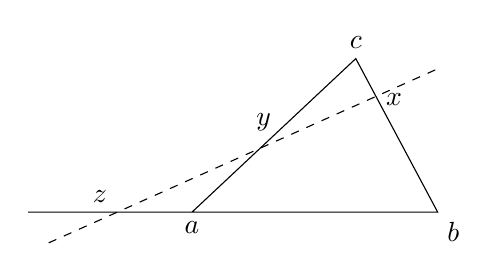
\begin{tikzpicture}[scale=1.3]
        \draw (-1,0)--(3,0)--(2.2, 1.5)--(0.6,0);
        \node[below] at (0.6, 0) {$a$};
        \node[below right] at (3,0) {$b$};
        \node[above] at (2.2, 1.5) {$c$};
        \draw[dashed] (-0.8,-0.3)--(3,1.4);
        \node[above] at (-0.3, 0) {$z$};
        \node[above] at (1.3, 0.7) {$y$};
        \node[right] at (2.4, 1.1) {$x$};
      \end{tikzpicture}\]
      Suppose that they divide these sides in the ratio 
      \[\lambda: 1, \mu: 1, \nu: 1\]
      respectively. Then, the points $x, y, z$ lie on the same line if and only if 
      \[\lambda \mu \nu = -1\]
    \end{corollary}
    \begin{proof}
    By the previous theorem, the points $x, y, z$ are linearly dependent (i.e. lies on a line) if and only if the matrix of barycentric coordinates of $x, y, z$ with respect to $a, b, c$, which is
    \begin{equation}
      \begin{pmatrix}
      0 & \frac{1}{\lambda + 1} & \frac{\lambda}{\lambda + 1} \\
      \frac{\mu}{\mu + 1} & 0 & \frac{1}{\mu + 1} \\
      \frac{1}{\nu + 1} & \frac{\nu}{\nu+1} & 0
      \end{pmatrix}
    \end{equation}
    has nonzero determinant. The determinant of the above matrix is $0$ if and only if $\lambda \mu \nu = -1$. 
    \end{proof}

    \begin{corollary}[Ceva's Theorem]
      In the triangle above, the lines $ax, by, cz$ intersect at one point if and only if 
      \begin{equation}
        \lambda \mu \nu = 1
      \end{equation}
    \end{corollary}
    \begin{proof}
      The proof can be done using barycentric coordinates. 
    \end{proof}

    \begin{theorem}
      A nonempty subset $P \subset S$ is a plane if and only if for any two distinct points $a, b \in P$, the line through $a$ and $b$ also lies in $P$. 
    \end{theorem}

    \begin{theorem}
      Given an inhomogeneous system of linear equations of form 
      \begin{equation}
        A x = b
      \end{equation}
      the set of solutions is an affine plane of dimension $n-r$, where $n$ is the number of variables and $r$ is the rank of the matrix $A$. More precisely, given that the plane is in the form $P = p_0 + U$, $p_0$ is one solution and $U$ is the set of vectors that satisfy the homogeneous system
      \begin{equation}
        Ax = 0
      \end{equation}
    \end{theorem}

    Let us observe the relative position of two planes. 

    \begin{theorem}
      Given two planes 
      \begin{align*}
        P_1 = p_1 + U_1, & P_2 = p_2 + U_2
      \end{align*}
      $P_1$ and $P_2$ intersect if and only if 
      \begin{equation}
        \overline{p_1 p_2} \subset U_1 + U_2
      \end{equation}
      where $U_1 + U_2$ is the set of all vectors of form $u_1 + u_2$, where $u_1 \in U_1, u_2 \in U_2$. 
    \end{theorem}

    Now, consider the class of functions on an affine space corresponding to the class of linear functions on a vector space. 

    \begin{definition}
      An \textit{affine-linear} function on an affine space $S$ is a function $f: S \longrightarrow \mathbb{F}$ such that
      \begin{equation}
        f(p + x) = f(p) + \alpha (x), \;\; p \in S , x \in V
      \end{equation}
      where $\alpha$, called the \textit{differential}, is a linear function on the vector space $V$. Let $o \in S$ be a fixed origin. By setting $p = o$, we can express an affine linear function in vectorized form as 
      \begin{equation}
        f(x) = \alpha (x) + b, \;\; b \in \mathbb{F}
      \end{equation}
      where $b = f(o)$. This implies the following coordinate form of $f$. 
      \begin{equation}
        f(x) = b + \sum_i a_i x_i
      \end{equation}
    \end{definition}

    A particular case of affine-linear functions are constant functions, where the defining characteristic is the zero differential. 

    \begin{proposition}
      Given that $\dim{S} = n$, affine-linear functions on $S$ form a $(n+1)$-dimensional subspace on the space of all linear functions on $S$. 
    \end{proposition}

    \begin{proposition}
      Barycentric coordinates are affine-linear functions. 
    \end{proposition}

    \begin{proposition}
      Let $f$ be an affine-linear function. Then
      \begin{equation}
        f \bigg( \sum_i \lambda_i p_i \bigg) = \sum_i \lambda_i f(p_i)
      \end{equation}
      for any barycentric linear combination $\sum_i \lambda_i p_i$ of points $p_1, ..., p_k$. 
    \end{proposition}

    \begin{definition}
      An affine space associated with a Euclidean vector space is called a \textit{Euclidean affine space}. The \textit{distance $\rho$} between two points in a Euclidean space is defined as
      \begin{equation}
        \rho(p, q) = ||\overline{pq}||
      \end{equation}
      This definition of $\rho$ satisfies the axioms of a metric space. 
    \end{definition}

  \subsection{Convex Sets}

    Let $S$ be an affine space over the field of real numbers and $V$, the associated vector space. 

    \begin{definition}
      The \textit{(closed) interval} connecting points $p, q \in S$ is the set
      \begin{equation}
        pq = \{\lambda p + (1-\lambda) q \;|\; 0 \leq \lambda \leq 1\}
      \end{equation}
      Geometrically, we can think of this as the straight line segment connecting point $p$ with point $q$. 
    \end{definition}

    \begin{definition}
      A set $M \subset S$ is \textit{convex} if for any two points $p, q \in S$, it contains the whole interval $p, q$. 
    \end{definition}

    Clearly, the intersection of convex sets is convex. However, the union of them is not. 

    \begin{definition}
      A \textit{convex linear combination} of points in $S$ is their barycentric linear combination with nonnegative coefficients. 
    \end{definition}

    It is clear to visualize the following proposition. 

    \begin{proposition}
      For any points $p_0, ..., p_k$ in a convex set $M \subset S$, the set $M$ also contains every convex linear combination 
      \begin{equation}
        p = \sum_i \lambda_i p_i
      \end{equation}
      Furthermore, for any set $M \subset S$, the set $\conv{M}$ of all convex linear combinations of points in $M$ is convex. 
    \end{proposition}

    \begin{definition}
      Given $M \subset S$, the set $\conv M$ is the smallest convex set containing $M$. It is called the \textit{convex hull} of $M$. 
    \end{definition}

    \begin{definition}
      The convex hull of a system of affinely independent points $p_0, p_1, ..., p_n$ in an $n$-dimensional affine space is called the \textit{$n$-dimensional simplex} with vertices $p_0, ..., p_n$. 
    \end{definition}

    It is clear that the interior points of a simplex is precisely the set of all points whose barycentric coordinates with respect to the vertices are all positive. 

    \begin{example}
      Here are common examples of simplices.
      \begin{enumerate}
        \item A $0$-dimensional simplex is a point. 
        \item A $1$-dimensional simplex is a closed line interval. 
        \item A $2$-dimensional simplex is a triangle. 
        \item A $3$-dimensional simplex is a tetrahedron. 
      \end{enumerate}
    \end{example}

    \begin{proposition}
      A convex set $M$ has interior points if and only if $\aff M = S$. 
    \end{proposition}

    \begin{definition}
      A convex set that has interior points is called a \textit{convex body}. Clearly, every convex body in $n$-dimensional affine space $S$ is $n$-dimensional. 
    \end{definition}

    The set of interior points of a convex body $M$, denoted $M^\circ$, is an open convex body. 

    \begin{definition}
      For any nonconstant affine-linear function $f$ on the set $S$, let
      \begin{align*}
        H_f \equiv \{p \in S \;|\; f(p) = 0\} \\
        H^+_f \equiv \{p \in S \;|\; f(p) \geq 0\} \\
        H^-_f \equiv \{p \in S \;|\; f(p) \leq 0\}
      \end{align*}
      The set $H_f$ is a hyperplane, and $H^+_f, H^-_f$ are called \textit{closed half spaces}. 
    \end{definition}

    \begin{definition}
      A hyperplane $H_f$ is a \textit{supporting hyperplane} of a closed convex body $M$ if $M \subset H^+_f$ and $H_f$ contains at least one (boundary) point of $M$. The half space $H^+_f$ is then called the \textit{supporting half-space} of $M$. 
    \end{definition}

    \begin{proposition}
      A hyperplane $H$ that passes through a boundary point of a closed convex body $M$, is supporting if and only if $H \cap M^\circ = \emptyset$. 
    \end{proposition}

    A key theorem of convex sets is the following separation theorem. 

    \begin{theorem}[Separation Theorem]
      For every boundary point of a closed convex body, there exists a supporting hyperplane passing through this point. 
    \end{theorem}

    This theorem leads to the following one. 

    \begin{theorem}
      Every closed convex set $M$ is an intersection of (perhaps infinitely many) half-spaces. 
    \end{theorem}

    \begin{definition}
      A \textit{polyhedron} is the intersection of a finite number of half-spaces. A convex polyhedron which is also a body is called a \textit{convex solid}. 
    \end{definition}

    \begin{example}
      A simplex with vertices $p_0, p_1, ..., p_n$ is a convex polyhedron since it is determined by linear inequalities $x_i \geq 0$ for $i = 0, 1, ..., n$, where $x_0, x_1, ..., x_n$ are barycentric coordiantes with respect to $p_0, p_1,..., p_n$. 
    \end{example}

    \begin{example}
      A convex polyhedron determined by linear inequalities $0 \leq x_i \leq 1$ for $i = 1, ..., n$, where $x_1,..., x_n$ are affine coordinates with respect ot some frame, is called an $n$-dimensional parallelopiped. 
    \end{example}

    \begin{definition}
      A point $p$ of a convex set $M$ is \textit{extreme} if it is not an interior point of any interval in $M$. 
    \end{definition}

    \begin{theorem}
      A bounded closed convex set $M$ is the convex hull of the set $E(M)$ of its extreme points. 
    \end{theorem}

    We can create a stronger statement with the following theorem. 

    \begin{theorem}[Minkowski-Weyl Theorem]
      The following properties of a bounded set $M \subset S$ is equivalent.
      \begin{enumerate}
        \item $M$ is a convex polyhedron. 
        \item $M$ is a convex hull of a finite number of points. 
      \end{enumerate}
    \end{theorem}

    \begin{definition}
      A \textit{face} of a convex polyhedron $M$ is a nonempty intersection of $M$ with some of its supporting hyperplanes. Given that $\dim \aff M = n$, 
      \begin{enumerate}
        \item A $0$-dimensional face is called a \textit{vertex}. 
        \item A $1$-dimensional face an \textit{edge}. 
        \item ...
        \item An $(n-1)$-dimensional face a \textit{hyperface}. 
      \end{enumerate}
    \end{definition}

    Therefore, if a convex polyhedron is determined by a system of linear inequalities, we can obtain its faces by replacing some of these inequalities with equalities (in such a way that we do not get the empty set). 

    The following theorem demonstrates that in order to find its faces, it suffices to consider only the hyperplanes $H_{f_1}, ..., H_{f_m}$. 

    \begin{theorem}
      Every face $\Gamma$ of the polyhedron $M$ is of the form
      \begin{equation}
        \Gamma = M \cap \bigg( \bigcap_{j \in J} H_{f_j} \bigg)
      \end{equation}
      where $J = \{1, 2, ..., m\}$
    \end{theorem}

    \begin{proposition}
      The extreme points of a convex polyhedron $M$ are exactly its vertices. 
    \end{proposition}

    The following theorem is used often in linear programming and in optimization. 

    \begin{theorem}
      The maximum of an affine-linear function on a bounded convex polyhedron $M$ is attained at a vertex. 
    \end{theorem}

  \subsection{Affine Transformations and Motions}

    Let $S$ and $S^\prime$ be affine spaces associated with vector spaces $V$ and $V^\prime$, respectively, over the same field $\mathbb{F}$. 

    \begin{definition}
      An \textit{affine map} from the space $S$ to the space $S^\prime$ is a map $f: S \longrightarrow S^\prime$ such that
      \begin{equation}
        f(p+x) = f(p) + \varphi(x), \;\; p \in S, x \in V
      \end{equation}
      for some linear map $\varphi: V \longrightarrow V^\prime$. It follows that
      \begin{equation}
        \varphi(\overline{pq}) = \overline{f(p) f(q)}, \;\; p, q \in S
      \end{equation}
      Thus, $f$ determines the linear map $\varphi$ uniquely. Similarly, $\varphi$ is called the \textit{differential} of $f$, denoted $df$. 
    \end{definition}

    \begin{proposition}
      Let $f: S \longrightarrow S^\prime$ and $g: S^\prime \longrightarrow S^{\prime \prime}$ be two affine maps. Then the map
      \begin{equation}
        g \circ f : S \longrightarrow S^{\prime\prime}
      \end{equation}
      is also affine. Also
      \begin{equation}
        d(g \circ f) = dg \cdot df
      \end{equation}
      where $dg$ and $df$ are the differentials of $g$ and $f$, respectively. 
    \end{proposition}

    For $\mathbb{F} = \mathbb{R}$, the differential of an affine map is a particular case of a differential of a smooth map in analysis. That is, the differential is the linear approximation of the function $f$. 

    \begin{proposition}
      An affine map is bijective if and only if its differential is bijective. 
    \end{proposition}

    \begin{definition}
      Similar to linear transformations between vector spaces, bijective affine transformations are called \textit{isomorphisms} of affine spaces. Affine spaces are \textit{isomorphic} if there exists an isomorphism between them. 
    \end{definition}

    \begin{corollary}
      Finite-dimensional affine spaces over the same field are isomorphic if and only if they have the same dimension. 
    \end{corollary}

    \begin{definition}
      An affine map from an affine space $S$ to itself is called an \textit{affine transformation}. Bijective affine transformations form a group called the \textit{affine group of $S$}, denoted $\GA(S)$. 
    \end{definition}

    It follows that given affine space $S$ with associated vector space $V$, the projection map
    \begin{equation}
      d: \GA(S) \longrightarrow \GL(V)
    \end{equation}
    is a group homomorphism. It's kernel is the group of parallel translations, called Tran$(S)$. 
    \begin{equation}
      t_a : p \mapsto p + a, \;\; a \in V
    \end{equation}

    \begin{proposition}
      For any $f \in \GA(S)$ and $a \in V$, 
      \begin{equation}
        f t_a f^{-1} = t_{df(a)}
      \end{equation}
    \end{proposition}

    \begin{definition}
      A \textit{homothety} with the center $o$ and coefficient $\lambda$ is an affine transformation defined as
      \begin{equation}
        f( o + x ) \equiv o + \lambda x
      \end{equation}
      In its vectorized form, it is expressed
      \begin{equation}
        f(x) = \lambda x + b, \;\; b \in V
      \end{equation}
      A homothety with coefficient $-1$ is called a \textit{central symmetry}. 
    \end{definition}

    The group of affine transformations determines the \textit{affine geometry} of the space. The following theorem shows that all simplices are equal in affine geometry. 

    \begin{theorem}
      Let $\{p_0, ..., p_n\}$ and $\{q_0, ..., q_n\}$ be two systems of affinely independent points in an $n$-dimensional affine space $S$. Then there exists a unique affine transformation $f$ that maps $p_i$ to $q_i$ for $i = 0, 1, ..., n$. 
    \end{theorem}
    \begin{proof}
      It is easy to see once we realize that there exists a unique linear map $\varphi$ of the space $V$ that maps the basis $\{\overline{p_0 p_1}, ..., \overline{p_0 p_n}\}$ to the basis $\{\overline{q_0 q_1}, ..., \overline{q_0 q_n}\}$. If we vectorize $S$ by taking $p_0$ as the origin, the affine transformation in question has the form 
      \begin{equation}
        f(x) = \varphi(x) + \overline{p_0 q_0}
      \end{equation}
    \end{proof}

    \begin{corollary}
      In real affine geometry all parallelopipeds are equal. 
    \end{corollary}

    \begin{definition}
      A \textit{motion} of the space $S$ is an affine transformation of $S$ whose differential is an orthogonal operator (i.e. an origin preserving isometry). Every motion is bijective. 
    \end{definition}

    Motions of a Euclidean space $S$ form a group denoted Isom$\,S$. A motion is called \textit{proper (orientation preserving)} if its differential belongs to SO$(V)$ and improper otherwise. 

    \begin{lemma}
      The group Isom$\,S$ is generated by reflections through hyperplanes. 
    \end{lemma}

    \begin{definition}
      Let $M$ be a solid convex polyhedron in an $n$-dimensional Euclidean space. A \textit{flag of $M$} is a collection of its faces $\{F_0, F_1, ..., F_{n-1}\}$ where $\dim{F_k} = k$ and $F_0 \subset F_1 \subset ... \subset F_{n-1}$. 
    \end{definition}

    \begin{definition}
      A convex polyhedron $M$ is \textit{regular} if for any two of its flags, there exists a motion $f \in$ Sym$\,M$ mapping the first to the second, where 
      \begin{equation}
        \text{Sym}\,M \equiv \{f \in \text{Isom}\,S \;|\; f(M) = M \}
      \end{equation}
    \end{definition}

    Two dimensional regular polyhedra are the ordinary \textit{regular polygons}. Their symmetry groups are known as the dihedral groups.

    Three dimensional regular polyhedra are \textit{Platonic solids}, which are the regular tetrahedron, cube, octahedron, dodecahedron, and icosahedron. 

    \begin{definition}
      A real vector space $V$ with a fixed symmetric bilinear function $\alpha$ of signature $(k, l)$, where $k, l > 0$ and $\dim{V} = k+l$, is called the \textit{pseudo-Euclidean vector space} of signature $(k, l)$. The group of $\alpha$-preserving linear transformations of $V$ is called the \textit{pseudo-orthogonal group} and is denoted O$(V, \alpha)$. In an orthonormal basis, the corresponding matrix group is denoted $O{k,l}$. 
    \end{definition}

  \subsection{Quadrics}

    Planes are the simplest objects of affine and Euclidean geometry, which are determined by systems of linear equations. The second simplest are quadratic functions. These types of objects are studied futher in algebraic geometry. 

    \begin{definition}
      An \textit{affine-quadratic function} on an affine space $S$ is a function $Q: S \longrightarrow \mathbb{F}$ such that its vectorized form is
      \begin{equation}
        Q(x) = q(x) + l(x) + c
      \end{equation}
      for a quadratic function $q$, linear function $l$, and constant $c$. 
    \end{definition}

  \subsection{Projective Spaces}

    \begin{definition}
      An $n$-dimensional \textit{projective space $PV$} over a field $\mathbb{F}$ is the set of one-dimensional subspaces of an $(n+1)$-dimensional vector space $V$ over $\mathbb{F}$. For every $(k+1)$-dimensional subspace $U \subset V$, the subset $PU \subset PV$ is called a $k$-dimensional \textit{plane} of the space $PV$. 
      \begin{enumerate}
        \item $0$-dimensional planes are the points of $PV$. 
        \item $1$-dimensional planes are called \textit{lines}
        \item ...
        \item $(n-1)$-dimensional planes are called \textit{hyperplanes}
      \end{enumerate}
    \end{definition}

    \begin{definition}
      $\mathbb{RP}^1$ is called the real projective line, which is topologically equivalent to a circle. 
    \end{definition}

    \begin{example}
      The real projective space of $\mathbb{R}^2$ is the set of all lines that pass through the origin. It is denoted $\mathbb{R P}^2$ and called the \textit{real projective plane}. 
    \end{example}

    \begin{example}
      $\mathbb{RP}^3$ is diffeomorphic to SO$(3)$. 
    \end{example}

    \begin{example}
      The space $\mathbb{RP}^n$ is formed by taking the quotient of $\mathbb{R}^{n+1} \setminus \{0\}$ under the equivalence relation 
      \begin{equation}
        x \sim \lambda x \text{ for all real numbers } \lambda \neq 0
      \end{equation}
      The set of these equivalence classes is isomorphic to $\mathbb{RP}^n$. 
    \end{example}

\section{Tensor Algebras}

  Remember that an algebra is (loosely) a vector space $V$ with a multiplication operation
  \begin{equation}
    \times: V \times V \longrightarrow V
  \end{equation}

  \begin{definition}
    The \textit{tensor algebra} of vector space $V$ over field $\mathbb{F}$ is 
    \begin{align*}
      T(V) \equiv \bigoplus_{n = 0}^{\infty} V^{\otimes n} & = V^{\otimes 0} \oplus V^{\otimes 1} \oplus V^{\otimes 2} \oplus V^{\otimes 3} \oplus ... \\
      & = \mathbb{F} \oplus V \oplus V^{\otimes 2} \oplus V^{\otimes 3} \oplus V^{\otimes 4} \oplus ...
    \end{align*}
    with elements being infinite-tuples
    \begin{equation}
      (a, B^\mu, C^{\nu \gamma}, D^{\alpha \beta \epsilon}, ...)
    \end{equation}
    The addition operation is defined component-wise, and the multiplication operation is the tensor product 
    \begin{equation}
      \otimes: T(V) \times T(V) \longrightarrow T(V)
    \end{equation}
    and the identity element is
    \begin{equation}
      I = (1, 0, 0, ...)
    \end{equation}
    Linearity can be easily shown. 
  \end{definition}

  The tensor algebra is often used to "add" differently ranked tensors together. But in order to do this rigorously, we must define the canonical injections
  \begin{equation}
    i_j: V^{\otimes j} \longrightarrow T(V), \; i_j (T^{\kappa_1, ..., \kappa j}) = (0, ...,0, T^{\kappa_1, ..., \kappa j}, 0, ..., 0) 
  \end{equation}
  shown in the diagram
  \[\begin{tikzcd}
      & & T(V) & & \\
      \mathbb{F} \arrow{urr}{i_0} & V \arrow{ur}{i_1} & V^{\otimes 2} \arrow{u}{i_2} & V^{\otimes 3} \arrow{ul}{i_3} & ... \arrow{ull}
  \end{tikzcd}\]
  Therefore, with these $i_j$'s, we can implicitly define the addition of arbitrary tensors $A \in V^{\otimes n}$ and $B \in V^{\otimes m}$ as 
  \begin{equation}
    A + B \equiv i_n (A) + i_m (B) \in T(V)
  \end{equation}
  along with multiplication of tensors as
  \begin{equation}
    A \otimes B \equiv i_n(A) \otimes i_m(B) \equiv i_{n+m} (A \otimes B)
  \end{equation}
  We can also redefine the tensor product operation between two spaces to be an operation within $T(V)$ itself. 
  \begin{equation}
    i_i(V^{\otimes i}) \otimes i_j( V^{\otimes j}) = i_{i+j} (V^{\otimes (i+j)})
  \end{equation}
  We can now proceed to define Exterior and Symmetric algebras as quotient algebras. 

  \begin{definition}
    The \textit{exterior algebra} $\Lambda(V)$ of a vector space $V$ over field $\mathbb{F}$ is the quotient algebra of the tensor algebra $T(V)$
    \begin{equation}
      \Lambda(V) \equiv \frac{T(V)}{I}
    \end{equation}
    where $I$ is the two-sided ideal generated by all elements of the form $x \otimes x$ for $x \in V$ (i.e. all tensors that can be expressed as the tensor product of a vector in V by itself). 

    The \textit{exterior product} $\wedge$ of two elements of $\Lambda(V)$ is the product induced by the tensor product $\otimes$ of $T(V)$. That is, if 
    \begin{equation}
      \pi: T(V) \longrightarrow \Lambda(V)
    \end{equation}
    is the canonical projection/surjection and $a, b \in \Lambda(V)$ ,then there are $\alpha, \beta \in T(V)$ such that $a = \pi(\alpha), b = \pi(\beta)$, and 
    \begin{equation}
      a \wedge b = \pi(\alpha \otimes \beta)
    \end{equation}
    We can define this quotient space with the equivalence class
    \begin{equation}
      x \otimes y = - y \otimes x \pmod{I}
    \end{equation}
  \end{definition}

  \begin{definition}
    The \textit{symmetric algebra} Sym$(V)$ of a vector space $V$ over a field $\mathbb{F}$ is the quotient algebra of the tensor algebra $T(V)$ 
    \begin{equation}
      \Lambda(V) \equiv \frac{T(V)}{J}
    \end{equation}
    where $J$ is the two-sided ideal generated by all elements in the form 
    \begin{equation}
      v \otimes w - w \otimes v
    \end{equation}
    (i.e. commutators of all possible pairs of vectors). 
  \end{definition}

\section{Representation Theory}

  We will assume that $V$ is a finite-dimensional vector space over field $\mathbb{C}$. 

  \begin{definition}
    The \textit{general linear group} of vector space $V$, denoted $\GL(V)$, is the group of all automorphisms of $V$ to itself. The \textit{special linear group} of vector space $V$, denoted $\SL(V)$ is the subgroup of automorphisms of $V$ with determinant $1$. 
  \end{definition}

  When studying an abstract set, it is often useful to consider the set of all maps from this abstract set to a well known set (e.g. $\GL(V)$). 

  \begin{definition}
    A \textit{representation} of an (algebraic) group $\mathcal{G}$ is a homomorphism 
    \begin{equation}
      \rho: G \longrightarrow \GL(V)
    \end{equation}
    for some vector space $V$. That is, given an element $g \in \mathcal{G}$, $\rho(g) \in \GL (V)$, meaning that $\rho(g)(v) \in V$. Additionally, since it is a homomorphism, the algebraic structure is preserved. 
    \begin{equation}
      \rho(g_1 \cdot g_2) = \rho(g_1) \cdot \rho(g_2)
    \end{equation}
    where $\cdot$ on the left hand side is the abstract group multiplication while the $\cdot$ on the right hand side is matrix multiplication. To shorten the notation, we will denote 
    \begin{equation}
      g v = \rho(g) v, \; v \in V
    \end{equation}
    Since $\rho$ is a group morphism, we have 
    \begin{equation}
      g_2 (g_1 v) = (g_2 g_1) v \; \iff \rho(g_2) \big( \rho(g_1) (v) \big) = \big( \rho(g_2) \rho(g_1) \big) (v)
    \end{equation}
    Additionally, since $g$ (that is, $\rho(g)$) is a linear map, 
    \begin{equation}
      g(\lambda_1 v_1 + \lambda_2 v_2) = \lambda_1 g v_1 + \lambda_2 g v_2
    \end{equation}
    Usually, we refer to the map as the representation, but if the map is well-understood, we just call the vector space $V$ the representation and say that the group acts on this vector space. 
  \end{definition}

  \begin{example}
    The group $\GL(2, \mathbb{C})$ can be represented a by the vector space $\mathbb{C}^2$, or explicitly, by the group of $2 \times 2$ matrices over $\mathbb{C}$ with nonzero determinant.
    \begin{equation}
      \GL(2, \mathbb{C}) \xmapsto{id} \text{Mat}(2, \mathbb{C})
    \end{equation}
    This is a trivial representation. 
  \end{example}

  We now show a nontrivial representation of $\GL(2, \mathbb{C})$. 

  \begin{example}
    We take Sym$^2 \mathbb{C}^2$, the second symmetric power of $\mathbb{C}^2$. Note that given a basis $x_1, x_2 \in \mathbb{C}^2$, the set
    \begin{equation}
      \{x_1 \odot x_1, x_1 \odot x_2, x_2 \odot x_2\}
    \end{equation}
    forms a basis of Sym$^2 \mathbb{C}^2 \implies \dim\,$Sym$^2 \mathbb{C}^2 = 3$. So, we want to represent $\GL(2, \mathbb{C})$ by associating its element with elements of $\GL(Sym^2 \mathbb{C}^2)$. More concretely, we are choosing to represent a $2 \times 2$ matrix over $\mathbb{C}$ with a $3 \times 3$ matrix group (since $\GL(Sym^2 \mathbb{C}^2) \simeq \GL(3, \mathbb{C})$. Clearly,
    \begin{align*}
      & \rho(g) (x_1 \odot x_1) = g(x_1) \odot g(x_1) \in Sym^2 \mathbb{C}^2 \\
      & \rho(g) (x_1 \odot x_2) = g(x_1) \odot g(x_2) \\
      & \rho(g) (x_2 \odot x_2) = g(x_2) \odot g(x_2)
    \end{align*}
    To present this in matrix form, let us have an element in $\GL (2, \mathbb{C})$
    \begin{equation}
      \mathcal{A} \equiv \begin{pmatrix}
      a & b \\
      c & d
      \end{pmatrix}
    \end{equation}
    We evaluate the corresponding representation in $\GL( Sym^2 \mathbb{C}^2)$. Using the identities above, we have 
    \begin{align*}
      \rho(g) (x_1 \odot x_1) & = g(x_1) \odot g(x_1) \\
      & = (a x_1 + c x_2) \odot (a x_1 + c x_2) \\
      & = a^2 x_1 \odot x_1 + 2ac x_1 \odot x_2 + c^2 x_2 \odot x_2 \\
      \rho(g) (x_1 \odot x_2) & = g(x_1) \odot g(x_2) \\
      & = (a x_1 + c x_2) \odot (b x_1 + d x_2) \\
      & = ab x_1 \odot x_1 + (ad + bc) x_1 \odot x_2 + cd x_2 \odot x_2 \\
      \rho(g) (x_2 \odot x_2) & = g(x_2) \odot g(x_2) \\
      & = (b x_1 + d x_2) \odot (b x_1 + d x_2) \\
      & = b^2 x_1 \odot x_1 + 2bd x_1 \odot x_2 + d^2 x_2 \odot x_2
    \end{align*}
    And this completely determines the matrix. So, 
    \begin{equation}
      \rho \begin{pmatrix}
      a&b\\c&d
      \end{pmatrix} = \begin{pmatrix}
      a^2&ab&b^2\\2ac&ad+bc&2bd\\c^2&cd&d^2
      \end{pmatrix}
    \end{equation}
    is the $3 \times 3$ representation of $\mathcal{A}$ in $\GL(Sym^2 \mathbb{C}^2)$. 
  \end{example}

  We continue to define maps between two representations of $\mathcal{G}$. 

  \begin{definition}
    A \textit{morphism} between 2 representations 
    \begin{align*}
      & \rho_1: \mathcal{G} \longrightarrow \GL(V_1) \\
      & \rho_2: \mathcal{G} \longrightarrow \GL(V_2) 
    \end{align*}
    of some group but not necessarily the same vector space is a linear map $f: V_1 \longrightarrow V_2$ that is \textit{compatible} with the group action. That is, $f$ satisfies the property that for all $g \in \mathcal{G}$
    \begin{equation}
      f \circ g = g \circ f
    \end{equation}
    Again, we use the shorthand notation that $g = \rho(g)$, meaning that the statement above really translates to $ f \circ \rho(g) = \rho(g) \circ f$. This is equivalent to saying that the following diagram commutes. 
    \[\begin{tikzcd}
    V_1 \arrow{r}{\rho_1(g)} \arrow{d}{f} & V_1 \arrow{d}{f} \\
    V_2 \arrow{r}{\rho_2 (g)} & V_2
    \end{tikzcd}\]
  \end{definition}

  \begin{definition}
    Let $V$ be a representation of $\mathcal{G}$. A \textit{subrepresentation} is a subspace $W \subset V$ such that for all $g \in \mathcal{G}$ and for all $w \in W$, 
    \begin{equation}
      \rho(g)(w) \in W
    \end{equation}
  \end{definition}

  \begin{example}
    $V$ and $\{0\}$ are always subrepresentations of $V$. 
  \end{example}

  We now introduce the "building blocks" of all representations. 
  \begin{definition}
    A representation $W$ is \textit{irreducible representation} if $\{0\}$ and $W$ are the only subrepresentations of $W$. 
  \end{definition}

  \begin{lemma}[Schur's Lemma]
    Let $V_1, V_2$ be irreducible representations and let $f: V_1 \longrightarrow V_2$ be a morphism (of representations). Then, either
    \begin{enumerate}
      \item $f$ is an isomorphism. 
      \item $f = 0$
    \end{enumerate}
    Furthermore, any 2 isomorphisms differ by a constant. That is, 
    \begin{equation}
      f_1 = \lambda f_2
    \end{equation}
  \end{lemma}
  \begin{proof}
    $\ker{f}$ is clearly a vector space. Furthermore, it is a subrepresentation (since it is a subspace of $V_1$) $\implies \ker{f} = V$ or $\ker{f} = 0$. If $\ker{f} = V$, then $f = 0$ and the theorem is satisfied. If $\ker{f} = 0$, then $f$ is injective, and $\im{f}$ is a subrepresentation of $V_2 \implies \im{f} = 0$ or $\im{f} = V_2$. But $\im{f} \neq 0$ since $f$ is injective, so $\im{f} = V_2 \implies f$ is surjective $\implies f$ is bijective, that is, $f$ is an isomorphism of vector spaces. So, the inverse $f^{-1}$ exists, and this map $f^{-1}$ satisfies
    \begin{equation}
      f^{-1} \circ \rho_2(g) = \rho_1 (g) \circ f^{-1}
    \end{equation}
    To prove the second part, without loss of generality, assume that the first isomorphism is the identity mapping. That is, 
    \begin{equation}
      f_1 = id
    \end{equation}
    Since we are working over the field $\mathbb{C}$, we can find an eigenvector of $f_2$. That is, there exists a $v \in V_1$ such that 
    \begin{equation}
      f_2 (v) = \lambda v
    \end{equation}
    Now, we define the map
    \begin{equation}
      f: V_1 \longrightarrow V_2, \; f \equiv f_2 - \lambda f_1
    \end{equation}
    Clearly, $\ker{f} \neq 0$, since $v \in \ker{f}$. That is, we have a map $f$ between 2 irreducible representations that has a nontrivial kernel. This means that $f = 0 \implies f_2 = \lambda f_1$.  
  \end{proof}

  \begin{theorem}[Mache's Theorem]
    Let $V$ be finite dimensional, with $\mathcal{G}$ a finite group. Then, $V$ can be decomposed as 
    \begin{equation}
      V = \bigoplus_{i} V_i
    \end{equation}
    where each $V_i$ is an irreducible representation of $\mathcal{G}$. 
  \end{theorem}
  \begin{proof}
    By induction on dimension, it suffices to prove that if $W$ is a subrepresentation of $V$, then there exists a subrepresentation $W^\prime \subset V$ such that $W \oplus W^\prime = V$. So, if $V$ isn't an irreducible representation, it can always be decomposed into smaller subrepresentations $W$ and $W^\prime$ that direct sum to $V$. Now, we define the canonical (linear) projection 
    \begin{equation}
      \pi: V \longrightarrow W
    \end{equation}
    Then, we define the new map 
    \begin{equation}
      \Tilde{\pi}: V \longrightarrow W, \; \Tilde{\pi}(v) \equiv \frac{1}{|\mathcal{G}|} \sum_{g \in \mathcal{G}} \rho(g)\big|_W \circ \pi \circ \rho(g)^{-1}
    \end{equation}
    This "averaging" of the group elements are done so that this mapping is a map of representations. This implies that 
    \begin{equation}
      V = W \oplus \ker{\Tilde{\pi}}
    \end{equation}
    meaning that $V$ can indeed be decomposed into direct sums of subrepresentations. 
  \end{proof}

\section{Lie Groups and Lie Algebras}

    \begin{definition}
      A \textit{Lie group} is a group $\mathcal{G}$ that is also a finite-dimensional smooth manifold, in which the group operations of multiplication and inversion are smooth maps. Smoothness of the group multiplication
      \begin{equation}
        \mu: \mathcal{G} \times \mathcal{G} \longrightarrow \mathcal{G}, \; \mu(x, y) = x y
      \end{equation}
      means that $\mu$ is a smooth mapping of the product manifold $\mathcal{G} \times \mathcal{G}$ into $\mathcal{G}$. These two requirements can be combined to the single requirement that tahe mapping 
      \begin{equation}
        (x, y) \mapsto x^{-1} y
      \end{equation}
      be a smooth mapping of the product manifold into $\mathcal{G}$. 
    \end{definition}

    \begin{definition}
      A \textit{Lie Algebra} is a vector space $\mathfrak{g}$ with an operation called the \textit{Lie Bracket} 
      \begin{equation}
        [\cdot, \cdot]: \mathfrak{g} \times \mathfrak{g} \longrightarrow \mathfrak{g}
      \end{equation}
      Satisfying
      \begin{enumerate}
        \item Bilinearity: $[ax + by, z] = a[x,z] + b[y,z], \; [z, ax + by] = a[z, x] + b[z,y]$
        \item Anticommutativity: $[x,y] = -[y,x]$
        \item Jacobi Identity: $[x,[y,z]] + [y,[z,x]] + [z,[x,y]] = 0$
      \end{enumerate}
      Clearly, this implies that $\mathfrak{g}$ is a nonassociative algebra. Note that a Lie Algebra does not necessarily need to be an algebra in the sense that there needs to be multiplication operation that is closed in $\mathfrak{g}$. 
    \end{definition}

    \begin{example}
      A common example of a Lie Braket in the algebra of matrices is defined
      \begin{equation}
        [A, B] \equiv AB - BA
      \end{equation}
      called the \textit{commutator}. Note that in this case, the definition of the Lie bracket is dependent on the definition of the matrix multiplication. Without defining the multiplication operation, we wouldn't know what $AB$ or $BA$ means. Therefore, we see that the Lie algebra of $n \times n$ matrices has three operations: matrix addition, matrix multiplication, and the commutator (along with scalar multiplication). But in general, it is not necessary to have that multiplication operation for abstract Lie algebras. $\mathfrak{g}$ just needs to be a vector space with the bracket.  
    \end{example}

    \begin{example}
      The set of all symmetric matrices is a vector space, but it is \textit{not} a Lie algebra since the commutator $[A,B]$ is not symmetric unless $A B = B A$. 
    \end{example}

    We will first talk about groups of matrices as a more concerete example before we get into abstract Lie groups. Recall that the matrix exponential map is defined
    \begin{equation}
      exp: \text{Mat}(n, \mathbb{C}) \longrightarrow \text{mat}(n, \mathbb{C}), \; exp(A) = e^A = \sum_{p \geq 0} \frac{A^p}{p!}
    \end{equation}
    Note that this value is always well defined. This lets us define
    \begin{equation}
      exp(t A) \equiv e^{t A} \equiv I + tA + \frac{1}{2} t^2 A^2 + \frac{1}{3!} t^3 A^3 + ... 
    \end{equation}
    where if $t$ is small, we can expect a convergence. Note that exp maps addition to multiplication. That is, we can interpret it as a homomorphism from 
    \begin{equation}
      exp: \mathfrak{g} \longrightarrow \mathcal{G}
    \end{equation}
    where $\mathfrak{g}$ is the Lie algebra and $\mathcal{G}$ is the Lie group (which we will treat just as a matrix group). To find the inverse of the exponential map, we can take the derivative of $e^{tA}$ at $t=0$. That is, 
    \begin{align*}
      \bigg(\frac{d}{d t} e^{tA} \bigg) \bigg|_{t=0} & = \bigg(\sum_{k=0}^\infty \frac{1}{k!} t^k A^{k+1} \bigg) \bigg|_{t=0} = A
    \end{align*}
    So, the mapping
    \begin{equation}
      \frac{d}{dt} \bigg|_{t=0}: \mathcal{G} \longrightarrow \mathfrak{g}
    \end{equation}
    maps the Lie group back to the algebra. We can interpret this above mapping by visualizing the Lie Algebra as a tangent (vector) space of the abstract Lie group $\mathcal{G}$ at the identity element of the Lie group. The visualization below isn't the most abstract one, but it may help:
    \begin{center}
      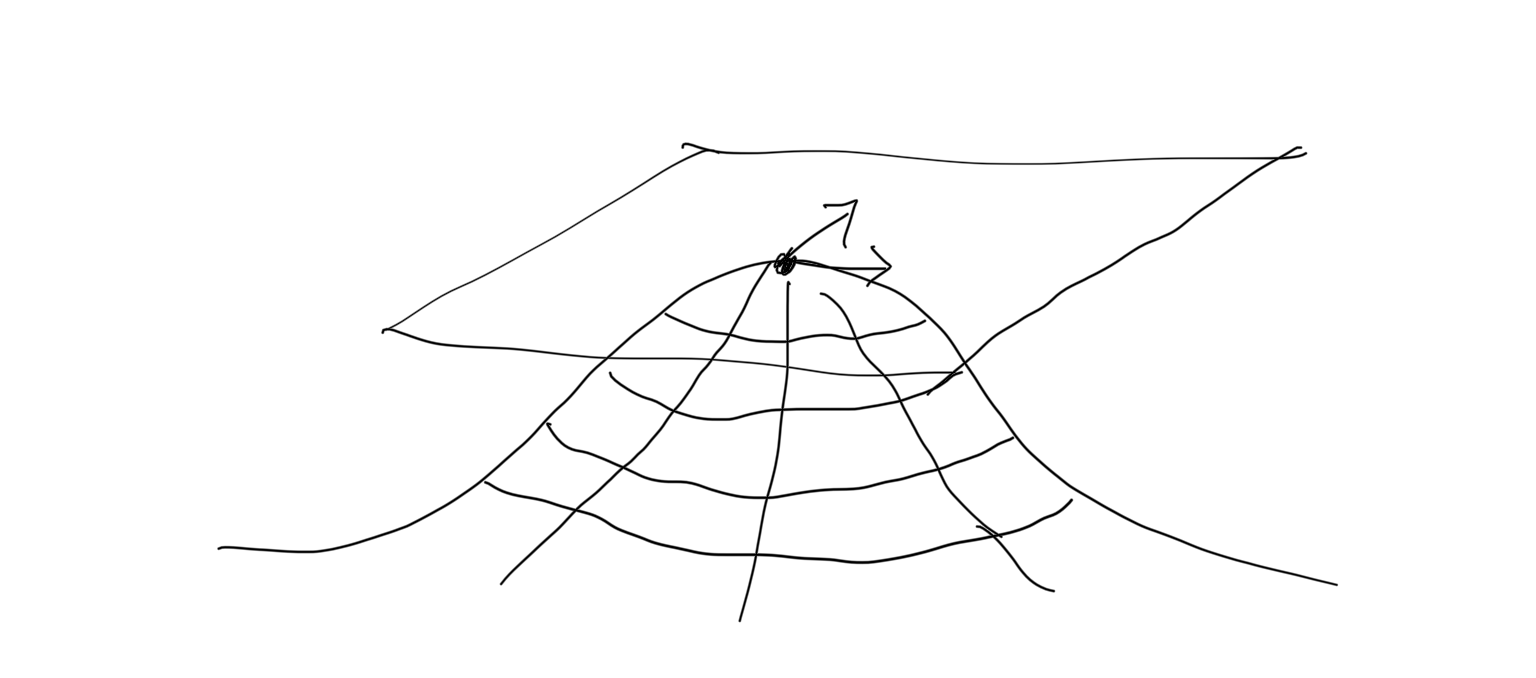
\includegraphics[scale=0.2]{img/Lie_Algebra_Tangent_Space.PNG}
    \end{center}
    For example, say that the Lie group $\mathcal{G}$ is a unit circle in $\mathbb{C}$, then the Lie algebra of $\mathcal{G}$ is the tangent space at the identity $1$, which can be identified as the imaginary line in the complex plane $\{i t \; | \; t \in \mathbb{R}\}$, with 
    \begin{equation}
      i t \mapsto exp(it) \equiv e^{it} \equiv \cos{t} + i \sin{t}
    \end{equation}

    \begin{center}
      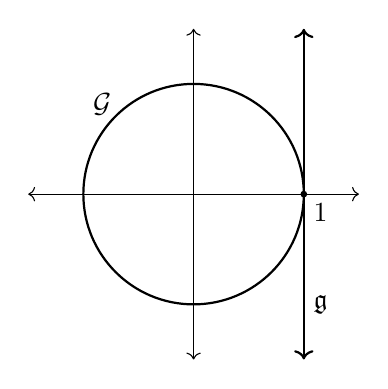
\begin{tikzpicture}[scale=0.7]
        \draw[thick] (0,0) circle (2);
        \node[below right] at (-2,2) {$\mathcal{G}$};
        \draw[<->] (-3,0)--(3,0);
        \draw[<->] (0,-3)--(0,3);
        \draw[fill] (2,0) circle (0.05);
        \node[below right] at (2,0) {$1$};
        \draw[thick, <->] (2,-3)--(2,3);
        \node[right] at (2,-2) {$\mathfrak{g}$};
      \end{tikzpicture}
    \end{center}
    So, analyzing the Lie group by looking at its Lie algebra turns a nonlinear problem to a linear one; this is called a \textit{linearization} of the Lie group. The existence of this exponential map is one of the primary reasons that Lie algebras are useful for studying Lie groups. 

    \begin{example}
      The exponential map 
      \begin{equation}
        exp: \mathbb{R} \longrightarrow \mathbb{R}^+, \; x \mapsto e^x
      \end{equation}
      is a group homomorphism that maps $(\mathbb{R}, +)$ to $(\mathbb{R}^+, \times)$. This means that $\mathbb{R}$ is the Lie algebra of the Lie group $\mathbb{R}^+$. 
    \end{example}

    \begin{theorem}
      If $A$ and $B$ are commuting square matrices, then 
      \begin{equation}
        e^{A + B} = e^A \, e^B
      \end{equation}
      In general, the solution $C$ to the equation
      \begin{equation}
        e^{A} \, e^B = e^C
      \end{equation}
      is given by the \textit{Baker-Campbell-Hausdorff formula}, defined
      \begin{equation}
        C = A + B + \frac{1}{2}[A,B] + \frac{1}{12} [A,[A,B]] - \frac{1}{12} [B,[A,B]] + ...
      \end{equation}
      consisting of terms involving higher commutators of $A$ and $B$. The full series is much too complicated to write, so we ask the reader to be satisfied with what is shown. 
    \end{theorem}

    The BCH formula is messy, but it allows us to compute products in the Lie Group as long as we known the commutators in the Lie Algebra. 

    Therefore, we can describe the process of constructing a Lie group from a Lie Algebra (which a vector space) as such. We take a vector space $V$ and endow it the additional bracket operation. We denote this as
    \begin{equation}
      \mathfrak{g} \equiv (V, [\cdot, \cdot])
    \end{equation}
    Then, we take every element of $\mathfrak{g}$ and apply the exponential map to them to get an another set $\mathcal{G}$. We then endow a group structure on $\mathcal{G}$ by defining the multiplication as 
    \begin{equation}
      \cdot: \mathcal{G} \times \mathcal{G} \longrightarrow \mathcal{G}, \; e^A \cdot e^B = e^{A * B}
    \end{equation}
    where $A*B$ is defined by the BCH formula up to a certain $k$th order. Since the $*$ operation is completely defined by the bracket in the Lie algebra, it tells us how to multiply in the Lie group. This process can be made more abstractly, depending on what $A, B$ and $[\cdot,\cdot]$ is, beyond matrices. 

  \subsection{Lie Algebras of Classical Lie Groups}

    \begin{definition}
      The \textit{general linear group} of vector space $V$ is the group of all automorphisms of $V$, denoted $\GL(V)$. Additionally, $\GL(n, \mathbb{R})$ is the group of real $n \times n$ matrices with nonzero determinant, and $\SL(n, \mathbb{R})$ is the group of real $n \times n$ matrices with determinant $= 1$.
    \end{definition}

    \subsubsection[Lie Algebras of SL(2, R) and SL(2, C)]{Lie Algebras of $\SL(2, \mathbb{R})$ and $\SL(2, \mathbb{C})$}

      Given the group $\SL(2, \mathbb{R})$, there must be a corresponding Lie algebra of matrices such that $g = e^A \in \SL(2, \mathbb{R})$. We attempt to find this Lie algebra. Let $g \in \SL(2, \mathbb{R})$, with $g = e^A$. So, if $\det{g} = 1$, what is the corresponding restriction on $A$ in the algebra? We use the following proposition. 

      \begin{proposition}
        \begin{equation}
          \det{(e^A)} = e^{\Tr{(A)}}
        \end{equation}
      \end{proposition}
      \begin{proof}
        Put $A$ in Jordan Normal Form: $A = S^{-1} J S \implies A^n = S^{-1} J^n S \implies exp(A) = S^{-1} exp(A) S \implies \det{(exp(A))} = \det{e^J}$. But since $J$ is upper trianglar, $J^n$ is upper triangular $\implies e^J$ is upper triangular, which implies that 
        \begin{equation}
          \det{e^J} = \prod_i e^{\lambda_i} = e^{\Tr{(J)}} = e^{\Tr{(A)}}
        \end{equation}
        since trace is invariant under a change of basis. 
      \end{proof}

      So, $\det{(e^A)} = 1 \implies \Tr{(A)} = 2 \pi i n$ for $n \in \mathbb{Z}$. Since we want to component connected to the identity, we choose $n=0$ meaning that $\Tr{(A)} = 0$. And we are done. That is, the Lie algebra of $\SL(2, \mathbb{R})$ consists of traceless $2 \times 2$ matrices, denoted $\mathfrak{sl}_2 \mathbb{R}$. $\mathfrak{sl}_2 \mathbb{R}$ has basis (chosen arbitrarily) 
      \begin{equation}
        \bigg\{ H = \begin{pmatrix}
        1&0\\0&-1
        \end{pmatrix}, X = \begin{pmatrix}
        0&1\\0&0
        \end{pmatrix}, Y = \begin{pmatrix}
        0&0\\1&0
        \end{pmatrix}\bigg\}
      \end{equation}
      and the identity in the Lie algebra is the zero matrix, which translates to the $2 \times 2$ identity matrix in the Lie group. 
      \begin{equation}
        exp \begin{pmatrix}
        0&0\\0&0
        \end{pmatrix} = I
      \end{equation}
      We must not forget to define the bracket structure in $\mathfrak{sl}_2 \mathbb{R}$, so we define it as the commutator, which gives the identity
      \begin{align*}
        & [H,X] = HX - XH = 2X \\
        & [H,Y] = HY - YH = -2Y \\
        & [X,Y] = XY - YX = H
      \end{align*}
      Note that regular matrix multiplication is not closed within this Lie algebra. For example, 
      \begin{equation}
        X Y = \begin{pmatrix}
        1&0\\0&0
        \end{pmatrix}
      \end{equation}
      is clearly not traceless. However, the bracket operation keeps the matrices within this traceless condition (and thus, within this algebra), so you can't just stupidly multiply matrices together in a Lie algebra. Remember that regular matrix multiplication does not have anything to do with the Lie bracket and does not apply to this group. This algebra also simplifies the multiplicative inverse of a group to a simple additive inverse, making calculations easier. 

      Similarly, the Lie algebra of $\SL(2, \mathbb{C})$ also has the same basis 
      \begin{equation}
        \bigg\{ H = \begin{pmatrix}
        1&0\\0&-1
        \end{pmatrix}, X = \begin{pmatrix}
        0&1\\0&0
        \end{pmatrix}, Y = \begin{pmatrix}
        0&0\\1&0
        \end{pmatrix}\bigg\}
      \end{equation}
      but we choose the field to be $\mathbb{C}$, meaning that we take complex linear combinations rather than real linear ones. 

    \subsubsection[Lie Algebra of SU(2)]{Lie Algebra of \(\SU(2)\)}

      $g \in $ SU$(2) \implies \det{g} = 1 \implies \Tr{A} = 0$. We also see that by definition $e^A$, 
      \begin{equation}
        (e^A)^\dagger = e^{A^\dagger} \text{ and } (e^A)^{-1} = e^{-A}
      \end{equation}
      which implies that $A^\dagger = - A$. That is, the unitary condition implies that the Lie algebra elements in $\mathfrak{su}(2)$ are traceless, anti-self adjoint $2 \times 2$ matrices over $\mathbb{C}$. 

      \begin{definition}
        The \textit{Pauli matrices} are the three matrices
        \begin{equation}
          \bigg\{ \sigma_x = \begin{pmatrix}
          0&1\\1&0
          \end{pmatrix}, \sigma_y = \begin{pmatrix}
          0&-i\\i&0
          \end{pmatrix}, \sigma_z = \begin{pmatrix}
          1&0\\0&-1
          \end{pmatrix}\bigg\}
        \end{equation}
        Note that with some calculation, 
        \begin{align*}
          & [\sigma_x, \sigma_y] = 2 i \sigma_z \\
          & [\sigma_y, \sigma_z] = 2 i \sigma_x \\
          & [\sigma_z, \sigma_x] = 2 i \sigma_y
        \end{align*}
      \end{definition}

      To identify the basis of $\mathfrak{su}(2)$, we take the Pauli matrices and let 
      \begin{align*}
        & A_x \equiv - \frac{i}{2} \sigma_x = \begin{pmatrix} 0&-i/2\\-i/2&0 \end{pmatrix} \\
        & A_y \equiv - \frac{i}{2} \sigma_y = \begin{pmatrix}0&-1/2\\1/2&0\end{pmatrix} \\
        & A_z \equiv -\frac{i}{2} \sigma_z = \begin{pmatrix}-i/2&0\\0&i/2\end{pmatrix}
      \end{align*} 
      be the basis of $\mathfrak{su}(2)$. Clearly, $A_x, A_y, A_z$ are all traceless, anti-self adjoint $2 \times 2$ matrices. Moreover, they also satisfy
      \begin{align*}
        & [A_x, A_y] = A_z \\
        & [A_y, A_z] = A_x \\
        & [A_z, A_x] = A_y
      \end{align*}
      However, note that the algebra $\mathfrak{su}(2)$ consists of all \textit{real} linear combinations of $A_x, A_y, A_z$. That is, $\mathfrak{su}(2)$ is a 3 dimensional \textit{real} vector space, even though it has basis elements containing complex numbers. 

      However, we can always complexify this space by simply replacing real scalar multiplication in $\mathfrak{su}(2)$ with complex scalar multiplication. By complexifying $\mathfrak{su}(2)$, the Lie group SU$(2)$ formed by taking the exponential map on this complexified space is actually identical to $\SL(2, \mathbb{C})$. Indeed, this is true because first, the basis $\{H, X, Y\}$ of $\mathfrak{sl}_2 \mathbb{C}$ and the basis $\{A_x, A_y, A_z\}$ of $\mathfrak{su}(2)$ span precisely the same subspace in the vector space Mat$(2, \mathbb{C})$, meaning that the two Lie algebras are the same vector space. Secondly, the bracket operation $[\cdot, \cdot]$ in both $\mathfrak{sl}_2 \mathbb{C}$ and $\mathfrak{su}(2)$ are equivalent since the operation defined to be the commutator in both cases, resulting in the similarities in the bracket behaviors. 
      \begin{align*}
        [H,X] = 2X & \iff [A_x, A_y] = A_z \\
        [H,Y] = - 2Y & \iff [A_y, A_z] = A_x\\
        [X,Y] = H & \iff  [A_z, A_x] = A_y 
      \end{align*}
      Therefore, the complexification of SU$(2)$ and $\SL(2, \mathbb{R})$ both leads to the construction of $\SL(2, \mathbb{C})$. 

      \begin{center}
        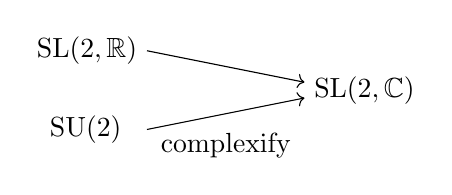
\begin{tikzpicture}
          \node[left] at (0,0.5) {$\SL(2, \mathbb{R})$};
          \node[left] at (-0.2,-0.5) {SU$(2)$};
          \node[right] at (2,0) {$\SL(2,\mathbb{C})$};
          \draw[->] (0,0.5)--(2,0.1);
          \draw[->] (0,-0.5)--(2,-0.1);
          \node at (1,-0.7) {complexify};
        \end{tikzpicture}
      \end{center}
      We can interpret the "real forms" of $\SL(2, \mathbb{C})$ as "slices" of some complex group. However, this does not mean that the real version of these groups are equal. That is, 
      \begin{equation}
        \SL(2, \mathbb{R}) \neq \text{SU}(2)
      \end{equation}

    \subsubsection{Lie Algebra of SO(3)}

      It is easy to see that for SO$(2)$, it is easy to see that its Lie algebra $\mathfrak{so}(2)$ has 
      \begin{equation}
        \bigg\{ \begin{pmatrix}
        0&-1\\1&0
        \end{pmatrix}\bigg\}
      \end{equation}
      as its only basis, since 
      \begin{equation}
        exp  \bigg( \begin{pmatrix}
        0&-1\\1&0
        \end{pmatrix} \theta \bigg) = \begin{pmatrix}
        \cos{\theta} & - \sin{\theta} \\
        \sin{\theta} & \cos{\theta}
        \end{pmatrix}
      \end{equation}
      meaning that the dimension of SO$(2)$ is $1$. By adding a component, we can get a rotation in $\mathbb{R}^3$. 
      \begin{align*}
        & R_x = \begin{pmatrix}0&0&0\\0&0&-1\\0&1&0\end{pmatrix} \implies e^{R_x} = \begin{pmatrix}
        1&0&0\\ 0&\cos{\theta}&-\sin{\theta}\\0&\sin{\theta}&\cos{\theta}
        \end{pmatrix}\\
        & R_y = \begin{pmatrix}0&0&1\\0&0&0\\-1&0&0\end{pmatrix} \implies e^{R_y} = \begin{pmatrix}
        \cos{\theta} & 0 & -\sin{\theta}\\ 0&1&0 \\
        \sin{\theta}& 0 & \cos{\theta} \end{pmatrix} \\
        & R_z = \begin{pmatrix}0&-1&0\\1&0&0\\0&0&0\end{pmatrix} \implies e^{R_z} = \begin{pmatrix}
        \cos{\theta} & -\sin{\theta} & 0\\
        \sin{\theta}& \cos{\theta} & 0 \\ 0 & 0 & 1\end{pmatrix}
      \end{align*}
      That is, $e^{R_x}, e^{R_y}$, and $e^{R_z}$ generates a rotation around the $x, y$, and $z$ axis, respectively, which completely generates the group SO$(3)$. Therefore, the Lie algebra $\mathfrak{so}(3)$ consists of the basis 
      \begin{equation}
        \{R_x, R_y, R_z\}
      \end{equation}
      The bracket structure (again, defined as the commutator) of this Lie algebra is 
      \begin{align*}
        & [R_x, R_y] = R_z \\
        & [R_y, R_z] = R_x \\
        & [R_z, R_x] = R_y
      \end{align*}
      which is similar to the brakcet structure of $\mathfrak{su}(2)$. Therefore, SO$(3)$ and SU$(2)$ have the \textit{same} Lie algebra, which is the algebra of dimension 3 with the same bracket structure. Note that Lie algebras are uniquely determined by the bracket structure and dimension. However, having the same Lie algebra does not imply that the groups are identical (obviously) nor isomorphic. For example, 
      \begin{equation}
        exp(2\pi R_z) = \begin{pmatrix}
        \cos{2\pi} & -\sin{2\pi} & 0 \\
        \sin{2\pi} & \cos{2\pi} & 0 \\
        0 & 0 & 1
        \end{pmatrix} = I
      \end{equation}
      while 
      \begin{equation}
        exp(2\pi A_z) = 
        exp(-i \pi \sigma_z) = exp \bigg(-i \pi \begin{pmatrix}
        1&0\\0&-1
        \end{pmatrix} \bigg) = -I
      \end{equation}
      There is discrepancy by a factor of $-1$. In fact, it turns out that
      \begin{equation}
        \text{SO}(3) = \frac{\text{SU}(2)}{\pm I}
      \end{equation}
      We justify this in the following way. Let $v \in \mathbb{R}^3$ have components $(x, y, z)$. Consider
      \begin{equation}
        M = x \sigma_x + y \sigma_y + z \sigma_z
      \end{equation}
      $M$ is clearly traceless and $M^\dagger = M$. Now, let $S \in$ SU$(2)$ and let $M^\prime = S^{-1} M S$. Then, $\Tr{M^\prime} = \Tr{S^{-1} M S} = \Tr{M} = 0$ and $(M^\prime)^\dagger = (S^{-1} M S)^\dagger = S^\dagger M^\dagger (S^{-1})^\dagger = S^{-1} M S = M^\prime$. Therefore, since $M^\prime$ is self adjoint and traceless, it can be expressed in the form
      \begin{equation}
        x^\prime \sigma_x + y^\prime \sigma_y + z^\prime \sigma_z
      \end{equation}
      for some $(x^\prime, y^\prime, z^\prime)$. Now, since 
      \begin{equation}
        M^2 = (-x^2 - y^2 - z^2) I
      \end{equation}
      we have 
      \begin{align*}
        (M^\prime)^2 & = S^{-1} M^2 S = (-x^2 - y^2 - z^2) I \\
        & = (-x^{\prime 2} - y^{\prime 2} - z^{\prime 2}) I 
      \end{align*}
      So, $x^2 + y^2 + z^2 = x^{\prime 2} + y^{\prime 2} + z^{\prime 2}$, implying that the lengths of $v$ stayed the same. (The proof of linearity of $S$ is easy.) Therefore, the transformation $M \mapsto M^\prime$, i.e. $(x, y, z) \mapsto (x^\prime, y^\prime, z^\prime)$ is a linear transformation preserving length in $\mathbb{R}^3$ (with respect to the usual inner product and norm) $\implies$ it is in SO$(3)$. If we have
      \begin{equation}
        S  = \begin{pmatrix}
        -1&0\\0&-1
        \end{pmatrix}
      \end{equation}
      then $M^\prime = M$, which explains why SO$(3)$ is a coset deviating by both $I$ and $-I$. Visually, if we let SU$(2)$ be a circle, points that are diametrically opposite of each other are "equivalent" in SO$(3)$. That is, SU$(2)$ is a three-dimensional sphere, and $g$ and $-g$ are identified onto the same element in SO$(3)$. This map
      \begin{equation}
        \rho: \text{SU}(2) \longrightarrow \text{SO}(3)
      \end{equation}
      in which 2 points are mapped to 1 point is a surjective map with
      \begin{equation}
        \ker{\rho} = \{I, -I\}
      \end{equation}
      \begin{center}
        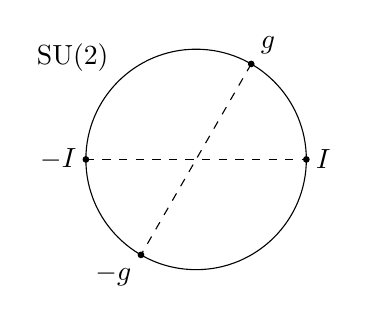
\begin{tikzpicture}[scale=0.7]
          \draw (0,0) circle (2);
          \draw[fill] (2,0) circle (0.05);
          \draw[fill] (-2,0) circle (0.05);
          \node[right] at (2,0) {$I$};
          \node[left] at (-2,0) {$-I$};
          \draw[fill] (1,1.732) circle (0.05);
          \draw[fill] (-1,-1.732) circle (0.05);
          \node[above right] at (1, 1.732) {$g$};
          \node[below left] at (-1, -1.732) {$-g$};
          \draw[dashed] (-2,0)--(2,0);
          \draw[dashed] (1, 1.732)--(-1, -1.732);
          \node[above left] at (-1.414, 1.414) {SU$(2)$};
        \end{tikzpicture}
      \end{center}

      We can in fact explicitly describe exponential map from $\mathfrak{so}(3)$ to SO$(3)$ with the following lemma. 

      \begin{lemma}[Rodrigues' Formula]
        The exponential map $exp: \mathfrak{so}(3) \longrightarrow$ SO$(3)$ is defined by 
        \begin{equation}
          e^A = \cos{\theta} I_3 + \frac{\sin{\theta}}{\theta} A + \frac{(1 - \cos{\theta})}{\theta^2} B
        \end{equation}
        where 
        \begin{equation}
          A = \begin{pmatrix}
          0&-c&b\\c&0&-a\\-b&a&0
          \end{pmatrix}, B = \begin{pmatrix}
          a^2&ab&ac\\ab&b^2&bc\\ac&bc&c^2
          \end{pmatrix}
        \end{equation}
        This formula has many applications in kinematics, robotics, and motion interpolation. 
      \end{lemma}

      \begin{theorem}
      The Lie algebras for the following classical Lie groups are summarized as follows. 
      \begin{enumerate}
        \item $\mathfrak{sl}_n \mathbb{R}$ is the real vector space of real $n \times n$ matrices with null trace.
        \item $\mathfrak{so}(n)$ is the real vector space of real $n \times n$ skew-symmetric matrices. 
        \item $\mathfrak{gl}_n \mathbb{R}$ is the real vector space of all real $n \times n$ matrices.
        \item $\mathfrak{o}(n) = \mathfrak{o}(n)$
      \end{enumerate}
      \end{theorem}
      Note that the corresponding groups $\GL(n, \mathbb{R}), \SL(n, \mathbb{R}), \mathfrak{gl}_n \mathbb{R}, \mathfrak{sl}_n \mathbb{R}$ are Lie groups, meaning that they are smooth real manifolds. We can view each of them as smooth real manifolds embedded in the $n^2$ dimensional vector space of real matrices, which is isomorphic to $\mathbb{R}^{n^2}$. 

      \begin{theorem}
        The Lie algebras $\mathfrak{gl}_ \mathbb{R}, \mathfrak{sl}_n \mathbb{R}, \mathfrak{o}(n), \mathfrak{so}(n)$ are well-defined, but only 
        \begin{equation}
          exp: \mathfrak{so}(n) \longrightarrow \text{SO}(n)
        \end{equation}
        is surjective. 
      \end{theorem}

      \begin{theorem}
        The Lie algebras for the following classical Lie groups are summarized as follows. 
        \begin{enumerate}
          \item $\mathfrak{sl}_2 \mathbb{C}$ is the real (or complex) vector space of traceless complex $n \times n$ matrices. 
          \item $\mathfrak{u}(n)$ is the real vector space of complex $n \times n$ skew-Hermitian matrices. 
          \item $\mathfrak{su}(n) = \mathfrak{u} \cap \mathfrak{sl}_2 \mathbb{C}$. It is also a real vector space. 
          \item $\mathfrak{gl}_n \mathbb{C}$ is the real (or complex) vector space of complex $n \times n$ matrices. 
        \end{enumerate}
        Note that even though the matrices in these Lie algebras have complex coefficients, we have assigned them to be in a \textit{real} vector space, which means that we are only allowed to take real linear combinations of these elements. That is, the field we are working over is $\mathbb{R}$ (this does not contradict any of the axioms for vector spaces). For example an element $A$ in $\mathfrak{u}(n)$ or $\mathfrak{su}(n)$ must be anti-self adjoint, but $iA$ is self adjoint. 
      \end{theorem}

      Similarly, the Lie groups 
      \begin{equation}
        \GL(n, \mathbb{C}), \SL(n, \mathbb{C}), \mathfrak{gl}_n \mathbb{C}, \mathfrak{sl}_n \mathbb{C}
      \end{equation}
      are also smooth real manifolds embedded in Mat$(n, \mathbb{C}) \simeq \mathbb{C}^{n^2} \simeq \mathbb{R}^{2 n^2}$. So, we can view these four groups as manifolds embedded in $\mathbb{R}^{2 n^2}$. 

      Note some of the similarities and differences between the real and complex counterparts of these Lie groups and algebras. 
      \begin{enumerate}
        \item $\mathfrak{o}(n) = \mathfrak{so}(n)$, but $\mathfrak{u}(n) \neq \mathfrak{su}(n)$. 
        \item $exp: \mathfrak{gl}_n \mathbb{R} \longrightarrow \GL(n, \mathbb{R})$ is not surjective, but $exp: \mathfrak{gl}_n \mathbb{C} \longrightarrow \GL(n, \mathbb{C})$ is surjective due to the spectral theorem and surjectivity of $exp: \mathbb{C} \longrightarrow \mathbb{C}^*$.
        \item The exponential maps $exp: \mathfrak{u}(n) \longrightarrow \text{U}(n)$ and $exp: \mathfrak{su}(n) \longrightarrow \text{SU}(n)$ are surjective. 
        \item Still, $exp: \mathfrak{sl}_2 \mathbb{C} \longrightarrow \SL(2, \mathbb{C})$ is not surjective. This will be proved now. 
      \end{enumerate}

      \begin{theorem}
        $exp: \mathfrak{sl}_2 \mathbb{C} \longrightarrow \SL(2, \mathbb{C})$ is not surjective. 
      \end{theorem}
      \begin{proof}
        Given $M \in \SL(n, \mathbb{C})$, assume that $M = e^A$ for some matrix $A \in \mathfrak{sl}_2 \mathbb{C}$. Putting $A$ into the Jordan Normal Form $J = N A N^{-1}$ means that $J$ can either be of form
        \begin{equation}
          J = \begin{pmatrix}
          0&1\\0&0
          \end{pmatrix}, \begin{pmatrix}
          \lambda&0\\0&-\lambda
          \end{pmatrix} \implies e^J = \begin{pmatrix}
          1&1\\0&1
          \end{pmatrix}, \begin{pmatrix}
          e^\lambda&0\\0&e^{-\lambda}
          \end{pmatrix}
        \end{equation}
        which is also in JNF in $\SL(2, \mathbb{C})$. But a matrix $P \in \SL(2, \mathbb{C})$ may exist with JNF of 
        \begin{equation}
          K = \begin{pmatrix}
          -1&1\\0&-1
          \end{pmatrix}
        \end{equation}
        which is not one of the 2 forms. So, $K \not\in \im{exp} \implies exp$ is not surjective. 
      \end{proof}

      \begin{theorem}
      The exponential maps 
      \begin{align*}
        & exp: \mathfrak{u}(n) \longrightarrow \text{U}(n) \\
        & exp: \mathfrak{su}(n) \longrightarrow \text{SU}(n)
      \end{align*}
      are surjective. 
      \end{theorem}

    \subsubsection{Lie Algebra of SE(n)}

      Recall that the group of affine rigid isometries is denoted SE$(n)$. That is, 
      \begin{equation}
        \text{SE}(n) \equiv \text{SO}(n) \ltimes \text{Tran}\,\mathbb{R}^n
      \end{equation}
      We can define the matrix representation of this affine transformation as such. Given an element $g \in$ SE$(n)$ such that
      \begin{equation}
        g(x) \equiv R x + U, \; R \in \text{SO}(n), U \in \text{Tran}\, \mathbb{R}^n 
      \end{equation}
      we define the representation
      \begin{equation}
        \rho: \text{SE}(n) \longrightarrow \GL(n+1, \mathbb{R}), \rho(g) \equiv \begin{pmatrix}
        R&U\\0&1
        \end{pmatrix}
      \end{equation}
      where $R$ is a real $n\times n$ matrix in SO$(n)$ and $U$ is a real $n$-vector in Tran$\,\mathbb{R}^n \simeq \mathbb{R}^n$. We would then have
      \begin{equation}
        \rho(g) \begin{pmatrix}
        x\\1
        \end{pmatrix} \equiv \begin{pmatrix}
        R&U\\0&1
        \end{pmatrix} \begin{pmatrix}
        x\\1
        \end{pmatrix} = \begin{pmatrix}
        R x + U\\1
        \end{pmatrix} \in \mathbb{R}^{n+1}
      \end{equation}

      Clearly, SE$(n)$ is a Lie group, and the matrix representation $\varrho$ of its Lie algebra $\mathfrak{se}(n)$ can be defined as the vector space of $(n+1) \times (n+1)$ matrices of the block form 
      \begin{equation}
        A = \begin{pmatrix}
        \Omega & U \\0 & 0
        \end{pmatrix}
      \end{equation}
      where $\Omega$ is an $n \times n$ skew-symmetric matrix and $U \in \mathbb{R}^n$. Note that there are two different exponential maps here: one belonging to the abstract Lie group SE$(n)$ and another belonging to the concrete, matrix group $\GL(n+1, \mathbb{R})$. This can be represented with the commutative diagram. 
      \[\begin{tikzcd}
      \mathfrak{se}(n) \arrow{r}{exp} \arrow{d}{\varrho} & SE(n) \arrow{d} {\rho}\\
      \mathfrak{gl}_{n+1} \mathbb{R} \arrow{r}{exp} & \GL(n+1, \mathbb{R})
      \end{tikzcd}\]

      \begin{lemma}
        Given any $(n+1) \times (n+1)$ matrix of form 
        \begin{equation}
          A = \begin{pmatrix}
           \Omega & U \\0&0
          \end{pmatrix}
        \end{equation}
        where $\Omega$ is any matrix and $U \in \mathbb{R}^n$, 
        \begin{equation}
          A^k = \begin{pmatrix}
          \Omega^k & \Omega^{k-1} U \\0&0
          \end{pmatrix}
        \end{equation}
        where $\Omega^0 = I_n$, which implies that
        \begin{equation}
          e^A = \begin{pmatrix}
          e^\Omega & V U \\ 0 & 1
          \end{pmatrix}, \; V = I_n + \sum_{k \geq 1} \frac{\Omega^k}{(k+1)!}
        \end{equation}
      \end{lemma}

      \begin{theorem}
        The exponential map
        \begin{equation}
          exp: \mathfrak{se}(n) \longrightarrow SE(n)
        \end{equation}
        is well-defined and surjective. 
      \end{theorem}

  \subsection{Representations of Lie Groups and Lie Algebras}

    Let $\mathcal{G}$ be an abstract group and let
    \begin{equation}
      \rho: \mathcal{G} \longrightarrow \GL(V)
    \end{equation}
    be the representation of $\mathcal{G}$. Then, let $\mathfrak{g}$ be the Lie algebra of $\mathcal{G}$, and $\mathfrak{gl}(V)$ be the Lie algebra of $\GL(V)$. Then, $\rho$ induces another homomorphism 
    \begin{equation}
      \varrho: \mathfrak{g} \longrightarrow \mathfrak{gl}(V)
    \end{equation}
    where the bracket structure (in this case, the comutator in the matrix algebra) is preserved. 
    \begin{equation}
      \varrho([X,Y]) = [\varrho(X), \varrho(Y)]
    \end{equation}
    We can visualize this induced homomorphism with the following commutative diagram, which states that $\rho \circ exp = exp \circ \varrho$. 

    \[\begin{tikzcd}
    \mathcal{G} \arrow{r}{\rho} & \GL(V)\\
    \mathfrak{g} \arrow{u}{exp} \arrow{r}{\varrho} & \mathfrak{gl}(V) \arrow{u}{exp}
    \end{tikzcd}\]

    Note that there are very crucial differences between $\rho$ and $\varrho$. First, $\rho$ is a homomorphism between \textit{groups}, while $\varrho$ is a homomorphism between \textit{vector spaces}. Additionally, $\GL(V)$ is a group, not a linear space, while $\mathfrak{gl}(V)$ is a linear space. Finally, note that $\GL(V)$ is restricted to only matrices with nonzero determinants, while the elements of $\mathfrak{gl}(V)$ can be any matrix. 

    \begin{example}
      The representation of SE$(n)$ to $\GL(n+1 \mathbb{R}$ and $\mathfrak{se}(n)$ to $\mathfrak{gl}_{n+1} \mathbb{R}$ induces the second homomorphism $\varrho: \mathfrak{gl}_{n+1} \mathbb{R} \longrightarrow \GL(n+1, \mathbb{R})$. 
    \end{example}

    \begin{definition}
      The direct sum of representations is a representation. That is, if $U$ is a representation and $V$ is a representation, then $U \oplus V$ is a representation. That is, if 
      \begin{equation}
        \rho_1: \mathcal{G} \longrightarrow U, \; \rho_1 (g) = \begin{pmatrix}
        u_1&u_2\\u_3&u_4
        \end{pmatrix}
      \end{equation}
      and
      \begin{equation}
        \rho_2: \mathcal{G} \longrightarrow V, \; \rho_2 (g) = \begin{pmatrix}
        v_1 & v_2 \\ v_3 & v_4
        \end{pmatrix}
      \end{equation}
      are two representations of the same group element $g \in \mathcal{G}$, then 
      \begin{equation}
        (\rho_1 \oplus \rho_2): \mathcal{G} \longrightarrow (U \oplus V), \;(\rho_1 \oplus \rho_2) (g) = \begin{pmatrix}
        u_1 & u_2 & 0 & 0 \\
        u_3 & u_4 & 0 & 0 \\
        0 & 0 & v_1 & v_2 \\
        0 & 0 & v_3 & v_4 
        \end{pmatrix}
      \end{equation}
      is a bigger representation of $g$ in $U \oplus V$. 
    \end{definition}

    \begin{definition}
      $V$ is irreducible if the only subspaces which are representations are only $V$ and $\{0\}$. 
    \end{definition}

    For our case, we will consider that any representation can be written as a direct sum of irreducible representations. We will now proceed to find an irreducible representation of $\mathfrak{sl}_2 \mathbb{C}$. This means that we want to find the smallest (lowest dimensional) vector space $V$ such that there exists a representation
    \begin{equation}
      \varrho: \mathfrak{sl}_2 \mathbb{C} \longrightarrow \mathfrak{gl}(V)
    \end{equation}
    We will write, as shorthand notation, that 
    \begin{equation}
      H = \varrho(H), X = \varrho(X), Y = \varrho(Y)
    \end{equation}
    Clearly, $H, X, Y \in \mathfrak{gl}(V) \simeq \mathfrak{gl}(\mathbb{C}^n)$. By the spectral theorem, we can find an orthonormal basis of eigenvectors $e_1, e_2, ..., e_n$ of the mapping $H$ such that
    \begin{equation}
      H e_i = \lambda_i e_i, \; \lambda_i \in \mathbb{C}
    \end{equation}
    Since $[H,X] = 2X$, it follows that
    \begin{equation}
      HX e_i - X H e_i = 2X e_i \implies H (X e_i) = (\lambda_i + 2) (X e_i)
    \end{equation}

    $\implies Xe_i$ for all $i = 1, 2, ..., n$ are also eigenvectors of $H$ with eigenvalue $(\lambda_i + 2)$, or $X e_i = 0$. So, $X$ is a "ladder operator" that maps each eigenvector $e_i$ with eigenvalue $\lambda_i$ to a different eigenvector $e_j$ with eigenvalue $\lambda_j = \lambda_i + 2$. Having nowhere to be mapped to, the eigenvector with the largest eigenvalue (which must exist since $V$ is finite dimensional) will get mapped to the $0$ vector by $X$. Let us denote this eigenvector having the maximum eigenvalue $m$, as $v_m$. 

    Similarly, $[H,Y] = -2Y$ implies that
    \begin{equation}
      HY e_i - YH e_i = -2Y e_i \implies H(Y e_i) = (\lambda_i - 2)(Y e_i)
    \end{equation}

    implying that $Y$ maps each eigenvector $e_i$ with eigenvaue $\lambda_i$ to another eigenvector $e_j$ with eigenvalue $\lambda_j = \lambda_i - 2$, except for the eigenvector with smallest eigenvalue, which gets mapped to $0$. Since $Y$ clearly maps each eigenvector to a different eigenvector that has a strictly decreasing eigenvalue, we can construct a basis of $V$ to be
    \begin{equation}
      \{v_m, Y v_m, Y^2 v_m, Y^3 v_m, ..., Y^{n-1} v_m\}
    \end{equation}
    (remember that $Y^n v_m = 0$). So, elements of $\mathfrak{sl}_2 \mathbb{C}$ acts on the space $V$ with basis above. To continue, we introduce the following proposition. 

    \begin{proposition}
      \begin{equation}
        X Y^j v_m = j(m-j+1) Y^{j-1} v_m
      \end{equation}
    \end{proposition}
    \begin{proof}
      By induction on $j$ using bracket relations.
    \end{proof}

    $V$ is $n$-dimensional. Since $Y^n v_m = 0$ and $Y^{n-1} v_m \neq 0$, we use the proposition above to get
    \begin{equation}
      0 = X Y^n v_m = n (m-n+1) Y^{n-1} v_m \implies m-n+1=0
    \end{equation}
    So, $n = m+1$, which means that the eigenvalues of $H$ are
    \begin{equation}
      m, m-2, m-4, \ldots, m - 2(n-1) = -m
    \end{equation}

    and we are done. We now classify the 1, 2, and 3 dimensional irreducible representations of $\mathfrak{sl}_2 \mathbb{C}$. 
    \begin{enumerate}
      \item When $n = 1$ (i.e. dimension is 1), $m = n-1 = 0$, meaning that the greatest (and only) eigenvalue is $0$. That is, 
        \begin{equation}
          H v_0 = 0,\; X v_0 = 0,\; Y v_0 = 0
        \end{equation}
      which is the trivial representation of $\mathfrak{sl}_2 \mathbb{C}$. Explicitly, we can completely define the representation (which is a linear homomorphism) with the three equations. 
      \begin{equation}
        \varrho(H) = (0),\; \varrho(X) = (0),\; \varrho(Y) = (0)
      \end{equation}

      \item When $n = 2$ and $m=1$. We now look for a 2 dimensional irreducible representation. The eigenvalues are $1$ and $-1$, with $\{v_1, v_{-1}\}$ as a basis of 2 dimensional space $V$. Then we have 
        \begin{align*}
          & Hv_1 = v_1, \; Hv_{-1} = - v_{-1} \\
          & X v_1 = 0, \; X v_{-1} = v_1 \\
          & Y v_1 = v_{-1}, \; Y v_{-1} = 0
        \end{align*}
      which explicitly translates to the representation $\varrho$ being defined
      \begin{equation}
        \varrho(H) = \begin{pmatrix}
        1&0\\0&-1
        \end{pmatrix}, \; \begin{pmatrix}
        0&1\\0&0
        \end{pmatrix}, \; \begin{pmatrix}
        0&0\\1&0
        \end{pmatrix}
      \end{equation}

      \item When $n=3 \implies m=2$, the basis is $\{v_{-2}, v_0, v_2\}$ with eigenvalues $2, 0, -2$, and the irreducible representation $\varrho$ is defined
        \begin{equation}
          \varrho(H) = \begin{pmatrix}
          2&&\\&0&\\&&-2
          \end{pmatrix}, \varrho(Y) = \begin{pmatrix}
          0&0&0\\1&0&0\\0&1&0
          \end{pmatrix}, \varrho(X) = \begin{pmatrix}
          0&1&0\\0&0&1\\0&0&0
          \end{pmatrix}
        \end{equation}

      \item The same process continues on for $n=4, 5, ...$, and this entirely classifies the irreducible representations of $\mathfrak{sl}_2 \mathbb{C}$. 
    \end{enumerate}

    \subsubsection{Tensor Products of Group Representations}

      \begin{definition}
        If $V$ and $W$ are two different representations of a group $\mathcal{G}$, then we know that $V \oplus W$ is also a representation of $\mathcal{G}$. Furthermore, the tensor product space $V \otimes W$ also defines a representation of $\mathcal{G}$. That is, given representations
        \begin{align*}
          & \rho_V: \mathcal{G} \longrightarrow \GL(V) \\
          & \rho_W: \mathcal{G} \longrightarrow \GL(W)
        \end{align*}
        The homomorphism 
        \begin{equation}
          \rho_V \otimes \rho_W: \mathcal{G} \longrightarrow \GL(V \otimes W)
        \end{equation}
        is also a representation of $\mathcal{G}$, which is defined
        \begin{equation}
          (\rho_V \otimes \rho_W)(g) (v \otimes w) \equiv \rho_V (g) (v) \otimes \rho_W (g) (w)
        \end{equation}
        or represented in shorthand notation, 
        \begin{equation}
          g(v \otimes w) \equiv (g v) \otimes (g w)
        \end{equation}
        We know that exp$(H)$ acts on $V$ and $W$ since it is an element of $\GL(V)$ and $\GL(W)$. This means that
        \begin{equation}
          exp(H)(v \otimes w) \equiv \big( exp(H)(v)\big) \otimes \big( exp(H)(w)\big)
        \end{equation}
        If $H$ ($= \rho_V (H)$ or $\rho_W(H)$) has an eigenvalue $\lambda$ on $v$ in $V$ and eigenvalue $\mu$ on $w$ in $W$, then 
        \begin{equation}
          exp(H) (v \otimes w) = (e^\lambda v) \otimes (e^\mu w) = e^{\lambda + \mu} v \otimes w
        \end{equation}
        That is, eigenvalues of $H$ \textit{add} on tensor products. 
      \end{definition}

      \begin{example}
        Recall that the $2$ dimensional representation $V$ of $\mathfrak{sl}_2 \mathbb{C}$ has eigenvalues $1$ and $-1$ (with corresponding eigenvectors $e_1$ and $e_{-1}$). So, $V \otimes V$ has eigenvalues 
        \begin{align*}
          & (-1) + (-1) = -2, \;\; (-1) + 1 = 0 \\
          & 1 + (-1) = 0, \;\; 1 + 1 = 2
        \end{align*}
        Therefore, the eigenvalues of $V \otimes V$ is $-2$ (geometric multiplicity of 1), $0$ (geometric multiplicity of 2), and $2$ (geometric multiplicity of 1), (Notation-wise, the $n$-dimensional irreducible representation of $\mathfrak{sl}_2 \mathbb{C}$ is denoted $\mathbf{n}$.) which means that
        \begin{equation}
          \mathbf{2} \otimes \mathbf{2} = \mathbf{3} \oplus \mathbf{1}
        \end{equation}
        We can decompose $V \otimes V$ into its symmetric and exterior power components. Sym$^2 V$ has basis (of eigenvectors)
        \begin{equation}
          \{e_{-1} \odot e_{-1}, \; e_{-1} \odot e_1, \; e_1 \odot e_1\}
        \end{equation}
        where the corresponding eigenvalues are $-2$, $0$, and $2$, respectively. So, $\dim{Sym^2 V} = 3$, which means that $Sym^2 V = \mathbf{3}$. As for the exterior power component of $V$, $\Lambda^2 V$ has basis 
        \begin{equation}
          \{e_{-1} \wedge e_1\}
        \end{equation}
        with eigenvalue $= 0 \implies \dim{\Lambda^2 V} = 1$, meaning that $\Lambda^2 V = \mathbf{1}$. Therefore, 
        \begin{equation}
          V \otimes V = Sym^2 V \oplus \Lambda^2 V = \mathbf{3} \oplus \mathbf{1}
        \end{equation}
      \end{example}

  \subsection{Topological Decompositions of Lie Groups}

    \begin{definition}
      Let us define 
      \begin{enumerate}
        \item S$(n)$ is the vector space of real, symmetric $n \times n$ matrices. 
        \item SP$(n)$ is the set of symmetric, positive semidefinite matrices. 
        \item SPD$(n)$ is the set of symmetric, positive definite matrices. 
      \end{enumerate}
      Note that SP$(n)$ and SPD$(n)$ are not even vector spaces at all. 
    \end{definition}

    \begin{lemma}
      The exponential map 
      \begin{equation}
        exp: S(n) \longrightarrow SPD(n)
      \end{equation}
      is a homeomorphism. One may be tempted to call S$(n)$ the Lie algebra of SPD$(n)$, but this is not the case. S$(n)$ is not even a Lie algebra since the commutator is not algebraically closed. Furthermore, SPD$(n)$ is not even a multiplicative group (since matrix multiplication is not closed). 
    \end{lemma}

    Recall from linear algebra the Polar Decomposition. We express this result in a slightly modified way. 

    \begin{theorem}[Polar Decomposition]
      Given a Euclidean space $\mathbb{E}^n$ and any linear endomorphism $f$ of $\mathbb{E}^n$, there are two positive definite self-adjoint linear maps $h_1, h_2 \in$ End$(\mathbb{E}^n)$ and $g \in$ O$(n)$ such that
      \begin{equation}
        f = g \circ h_1 = h_2 \circ g
      \end{equation}
      That is, such that $f$ can be decomposed into the following compositions of functions that commute. 

      \[\begin{tikzcd}
      \mathbb{E}^n \arrow{r}{h_2} & \mathbb{E}^n \\
      \mathbb{E}^n \arrow{u}{g} \arrow{ur}{f} \arrow{r}{h_1} & \mathbb{E}^n \arrow{u}{g}
      \end{tikzcd}\]

      This means that there is a bijection between $Mat(n, \mathbb{R})$ and $O(n) \times SP(n)$. If $f$ is an automorphism, then this decomposition is unique. 
    \end{theorem}

    \begin{corollary}
      The two topological groups are homeomorphic. 
      \begin{equation}
        GL(n, \mathbb{R}) \cong O(n) \times SPD(n)
      \end{equation}
    \end{corollary}

    \begin{corollary}
      For every invertible real matrix $A \in GL(n, \mathbb{R})$, there exists a unique orthogonal matrix $R$ and unique symmetric matrix $S$ such that
      \begin{equation}
        A = R e^S
      \end{equation}
      $\implies$ there is a bijection between $\GL(n, \mathbb{R})$ and $O(n) \times S(n) \simeq \mathbb{R}^{n(n+1)/2}$. Moreover, they are homeomorphic. That is, 
      \begin{equation}
        \GL(n, \mathbb{R}) \simeq O(n) \times S(n) \simeq O(n) \times \mathbb{R}^{n(n+1)/2}
      \end{equation}
      This essentially reduces the study of $\GL(n, \mathbb{R})$ to the study of $O(n)$, which is nice since $O(n)$ is compact. 
    \end{corollary}

    \begin{corollary}
      Given a real matrix $A$, if $\det{A} > 0$, then we can decompose $A$ as
      \begin{equation}
        A = R e^S
      \end{equation}
      where $R \in SO(n)$ and $S \in S(n)$. 
    \end{corollary}

    \begin{corollary}
      There exists a bijection between
      \begin{equation}
        \SL(n, \mathbb{R}) \text{ and } SO(n) \times (S(n) \cap \mathfrak{sl}_n \mathbb{R})
      \end{equation}
    \end{corollary}
    \begin{proof}
      $A \in \SL(n, \mathbb{R}) \implies 1 = \det{A} = \det{R} \det{e^S} = \det{e^S} \implies \det{e^S} = e^{\Tr{S}} = 1 \implies \Tr{S} = 0 \implies S \in$ S$(n) \cap \mathfrak{sl}_n \mathbb{R}$. 
    \end{proof}

    \begin{definition}
      Let us define
      \begin{enumerate}
        \item H$(n)$ is the real vector space of $n \times n$ Hermitian matrices. 
        \item HP$(n)$ is the set of Hermitian, positive semidefinite $n \times n$ matrices. 
        \item HPD$(n)$ is the set of Hermitian, positive definite $n \times n$ matrices. 
      \end{enumerate}
      Similarly, HP$(n)$ and HPD$(n)$ are not vector space. They are just sets. 
    \end{definition}

    \begin{lemma}
      The exponential mapping
      \begin{equation}
        exp: H(n) \longrightarrow HPD(n)
      \end{equation}
      is a homeomorphism. 
    \end{lemma}

    However again, HPD$(n)$ is not a Lie group (multiplication is not algebraically closed) nor is H$(n)$ a Lie algebra (commutator is not algebraically closed). By the polar form theorem of complex $n \times n$ matrices, we have a (not necessarily unique) bijection between
    \begin{equation}
      \text{Mat}(n, \mathbb{C}) \text{ and } U(n) \times HP(n)
    \end{equation}
    which implies that
    \begin{equation}
      \GL(n, \mathbb{C}) \cong U(n) \times HPD (n)
    \end{equation}

    \begin{corollary}
      For every complex invertible matrix $A$, there exists a unique decomposition
      \begin{equation}
        A = U e^S
      \end{equation}
      where $U \in U(n)$ and $S \in H(n)$, which implies that the following groups are homeomorphic. 
      \begin{align*}
        \GL(n, \mathbb{C}) & \cong U(n) \times H(n) \\
        & \cong U(n) \times \mathbb{R}^{n^2}
      \end{align*} 
      This essentially reduces the study of $\GL(n, \mathbb{C})$ to that of U$(n)$. 
    \end{corollary}

    \begin{corollary}
      There exists a bijection between 
      \begin{equation}
        \SL(n, \mathbb{C}) \text{ and } SU(n) \times (H(n) \cap \mathfrak{sl}_n \mathbb{C})
      \end{equation}
    \end{corollary}
    \begin{proof}
      Similarly, when $A = U e^S$, we know that $|\det{U}| = 1$ and $\Tr{S}$ is real (since by the Spectral theorem, every self adjoint matrix has a real spectral decomposition). Since $S$ is Hermitian, this implies that $\det{e^S} > 0$. If $A \in \SL(n, \mathbb{C})$, then $\det{A} = 1 \implies \det{e^S} = 1 \implies S \in H(n) \cap \mathfrak{sl}_n \mathbb{C}$. 
    \end{proof}

  \subsection{Linear Lie Groups}

    We will assume that the reader has the necessary background knowledge in manifolds, chart mappings, diffeomorphisms, tangent spaces, and transition mappings. 

    Recall that the algebra of real $n \times n$ matrices Mat$(n, \mathbb{R})$ is bijective to $\mathbb{R}^{n^2}$, which is a topological space. Therefore, this bijection 
    \begin{equation}
      i:(\mathbb{R}^{n^2}, \tau_E) \longrightarrow \text{Mat}(n, \mathbb{R})
    \end{equation}
    induces a topology on Mat$(n, \mathbb{R})$, defined 
    \begin{equation}
      \tau_M \equiv \{U \in \text{Mat}(n, \mathbb{R}) \; | \; e^{-1} (U) \in \tau_E\}
    \end{equation}
    With this, consider the subset
    \begin{equation}
      \GL(n, \mathbb{R}) \subset \text{Mat}(n, \mathbb{R})
    \end{equation}
    where
    \begin{equation}
      \GL(n, \mathbb{R}) \equiv \{x \in \text{Mat}(n, \mathbb{R}) \;|\; \det{x} \neq 0\}
    \end{equation}
    This set, as we expect, is a multiplicative group. 

    \begin{definition}
      The \textit{general linear group}, denoted $\GL(n, \mathbb{R})$ is the set of $n \times n$ matrices with nonzero determinant. The more technical definition is that $\GL(n, \mathbb{R})$ is really just the automorphism group of $\mathbb{R}^n$, 
      \begin{equation}
        \GL(n, \mathbb{R}) \equiv \text{Aut}(\mathbb{R}^n)
      \end{equation}
      but it is customary to assume a basis on $\mathbb{R}^n$ in order to realize $\GL(n, \mathbb{R})$ as a matrix group. Note that the procedure of assuming a basis on $\mathbb{R}^n$ is the same as defining a representation of the abstract group $\GL(n, \mathbb{R})$. Both assigns a real $n \times n$ matrix to each element of $\GL(n, \mathbb{R})$. 
    \end{definition}

    In this way, we can view $\GL(n, \mathbb{R})$ as a topological space in $\mathbb{R}^{n^2}$, and it is fine to interpret $\GL(n, \mathbb{R})$ as a matrix group rather than an abstract group. 

    Since the matrix representation of $\GL(n, \mathbb{R})$ is always well defined, the abstract subgroups of $\GL(n, \mathbb{R})$, which are $\SL(n, \mathbb{R}), O(n)$, and $SO(n)$, also have well defined matrix representations (that we are all familiar with). Additionally, since there exists a bijection
    \begin{equation}
      \text{Mat}(n, \mathbb{C}) \cong \mathbb{C}^{n^2} \cong \mathbb{R}^{2 n^2}
    \end{equation}
    we can view $\GL(n, \mathbb{C})$ as a subset of $\mathbb{R}^{2n^2}$, meaning that the subgroups $\SL(n, \mathbb{C}), U(n)$, and $SU(n)$ of $\GL(n, \mathbb{C})$ can also be viewed as subsets of $\mathbb{R}^{2n^2}$. This also applies to $SE(n)$ since it is a subgroup of $\SL(n+1, \mathbb{R})$. We formally state it now. 

    \begin{proposition}
      SE$(n)$ is a linear Lie group. 
    \end{proposition}
    \begin{proof}
      The matrix representation of elements $g \in SE(n)$ is 
      \begin{equation}
        \rho(g) \equiv \begin{pmatrix}
        R_g & U_g \\ 0 & 1
        \end{pmatrix}, \; R_g \in SO(n), U_g \in \mathbb{R}^n
      \end{equation}
      But such matrices also belong to the bigger group $\SL(n+1, \mathbb{R}) \implies SE(n) \subset \SL(n+1, \mathbb{R})$. Moreover, this canonical embedding 
      \begin{equation}
        i: SE(n) \longrightarrow \SL(n+1, \mathbb{R})
      \end{equation}
      is a group homomorphism since
      \begin{align*}
        i\big( \rho(g_1 \cdot g_2) \big) & = \begin{pmatrix}
        RS & RV + U \\ 0 & 1
        \end{pmatrix} \\
        & = \begin{pmatrix}
        R & U \\ 0 & 1
        \end{pmatrix} \begin{pmatrix}
        S & V \\ 0 & 1
        \end{pmatrix} = \rho \big( i(g_1) \cdot i(g_2) \big) 
      \end{align*}
      and the inverse is given by 
      \begin{equation}
        \begin{pmatrix}
        R & U \\ 0 & 1
        \end{pmatrix}^{-1} = \begin{pmatrix}
        R^{-1} & - R^{-1} U \\ 0 & 1
        \end{pmatrix} = \begin{pmatrix}
        R^T & - R^T U \\ 0 & 1
        \end{pmatrix}
      \end{equation}
      is also consistent between the inverse operation in SE$(n)$ and $\SL(n+1, \mathbb{R})$. Therefore, SE$(n)$ is a subgroup of $\SL(n+1, \mathbb{R})$, which is a subgroup of $\GL(n+1, \mathbb{R})$. 
    \end{proof}

    Note that even though SE$(n)$ is diffeomorphic (a topological relation) to SO$(n) \times \mathbb{R}^n$, it is \textit{not} isomorphic (an algebraic relation) sicne group operations are not preserved. Therefore, we write this "equality" as a semidirect product of groups. 
    \begin{equation}
      SE(n) \equiv SO(n) \ltimes \mathbb{R}^n
    \end{equation}

    Therefore, all of the classical Lie groups that we have mentioned can be viewed as subsets of $\mathbb{R}^N$ (with the subspace topology) and as subgroups of $\GL(N, \mathbb{R})$ for some big enough $N$. This defines a special family of Lie groups, called linear Lie groups. 

    \begin{definition}
      A \textit{linear Lie group} is a subgroup of $\GL(n, \mathbb{R})$ for some $n \geq 1$ which is also a smooth manifold in $\mathbb{R}^{n^2}$. 
    \end{definition}

    \begin{theorem}[Von Neumann, Cartan]
      A closed subgroup $\mathcal{G}$ of $\GL(n, \mathbb{R})$ is a linear Lie group. That is, a closed subgroup $\mathcal{G}$ of $\GL(n, \mathbb{R})$ is a smooth manifold in $\mathbb{R}^{n^2}$.
    \end{theorem}

    \begin{definition}
      Since a linear Lie group $\mathcal{G}$ is a smooth submanifold in $\mathbb{R}^N$, we can take its tangent space at the identity element $I$, which is defined 
      \begin{equation}
        T_I \mathcal{G} \equiv \{p^\prime (0) \;|\; p: I \subset \mathbb{R} \longrightarrow \mathcal{G}, p(0) = I\}
      \end{equation}
      where $p$ is a path function on $\mathcal{G}$. 
    \end{definition}

    Note that we haven't mentioned anything about the exponential map up to now. We mention the relationship between this map and the Lie algebra with the following theorem. 

    \begin{theorem}
      Let $\mathcal{G}$ be a linear Lie group. The set $\mathfrak{g}$ defined such that
      \begin{equation}
        \mathfrak{g} \equiv \{X \in \text{Mat}(n, \mathbb{R}) \; | \; e^{t X} \in \mathcal{G} \; \forall t \in \mathbb{R}\}
      \end{equation}
      is equal to the tangent space of $\mathcal{G}$ at the identity element. That is, 
      \begin{equation}
        \mathfrak{g} = T_I \mathcal{G}
      \end{equation}
      Furthermore, $\mathfrak{g}$ is closed under the commutator 
      \begin{equation}
        [A,B] \equiv A B - B A
      \end{equation}
    \end{theorem}

    This theorem ensures that given a linear Lie group $\mathcal{G}$, the tangent space $\mathfrak{g}$ exists and is closed under the commutator. We formally define this space. 

    \begin{definition}
      The Lie algebra of a linear Lie group is a real vector space (of matrices) together with a algebraically closed bilinear map 
      \begin{equation}
        [A,B] \equiv A B - B A
      \end{equation}
      called the \textit{commutator}. 
    \end{definition} 

    The definition of $\mathfrak{g}$ given in the previous theorem shows that 
    \begin{equation}
      exp: \mathfrak{g} \longrightarrow \mathcal{G}
    \end{equation}
    is well defined. In general, exp is neither injective nor surjective. Visually, this exponential mapping is what connects the Lie algebra, i.e. the tangent space of manifold $\mathcal{G}$ to the actual Lie group $\mathcal{G}$. To define the inverse map that maps Lie group elements to Lie algebra ones, we can simply just compute the tangent vectors of the manifold $\mathcal{G}$ at the identity $I$ by taking the derivative of arbitrary path functions in $\mathcal{G}$. That is, for every $X \in T_I \mathcal{G}$, we define the smooth curve 
    \begin{equation}
      \gamma_X: t \mapsto e^{tX}
    \end{equation}
    where $\gamma_X(0) = I$. If we take the derivative of this curve, with respect to $t$ at $t = 0$, we will get the tangent vector $X$ corresponding to that group element $g = e^{X}$. More visually, we just need to take the collection of all smooth path functions $\gamma$ on manifold $\mathcal{G}$ such that $\gamma(0) = I$. Then, taking the derivative of all these paths at $t = 0$ will produce the collection of all tangent vectors at the identity element. We show this process in the following examples. 

    \begin{theorem}
      The matrix representation of $\mathfrak{sl}_n \mathbb{R}$ is precisely the set of traceless $n \times n$ matrices. 
    \end{theorem}

    \begin{proof}
      Clearly, $\mathfrak{sl}_n \mathbb{R}$ is a vector space since it is a Lie algebra. So, $X \in \mathfrak{sl}_n \mathbb{R} \implies t X \in \mathfrak{sl}_n \mathbb{R}$ for all $t \in \mathbb{R} \implies \det{e^{tX}} = 1$ for all $t \in \mathbb{R}$, for all $X \in \mathfrak{sl}_n \mathbb{R}$. But we use the identity 
      \begin{align*}
        \det{e^{tX}} = e^{\Tr{(tX)}} & \implies 1 = e^{\Tr{(t X)}} \\
        & \implies \Tr{(tX)} = 0 \\
        & \implies \Tr{(X)} t = 0 \implies \Tr{X} = 0
      \end{align*}
    \end{proof}
    We now provide an alternative, better proof. We first need a lemma. 

    \begin{lemma}
      $\det^\prime (I) = \Tr$. That is, the differential of the $\det$ operator, evaluated at the identity matrix, is equal to the trace. That is, given any matrix $T$ in the vector space of matrices, 
    \end{lemma}
    \begin{proof}
      \begin{align*}
        \det^\prime (I) (T) = \nabla_T \det(I) \\
        & = \lim_{\varepsilon \rightarrow 0} \frac{\det{(I + \varepsilon T)} - \det{I}}{\varepsilon} \\
        & = \lim_{\varepsilon \rightarrow 0} \frac{\det{(I + \varepsilon T)} - 1}{\varepsilon}
      \end{align*}
      Clearly, $\det(I + \varepsilon(T)) \in \mathbb{R}[\varepsilon]$, where the constant term of the polynomial approaches $1$ and the linear term (coefficient of $\varepsilon$) is $\Tr{T}$. So, 
      \begin{equation}
        \nabla_T \det{I} = \lim_{\varepsilon \rightarrow 0} ... + \Tr{T} = \Tr{T}
      \end{equation}
    \end{proof}

    This means that the instantaneous rate at which $\det$ changes at $I$ when traveling in direction $T$ is directly proportional to $\Tr{T}$. Now, we provide an alternative proof of the theorem. 
    \begin{proof}
      Let $R: \mathbb{R} \longrightarrow \SL(n, \mathbb{R})$ such that $R(0) = I$. Then, by definition, $\im{R} \subset \SL(n, \mathbb{R}) \implies \det{(R(t))} = 1$ for all $t \in (-\varepsilon, \varepsilon)$. Compute the derivative of the mapping $\det \circ R$. 
      \begin{align*}
          (\det \circ  R) (t) = 1 & \implies \det^\prime \big( R(t) \big) \cdot R^\prime (t) \\ 
          & \implies \det^\prime (I) = \det^\prime \big(R(t)\big) = 0 
      \end{align*}
      We now use the previous lemma get that 
      \begin{equation}
        \det^\prime \big( R^\prime(0)\big) = \det^\prime (I)=0 \implies \Tr{R^\prime(0)} = 0
      \end{equation}
    \end{proof} 

    \begin{theorem}
      The matrix representation of $\mathfrak{so}(n)$ is precisely the set of antisymmetric matrices. 
    \end{theorem}
    \begin{proof}
      Let $R: \mathbb{R} \longrightarrow SO(n)$ be a arbitrary smooth curve in $\SL(n)$ such that $R(0) = I$. Then, for all $t \in (-\epsilon, \epsilon)$, 
      \begin{equation}
        R(t) R(t)^T = I
      \end{equation}
      Taking the derivative at $t = 0$, we get
      \begin{equation}
        R^\prime (0) R(0)^T + R(0) R^\prime(0)^T = 0 \implies R^\prime (0) + R^\prime(0)^T = 0
      \end{equation}
      which states that the tangent vector $X = R^\prime (0)$ is skew symmetric. Since the diagonal elements of a skew symmetric matrix are $0$, the trace is $0$ and the condition that $\det{R} = 1$ yields nothing new. This shows that $\mathfrak{o}(n) = \mathfrak{so}(n)$. 
    \end{proof}




    We have only worked with linear Lie groups so far. The reason that linear Lie groups are so nice to work with is because they have well defined matrix representations. This allows us to have concrete structures on these groups and their Lie algebras. 
    \begin{enumerate}
      \item A linear Lie group is concretely defined as a submanifold of $\mathbb{R}^N$, while a general one is an abstract manifold. 
      \item The Lie bracket with regards to a linear Lie group is defined to be the commutator 
        \begin{equation}
          [A,B] \equiv A B - B A
        \end{equation}
      but for elements that are not matrices this doesn't make sense. 

      \item The exponential map from the algebra to the group is defined
        \begin{equation}
          e^A \equiv \sum_{k=0}^\infty \frac{1}{k!} A^k
        \end{equation}
      but if $A$ is not a matrix, then exp cannot be defined this way.
    \end{enumerate}
    We seek to generalize these concepts to abstract Lie groups, but we will do this in the next section. 

    \subsubsection{Lie Algebras of SO(3) and SU(2), Revisited}

      \begin{example}
        The Lie algebra $\mathfrak{so}(3)$ is the real vector space of $3 \times 3$ skew symmetric matrices of form 
        \begin{equation}
          \begin{pmatrix}
          0 & -d & c \\ d & 0 & -b \\ -c & b & 0
          \end{pmatrix}
        \end{equation}
        where $b, c, d \in \mathbb{R}$. The Lie bracket $[A,B]$ of $\mathfrak{so}(3)$ is also just the usual commutator. 

        We can define an isomorphism of Lie algebras $\psi: (\mathbb{R}^3, \times) \longrightarrow \mathfrak{so}(3)$ (where $\times$ is the cross product) by the formula 
        \begin{equation}
          \psi(b, c, d) \equiv \begin{pmatrix}
          0 & -d & c \\
          d & 0 & -b \\
          -c & b & 0
          \end{pmatrix}
        \end{equation}
        where, by definition, 
        \begin{equation}
          \psi(u \times v) = [\psi(u), \psi(v)]
        \end{equation}
        It is also easily verified that for all $u, v \in \mathbb{R}^3$, 
        \begin{equation}
          \psi(u) (v) = u \times v
        \end{equation}
      \end{example}

      \begin{example}
        Similarly, we can see that $\mathfrak{su}(2)$ is the real vector space consisting of all complex $2 \times 2$ skew Hermitian matrices of null trace, which is of form
        \begin{equation}
          i(d \sigma_1 + c \sigma_2 + b \sigma_3) = \begin{pmatrix}
          i b & c + i d\\
          -c + i d & - i b
          \end{pmatrix}
        \end{equation}
        where $\sigma_1, \sigma_2, \sigma_3$ are the Pauli spin matrices. We can also define an isomorphism of Lie algebras $\varphi: (\mathbb{R}^3, \times) \longrightarrow \mathfrak{su}(2)$ by the formula
        \begin{equation}
          \varphi(b, c, d) = \frac{i}{2} (d \sigma_1 + c \sigma_2 + b \sigma_3) = \frac{1}{2} \begin{pmatrix}
          i b & c + i d\\
          -c + i d & - i b
          \end{pmatrix}
        \end{equation}
        where, by definition of ismorphism, we have
        \begin{equation}
          \varphi(u \times v) = [\varphi(u), \varphi(v)]
        \end{equation}
      \end{example}

      We now restate the connection between the groups SO$(3)$ and SU$(2)$. Note that letting $\theta = \sqrt{b^2 + c^2 + d^2}$, we can write 
      \begin{equation}
        A = \frac{1}{\theta} (d \sigma_1 + c \sigma_2 + b \sigma_3) = \frac{1}{\theta} \begin{pmatrix}
        i b & c + i d\\
        -c + i d & - i b
        \end{pmatrix}
      \end{equation}
      such that $A^2 = I$. With this, we can rewrite the exponential map as 
      \begin{equation}
        exp: \mathfrak{su}(2) \longrightarrow SU(2), \; exp(i \theta A) = \cos{\theta} I  + i \sin{\theta} A
      \end{equation}
      As for the isomorphism $\varphi: (\mathbb{R}^3, \times) \longrightarrow \mathfrak{su}(2)$, we have
      \begin{equation}
        \varphi(b, c, d) \equiv \frac{1}{2} \begin{pmatrix}
        i b & c + i d\\
        -c + i d & - i b
        \end{pmatrix} = i \frac{\theta}{2} A
      \end{equation}
      Similarly, we can view the exponential map $exp: (\mathbb{R}^3, \times) \longrightarrow SU(2)$ as 
      \begin{equation}
        exp(\theta v) = 
      \end{equation}


      \begin{example}
        The lie algebra $\mathfrak{se}(n)$ is the set of all matrices of form 
        \begin{equation}
          \begin{pmatrix}
          B & U \\ 0 & 0
          \end{pmatrix}
        \end{equation}
        where $B \in \mathfrak{so}(n)$ and $U \in \mathbb{R}^n$. The Lie bracket is given by
        \begin{equation}
          \begin{pmatrix}
          B & U \\ 0 & 0
          \end{pmatrix} \begin{pmatrix}
          C & V \\ 0 & 0
          \end{pmatrix} - \begin{pmatrix}
          C & V \\ 0 & 0
          \end{pmatrix} \begin{pmatrix}
          B & U \\ 0 & 0
          \end{pmatrix} = \begin{pmatrix}
          BC - CB & BV - CU \\ 0 & 0
          \end{pmatrix}
        \end{equation}
      \end{example}

  \subsection{Abstract Lie Groups}

    \begin{definition}
      A (real) \textit{Lie group} $\mathcal{G}$ is a group $\mathcal{G}$ that is also a real, finite-dimensional smooth manifold where  group multiplication and inversion are smooth maps. 
    \end{definition}

    \begin{definition}
      A (real) Lie algebra $\mathfrak{g}$ is a real vector space with a map 
      \begin{equation}
        [\cdot, \cdot]: \mathfrak{g} \times \mathfrak{g} \longrightarrow \mathfrak{g}
      \end{equation}
      called the Lie bracket satisfying bilinearity, antisymmetricity, and the Jacobi Identity. 
    \end{definition}

    To every Lie group $\mathcal{G}$ we can associate a Lie algebra $\mathfrak{g}$ whose underlying vector space is the tangent space of $\mathcal{G}$ at the identity element. Additionally, the exponential map allows us to map elements from the Lie algebra to the Lie group. These concrete definitions in the context of linear Lie groups is easy to work with, but has some minor problems: to use it we first need to represent a Lie group as a group of matrices, but not all Lie groups can be represented in this way. 

    To do this, we must introduce further definitions. 

    \begin{definition}
      Let $M_1$ ($m_1$-dimensional) and $M_2$ ($m_2$ dimensional) be manifolds in $\mathbb{R}^N$. For any smooth function $f: M_1 \longrightarrow M_2$ and any $p \in M_1$, the function 
      \begin{equation}
        f^\prime_p: T_p M_1 \longrightarrow T_{f(p)} M_2
      \end{equation}
      called the \textit{tangent map, derivative, or differential} of $f$ at $p$, is defined as follows. For every $v \in T_p M_1$ and every smooth curve $\gamma: I \longrightarrow M_1$ such that $\gamma(0) = p$ and $\gamma^\prime (0) = v$ , 
      \begin{equation}
        f^\prime_p(v) \equiv (f \circ \gamma)^\prime (0)
      \end{equation}
      The map $f^\prime_p$ is also denoted $d f_p$ and is a linear map. 
    \end{definition}

    \begin{definition}
      Given two Lie groups $\mathcal{G}_1$ and $\mathcal{G}_2$, a \textit{homomorphism of Lie groups} is a function 
      \begin{equation}
        f: \mathcal{G}_1 \longrightarrow \mathcal{G}_2
      \end{equation}
      that is both a group homomorphism and a smooth map (between manifolds $\mathcal{G}_1$ and $\mathcal{G}_2$). An \textit{isomorphism of Lie groups} is a bijective function $f$ such that both $f$ and $f^{-1}$ are homomorphisms of Lie groups. 
    \end{definition}

    \begin{definition}
      Given two Lie algebras $\mathfrak{g}_1$ and $\mathfrak{g}_2$, a \textit{homomorphism of Lie algebras} is a function 
      \begin{equation}
        f: \mathfrak{g}_1 \longrightarrow \mathfrak{g}_2
      \end{equation}
      that is a linear homomorphism that preserves Lie brackets; that is, 
      \begin{equation}
        f([A,B]) = [f(A), f(B)]
      \end{equation}
      for all $A, B \in \mathfrak{g}$. An \textit{isomorphism of Lie algebras} is a bijective function $f$such that both $f$ and $f^{-1}$ are homomorphisms of Lie algebras. 
    \end{definition}

    \begin{proposition}
      If $f: \mathcal{G}_1 \longrightarrow \mathcal{G}_2$ is a homomorphism of Lie groups, then 
      \begin{equation}
        f_I^\prime: \mathfrak{g}_1 \longrightarrow \mathfrak{g}_2
      \end{equation}
      is a homomorphism of Lie algebras. 
    \end{proposition}

    We have explained how to construct the Lie bracket (as the commutator) of the Lie algebra of a linear Lie group, but we have not defined how to construct the Lie bracket for general Lie groups. There are several ways to do this, and we describe one such way through \textit{adjoint representations}. 

    \begin{definition}
      Given a Lie group $\mathcal{G}$, we define a \textit{left translation} as the map
      \begin{equation}
        L_a: \mathcal{G} \longrightarrow \mathcal{G}, \; L_a (b) \equiv a b
      \end{equation}
      for all $b \in \mathcal{G}$. Similarly, the \textit{right translation} is defined
      \begin{equation}
        R_a: \mathcal{G} \longrightarrow \mathcal{G}, \; R_a (b) \equiv b a
      \end{equation}
      for all $b \in \mathcal{G}$. 
    \end{definition}

    Both $L_a$ and $R_a$ are diffeomorphisms. Additionally, given the automorphism
    \begin{equation}
      R_{a^{-1}} L_a \equiv R_{a^{-1}} \circ L_a, \; R_{a^{-1}} L_a (b) \equiv a b a^{-1}
    \end{equation}
    the derivative
    \begin{equation}
      (R_{a^{-1}} L_a)^\prime_I: \mathfrak{g} \longrightarrow \mathfrak{g}
    \end{equation}
    is an ismorphism of Lie algebras, also denoted 
    \begin{equation}
      \text{Ad}_a: \mathfrak{g} \longrightarrow \mathfrak{g}
    \end{equation}

    \begin{definition}
      This induces another map $a \mapsto$ Ad$_a$, which is a map of Lie groups
      \begin{equation}
        Ad: \mathcal{G} \longrightarrow \GL(\mathcal{\mathfrak{g}})
      \end{equation}
      which is called the \textit{adjoint representation of $\mathcal{G}$}. In the case of a linear map, we can verify that 
      \begin{equation}
        \text{Ad}(a) (X) \equiv \text{Ad}_a (X) \equiv a X a^{-1}
      \end{equation}
      for all $a \in \mathcal{G}$ and for all $X \in \mathfrak{g}$. 
    \end{definition}

    \begin{definition}
      Furthermore, the derivative of this map at the identity 
      \begin{equation}
        \text{Ad}_I^\prime: \mathfrak{g} \longrightarrow \mathfrak{gl}(\mathfrak{g})
      \end{equation}
      is a map between Lie algebras, denoted simply as 
      \begin{equation}
        \text{ad}: \mathfrak{g} \longrightarrow \mathfrak{gl}(\mathfrak{g})
      \end{equation}
      called the \textit{adjoint representation} of $\mathfrak{g}$. It is easily visualized with the following commutative diagram. 

      \[\begin{tikzcd}
      \mathcal{G} \arrow{r}{Ad} & \GL(\mathfrak{g}) \\
      \mathfrak{g} \arrow{u}{exp} \arrow{r}{ad} & \mathfrak{gl}(\mathfrak{g}) \arrow{u}{exp}
      \end{tikzcd}\]

      We define the map ad to be 
      \begin{equation}
        ad(A)(B) \equiv [A,B]
      \end{equation}
      where $[A,B]$ is the Lie bracket (of $\mathfrak{g}$) of $A, B \in \mathfrak{g}$. We can actually conclude something stronger about this mapping. Since the Lie bracket of $\mathfrak{g}$ satisfies the properties of the bracket, the Jacobi identity of $[\cdot, \cdot]$ implies that ad is a Lie algebra homomorphism. 
      \begin{align*}
        & [x, [y,z]] + [y,[z,x]] + [z, [x,y]] = 0 \\
        \implies & [x, ad(y)(z)] + [y, ad(z)(x)] + [z, ad(x)(y)] = 0 \\
        \implies & ad(x)\big(ad(y)(z)\big) + ad(y) \big( ad(z)(x)\big) + ad(z) \big(ad(x)(y)\big) = 0 \\
        \implies & ad(x) ad(y) (z) - ad(y) ad(x) z - ad \big(ad(x)(y)\big) (z) = 0 \\
        \implies & \big( ad(x) ad(y) - ad(y) ad(x) \big) (z) = ad\big( ad(x)(y) \big) (z) \\
        \implies & [ad(x), ad(y)] (z) = ad ([x,y]) (z) \\
        \implies & [ad(x), ad(y)] = ad([x,y])
      \end{align*}
      Therefore, ad preserves brackets and thus ad is a Lie algebra homomorphism. That is, 
      \begin{equation}
        \text{ad}([A,B]) = [\text{ad}(A), \text{ad}(B)]
      \end{equation}
      Note that the bracket on the left side represents the bracket of $\mathfrak{g}$, while the bracket on the right represents the Lie bracket from the Lie algebra $\mathfrak{gl}(\mathfrak{g})$. The fact that ad is a Lie algebra homomorphism indicates that it is a representation of $\mathfrak{g}$, which is why it's called the adjoint representation. 
    \end{definition}

    \begin{definition}
      This construction finally allows us to define the Lie bracket in the case of a general Lie group. The Lie bracket on $\mathfrak{g}$ is defined as 
      \begin{equation}
        [A,B] \equiv \text{ad} (A) (B)
      \end{equation}
    \end{definition}

    We would also need to introduce a general exponential map for non-linear Lie groups, but we will not do it here. 


\end{document}

